\documentclass[oneside,12pt]{book}
% Start of Change This section
\usepackage{textcase}

\newcommand{\pdfauthor}{
pdfauthor
}

\newcommand{\ttitle}{OLLAMANET}

\newcommand{\tstudents}{
   Ibrahim Ahmed Ibrahim \\
   Ahmed Abdulrahim Hamed \\
   Esraa Ali Sultan \\
   Asmaa Ahmed Ayad \\
   Khaled Mohamed Abdul-Hafez \\
   Khoulod Khaled Bakr
}
\newcommand{\tsupervisors}{
  Assoc. Prof. Reda M. Hussien \\
}

\newcommand{\tuniversity}{Kafr El-Sheikh University}
\newcommand{\tinstitution}{Faculty of Computers and Information}
\newcommand{\tdepartment}{Information Systems}
\newcommand{\tkeywords}{your, keywords, go, here}

\newcommand{\tdaySubmitted}{22}

\newcommand{\tmonthSubmitted}{June}

\newcommand{\tyearSubmitted}{2025}

\newcommand{\tdateSubmitted}{\tmonthSubmitted\ \tdaySubmitted, \tyearSubmitted}

\newcommand{\tmonthAndYearSubmitted}{\tmonthSubmitted\ \tyearSubmitted}

\newcommand{\disserationlink}{https://sites.google.com/view/hmi2lab/home}

\newcommand{\copyrightauthor}{HMI$^2$ Laboratory, \tinstitution}

\newcommand{\copyrightauthorlink}{https://sites.google.com/view/hmi2lab/home}

\newcommand{\tdoctype}{Project Report}

\newcommand{\tdegree}{BSc.}

% END Of Change This section
\newcommand{\tReferenceStyle}{IEEEtran}
%!TEX root = ../Thesis.tex

% APA Citations
%\usepackage{apacite}

% Fonts and encodings...
% The standard Computer Modern fonts are in OT1 encoding (Type 3 fonts).
% Install the package cm-super to get Computer Modern fonts with T1 support.
% See http://tex.stackexchange.com/questions/1291/why-are-bitmap-fonts-used-automatically
%
% See http://tex.stackexchange.com/questions/1390/latin-modern-vs-cm-super where it says
%    "With cm-super it's recommended to use the fix-cm package to fix a lot of broken design
%     decisions in cm-super (and in addition this makes the final PDF a bit smaller)"
%
% As an alternative, see package ec - computer modern fonts in T1 and TS1 encodings
%\usepackage{cm-super}          % if your LaTeX distro does not include cm-super
%\usepackage{fix-cm}
\usepackage{textcase}
\usepackage{lmodern}
\usepackage{mathptmx} % Make the font Times New Roman equivalent
\usepackage[T1]{fontenc}
\usepackage[utf8]{inputenc}     % UTF-8 is a variable-width encoding (codepage) that can
                                % represent every character in the Unicode character set.
                                % It was designed for backward compatibility with ASCII

\usepackage{color}              % colours in text
\usepackage{enumitem}
\usepackage{fancybox,fancyhdr,setspace}     % layout packages
\usepackage{amsmath,amssymb,amsthm}         % Maths environments and symbols
\usepackage{thmtools}                       % Theorem tools 'list of' package (for AMS Theorem)

% Tables...
\usepackage{supertabular,array}             % multi-page table; array to properly space the table rows
\usepackage{booktabs}                       % "professional tables"
\usepackage{tabularx}                       % extra features for tables
%\usepackage{multirow}                      % multirow within tables
%\usepackage{colortbl}                      % coloured tables

% Caption formatting (must be before subfig and some other caption/figure related packages)
\usepackage[margin=10pt,font=small,labelfont=bf,indention=0.75cm,labelsep=endash]{caption}
\usepackage{float}                          % allow [H] placement for figures
\usepackage{ifthen}                         % much simpler IF THEN ELSE commands

\usepackage{subfig}                         % fancy sub-figures
\captionsetup[subfigure]{justification=centerlast,indention=0cm,margin=0pt}


% TODO: work out how to make \autoref{fig:subfig} format as #.##(x) instead of #.##x

\usepackage[bottom,stable]{footmisc}        % footnotes at bottom of page (rather than simply after the lowest text)
                                            % you can safely ignore the "LaTeX Warning: Command \@makecol  has changed."
                                            % according to the author of footmisc.

%\usepackage{varioref}                      % fancy page references, like 'on the next page'
%\usepackage{moreverb}                      % fancy verbatim features, like line numbering
\usepackage[normalem]{ulem}                 % Strikethrough \sout command
\usepackage{textcomp}                       % just for the trademark symbol \texttrademark
\usepackage{gensymb}                        % general symbols package (in text + math modes)
\usepackage[printonlyused]{acronym}         % acronyms package

% Referencing - natbib is nice
% Documentation at http://merkel.zoneo.net/Latex/natbib.php
%
% Bibliography styles supported by this template are apa-like (default) and ieee
% \ifthenelse{\equal{\tReferenceStyle}{apa-like}}
    % {\usepackage[square,comma,compress,numbers]{natbib}}   % IEEE-like style
    % {\usepackage[authoryear,round,sort]{natbib}}           % APA-like

\usepackage[algochapter,vlined,ruled]{algorithm2e}% algorithms / pseudocode
\SetAlgoSkip{bigskip}

\usepackage{listings}

\usepackage{dirtree}                        % just for the directory layout figure shown in the
                                            % chapter `Introduction'. You can probably remove this
                                            % if you don't want to show any file/dir-tree structures

% Graphics inclusion with hyperlinking in PDFs...
\usepackage[pdftex]{graphicx}
% TODO: consider backref or pagebackref options for hyperref (?)
\definecolor{urlcolour}{rgb}{0,0,0.6}

% Define link colours for easy editing - change them below for final document...
\usepackage[colorlinks=true, citecolor=red, linkcolor=blue, urlcolor=blue, bookmarks=true, bookmarksnumbered=true, pdftex, plainpages=false, pdfpagelabels]{hyperref}
% \usepackage{MyPackages/digsig} % TODO Add Signatures
% !! MUST define all link colours as black for final document
%\usepackage[colorlinks=true, citecolor=black, linkcolor=black, urlcolor=black, bookmarks=true, bookmarksnumbered=true, pdftex, plainpages=false, pdfpagelabels]{hyperref}

\hypersetup{pdfauthor={\pdfauthor}, pdftitle={\tdoctype}, pdfsubject={\ttitle},
    pdfkeywords={\tkeywords}}

\usepackage{rotating}                       % sideways tables and figures - this must come after graphicx

\usepackage[final]{pdfpages}                % Allows embedding PDFs as pages in the document.
% It appears that this package must be included AFTER the graphicx package.

% package: showkeys
% You can uncomment the following lines to make LaTeX print cross-referencing labels in your
% document, which may make cross-referencing easier if your editor can't autocomplete nicely.
%\usepackage[color]{showkeys}% show labels for proof-reading
%\renewcommand{\showkeyslabelformat}[1]{\fbox{\normalfont\tiny\ttfamily#1}}
%\definecolor{refkey}{gray}{0.9}
%\definecolor{labelkey}{gray}{0.9}

\usepackage[all]{hypcap}                    % hyperrefs to top of images (must be after hyperref and caption)
%\hypcapredef{algorithm}

\usepackage{mdframed}                       % TODO: consider [skipbelow=0pt]
%\usepackage{tikz}

%\usepackage{degrade}
%\DegSetup{res=300}

\usepackage{ragged2e}
\usepackage{titlecaps}
\usepackage[
    type={CC},
    modifier={by-nc},
    version={4.0},
]{doclicense}
% Can be deleted later
\usepackage{lipsum} 



% Custom environments
% Simple Terminology note environment: horizontal rule + smaller font
\newenvironment{terminology}{%
  \par\medskip\hrule\medskip\footnotesize
}{%
  \par\normalsize\medskip
}

% Compatibility alias so existing \begin{terminologybox} works
\let\terminologybox\terminology

% Guidelines: https://www.scu.edu/media/jst/academics/registrar/handbooks/GTU-AND-SCU-SUBMISSION-GUIDELINES-2022-23-FINAL.pdf
\usepackage[
    papersize={8.5in,11in}, % US Paper
    left=0.8in,
    right=0.8in,
    top=0.9in,
    bottom=0.9in,
]{geometry}

% Default image scale for better readability
\setkeys{Gin}{width=1\linewidth}

% \setlength{\headheight}{16pt} 
% More compact line spacing
\renewcommand{\baselinestretch}{1} % More compact line spacing
\setlength{\footskip}{0.3in}
\setlength{\headheight}{15pt}   
\setcounter{secnumdepth}{3}
\raggedbottom
%!TEX root = ../Thesis.tex

% Some specific formatting commands for types of text

% highlight for changes
\definecolor{highlightcolor}{rgb}{1,0,0}    % remove highlights by setting to {0,0,0}

% Todo notes for draft
% Don't forget that some todo items are markers to actual words in the text that are perhaps  
% inaccurate, and so need to be replaced --- don't just redefine the \todo macro to \empty !
\definecolor{todocolour}{rgb}{1,0.3,0.2}
\definecolor{TODOcolour}{rgb}{1,0,0}
\newcommand{\todo}[2][brackets]{\textsf{\textcolor{todocolour}{%
    \ifthenelse{\equal{#1}{brackets}}{[TODO: #2]}{TODO: #2}%
}}}

% Other things to simplify remembering
\newcommand{\italics}{\textit}
\newcommand{\smallcaps}{\textsc}
\newcommand{\fixedwidth}{\texttt}
\newcommand{\sans}{\textsf}

% Nice marginpars
\let\oldmarginpar\marginpar
\setlength{\marginparwidth}{0.7in}
\renewcommand\marginpar[1]{\-\oldmarginpar[\raggedleft\scriptsize #1]%
{\raggedright\scriptsize #1}}

% Some I may not actually use
\newcommand{\usecase}[1]{\emph{#1}}
\newcommand{\role}[1]{\emph{#1}}
\newcommand{\comp}[1]{\textsc{#1}}
\newcommand{\iface}[1]{\emph{#1}}
\newcommand{\term}[1]{\emph{#1}}
\newcommand{\robot}[1]{\emph{#1}}
\newcommand{\code}[1]{\texttt{#1}}
\newcommand{\bigO}[1]{\ensuremath{\mathcal{O}\bigl(#1\bigr)}}
\newcommand{\bigOpar}[1]{\ensuremath{\mathcal{O}\left(#1\right)}}
\newcommand{\latin}{\emph}                  % (may or may not want latin text italicised)

% Random general stuff...
\newcommand{\emailaddr}[1]{\href{mailto:#1}{#1}}

% autoref case is set here
\def\figureautorefname{Figure}
\def\subfigureautorefname{Figure}
\def\tableautorefname{Table}
\def\partautorefname{Part}
\def\appendixautorefname{Appendix}
\def\equationautorefname{Equation}
\def\Itemautorefname{Item}
\def\chapterautorefname{Chapter}
\def\sectionautorefname{Section}
\def\subsectionautorefname{Section}
\def\subsubsectionautorefname{Section}
\def\Hfootnoteautorefname{Footnote}
\def\AMSautorefname{Equation}
\def\theoremautorefname{Theorem}
\def\algorithmautorefname{Algorithm}

% autoref case is set here
%\def\figureautorefname{Fig.}
%\def\subfigureautorefname{Fig.}
%\def\tableautorefname{Table}
%\def\subtableautorefname{Table}
%\def\partautorefname{Part}
%\def\appendixautorefname{Appendix}
%\def\equationautorefname{Eq.}
%\def\Itemautorefname{Item}
%\def\chapterautorefname{Chapter}
%\def\sectionautorefname{Sec.}
%\def\subsectionautorefname{Sec.}
%\def\subsubsectionautorefname{Sec.}
%\def\Hfootnoteautorefname{Footnote}
%\def\AMSautorefname{Eq.}
%\def\theoremautorefname{Theorem}
%\def\algorithmautorefname{Algorithm}
%\renewcommand{\Autoref}{\autoref}

%\figurename         Figure
%\tablename 	     Table
%\partname           Part
%\appendixname       Appendix
%\equationname       Equation
%\Itemname           item
%\chaptername        chapter
%\sectionname        section
%\subsectionname     subsection
%\subsubsectionname  subsubsection
%\paragraphname      paragraph
%\Hfootnotename      footnote
%\AMSname            Equation
%\theoremname        Theorem
%\page 	             page


% Figures

% Dummy figure file
\def\dummyfigure{LaTeX/dummy}%

% Includegraphics wrapper macro to include either dummy or real figure
\newcommand{\incgfx}[2]{%
    \def\figfilename{\dummyfigure}%
    \def\testfile{\chapdir/Figures/#2}%
    \IfFileExists{\testfile.jpg}{\def\figfilename{\testfile}}{}%
    \IfFileExists{\testfile.png}{\def\figfilename{\testfile}}{}%
    \IfFileExists{\testfile.pdf}{\def\figfilename{\testfile}}{}%
    \IfFileExists{\testfile.jpeg}{\def\figfilename{\testfile}}{}%
    \IfFileExists{\testfile.tif}{\def\figfilename{\testfile}}{}%
    \IfFileExists{\testfile.tiff}{\def\figfilename{\testfile}}{}%
    \includegraphics[#1]{\figfilename}%
}%

% TODO: replace \incgfx with \imgRs
% TODO: fix \imgRs to convert only if source file exists and if destination doesn't
% TODO: fix \imgRs to re-sample more generically w/ width/height settings
% \imgRs{file}{extension}{width_in_pts}{height_in_pts}
\newcommand{\doConvert}[4]{\immediate\write18{convert #1.#2 -resample #3 -resize #4 #1_RS.#2}}
\newcommand{\imgRs}[4]{%
    \doConvert{#1}{#2}{#3}{#4}%
    \includegraphics[width=#3pt]{#1.rs}%
}

% Basic figure macro
% Arguments \fig[placement]{includegraphics opts}{filename}{short caption}{long caption}
% e.g. \fig{htbp}{width=10cm}{example}{Example Figure}{This is an example figure}
% If the file does not exist (with extension appropriate for your output document type),
% a dummy figure will be used instead
\newcommand{\fig}[5][htb]{
    \begin{figure}[#1]
        \begin{center}
            \incgfx{#2}{#3}
            \caption[#4]{#5}\label{fig:#3}
        \end{center}
    \end{figure}
}

%%%%%%%%%%%%%%%%%%%%%%%%%%%%%%%%%%%%
% Some other formatting stuff...

%% Chose your symbols for hierachical itemised lists
\renewcommand{\labelitemi}{$\bullet$}
\renewcommand{\labelitemii}{$\blacktriangleright$}
\renewcommand{\labelitemiii}{$\bigstar$}
\renewcommand{\labelitemiv}{$\blacklozenge$}

%% Use "List of References" instead of "Bibliography"?
% A List of References can contain only cited work; a Bibliography can contain
% entries in addition to cited work.
\renewcommand{\bibname}{List of References}


%%%%%%%%%%%%%%%%%%%%%%%%%
% Hypotheses
\declaretheorem[numberwithin=chapter,
    refname={Hypothesis,Hypotheses},
    Refname={Hypothesis,Hypotheses}]{hypothesis}

% Definitions
\declaretheorem[numberwithin=chapter,
    refname={Definition,Definitions},
    Refname={Definition,Definitions}]{definition}

% Proposition
\declaretheorem[numberwithin=chapter,
    refname={Proposition,Propositions},
    Refname={Proposition,Propositions}]{proposition}

% Theorems
\declaretheorem[numberwithin=chapter]{theorem}


%%%%%%%%%%%%%%%%%%%%%%%%%
% Framed Example Environment
% Choose a background colour (very light colours are best, but check how they print on 
% the printer that you'll be printing your final document on, or just stick to a light grey)
\definecolor{examplebackground}{cmyk}{0, 0.005, 0.06, 0.03}
% some basic layout
\newlength{\exmargin}   \setlength{\exmargin}{1em}
\newlength{\exlinewidth}\setlength{\exlinewidth}{2pt}
% the theorem style
\newtheoremstyle{thexample}% name
    {\topsep}%    Space above
    {\topsep}%    Space below
    {}%   Body font
    {}%           Header indent amount (empty = no indent, \parindent = para indent)
    {\bfseries}%  Thm head font
    {}% Punctuation after thm head
    {0pt}%   Space after thm head (\newline = linebreak)
    {\thmname{#1}\thmnumber{ #2}\thmnote{ --- #3}}% Thm head spec
    % \declaretheorem[parent=section, title=Example, style=example, preheadhook=\exprehead{}, postfoothook=\expostfoot{}]{example}
\declaretheorem[parent=chapter, title=Example, style=thexample]{thexample}
% re-def'd begin for syntax highlighting bug in TextMate (LaTeX package)
\def\thbegin{\begin}
% \def\exprehead{\thbegin{mdframed}[linewidth=1,margin=25]}%
% \def\expostfoot{\end{mdframed}}%
\newenvironment{example}[2][]% optional title, mandatory label (or something like it)
    {\thbegin{mdframed}
    [linewidth={\exlinewidth},leftmargin={\exmargin},rightmargin={\exmargin},backgroundcolor={examplebackground}]
    \thbegin{thexample}[#1]#2\hspace{0pt}\nopagebreak
    \setstretch{1.15}

    \nopagebreak}% guarantee something to break the line from (0pt space)
    {\end{thexample}\end{mdframed}}%
\makeatletter
%\newcommand{\listofexamples}{\@starttoc{loe}}
% HACK: fix up the line spacing in List of Examples/Theorems
\renewcommand{\l@thexample}[2]{\@dottedtocline{1}{1.5em}{2.3em}{#1}{#2}\vspace{-1.3\parskip}}
\makeatother
% horizontal bar completely across an example box (will need to adjust if margins change)
\newcommand{\exbar}{
\newlength{\barwidth}
\addtolength{\barwidth}{\textwidth}
\addtolength{\barwidth}{2\exmargin}
\addtolength{\barwidth}{\exlinewidth}
\newlength{\baroffset}
\addtolength{\baroffset}{\exmargin}
\addtolength{\baroffset}{0.5\exlinewidth}
\hspace{-\baroffset}\rule[.5\parskip]{\barwidth}{.5\exlinewidth}}




\begin{document}
\pagestyle{fancy}
% FrontMatter.tex
% This file contains no real content, just commands to generate/include the various sections of the
% pages before Page 1 of Chapter 1 (the Introduction).

% Macro to generate most front-matter-sections
%\frontsec{title}{heading=none,centred,normal}{content}
\newcommand{\frontsec}[3]{
    % \cleardoublepage% each section starts on a new page (RHS page if doublesided)
    \phantomsection% required for hyperrefs to work properly to subsequent contents line
    \addcontentsline{toc}{chapter}{#1}% TOC entry
    \begin{singlespace}% most of the front matter can be single spaced
        % Optional headings (some content provides its own, e.g. \tableofcontents)
        #3
    \end{singlespace}%
}%

% Title page
\pagenumbering{roman} % to prevent duplicate page number issues with the *real* page 1
% 
% Produce the title page

\addtolength{\topmargin}{0.5in}
\thispagestyle{empty}


\begin{center}
\begin{spacing}{1.0}
  \includegraphics[width=.4\textwidth]{FrontMatter/Figures/Santa Clara University.png}   
  
  \begin{large}
    \textbf{\titlecap{\tuniversity}} \\
    \textbf{\titlecap{\tdepartment}} \\~\\
   \end{large}

   \hfill Date: \tdateSubmitted \\~\\~\\

I HEREBY RECOMMEND THAT THE THESIS PREPARED UNDER MY SUPERVISION BY \\~\\

\begin{large}
\textbf{\tstudents} \\~\\
\end{large}

ENTITLED\\~\\

\begin{large}
\textbf{\ttitle} \\~\\
\end{large}

BE ACCEPTED IN PARTIAL FULFILLMENT OF THE REQUIREMENTS FOR THE DEGREE \\~\\

OF \\~\\

\textbf{\MakeUppercase{\tdegree}} \textbf{IN} \textbf{\MakeUppercase{\tdepartment}} \\~\\
\end{spacing}
\end{center}

\newcommand{\thesisadvisors}[1]{
    \begin{FlushRight} 
    \begin{singlespace}   
    I certify that I have read this dissertation and that, in my opinion, it is fully adequate in scope and quality as a dissertation for the degree of \titlecap{\tdegree}. \\[1in]
    \textbf{#1} \\
    Date: \tdateSubmitted\     
    \end{singlespace}
    \end{FlushRight}    
}

\newcommand{\clearpagemaketitle}{
   \clearpage
    \thispagestyle{empty}
    \begin{center}
        \includegraphics[width=.4\textwidth]{FrontMatter/Figures/Santa Clara University second logo.png} 
    
    \begin{large}
        \textbf{\titlecap{\tuniversity}} \\
        \textbf{\titlecap{\tdepartment}} \\~\\
    \end{large}
    \end{center}
   
}

% Need help optimizing this part
\clearpagemaketitle
\thesisadvisors{Principal Advisor}
\thesisadvisors{Additional Advisor 1}
\thesisadvisors{Additional Advisor 2}

\clearpagemaketitle
\thesisadvisors{Additional Advisor 3}
\thesisadvisors{Additional Advisor 4}
\thesisadvisors{Additional Advisor 5}

\clearpagemaketitle
\thesisadvisors{Chairman of the \titlecap{\tdepartment}}
% \newpage
% Produce the title page
\thispagestyle{empty}
\addtolength{\topmargin}{0in}
\vspace*{-1cm}  % Adjust spacing above logos if needed

% Top logos with center text
\noindent
\begin{minipage}{0.2\textwidth}
    
\includegraphics[width=0.9\linewidth]{FrontMatter/Figures/fci.png}  % Left logo
\end{minipage}
\hfill
\begin{minipage}{0.55\textwidth}
    \begin{center}
        {\large \textbf{\tinstitution}}\\
        {\large \textbf{\tuniversity}}
    \end{center}
\end{minipage}
\hfill
\begin{minipage}{0.2\textwidth}
    \begin{flushright}
        
\includegraphics[width=0.9\linewidth]{FrontMatter/Figures/ksu.png}  % Right logo
    \end{flushright}
\end{minipage}
\vspace{0.2cm}

% Horizontal line
% \noindent
% \hrule \vspace{.2em} \hrule
\vspace*{\fill}

\begin{center}
    \begin{large}
        \textbf{\MakeUppercase{\ttitle}} \\[1em]
    \end{large}
    \begin{Large}
        \textbf{By} \\
    \end{Large}
    \begin{large}
        \textbf{\tstudents} \\[1em]
    \end{large}
    \begin{Large}
        \textbf{Supervisors} \\[1em]
    \end{Large}
    \begin{large}
        \parbox{\textwidth}{\centering\textbf{\tsupervisors}} \\~\\
    \end{large}
    \begin{Large}
        \textbf{Undergraduate Project} \\
    \end{Large}
    Submitted to the textbf{\tinstitution} \space \tuniversity \space as a partial fulfillment for BSc.\\
    \begin{Large}
        \textbf{\tdepartment \space Department} \\
    \end{Large}
    \begin{Large}
        \textbf{\tmonthAndYearSubmitted}
    \end{Large}
\end{center}

\vspace*{\fill}
% \addtolength{\topmargin}{1.5in}

\newpage
% \thispagestyle{fancy}
\fancyhf{}
\renewcommand{\headrulewidth}{0pt}
\fancyfoot[C]{\thepage}
\vspace*{\fill}
\begin{singlespace}
    \begin{FlushLeft}
    \copyright\ \tyearSubmitted\ by \href{\copyrightauthorlink}{\copyrightauthor}. All Rights Reserved. \\
    Re-distributed by \tinstitution\ under license with the author. 
         \doclicenseThis 
         This dissertation is online at: \href{\disserationlink}{\disserationlink}
    \end{FlushLeft}
\end{singlespace}
\vspace*{\fill}


% \newpage
\thispagestyle{fancy}
\fancyhf{}
\renewcommand{\headrulewidth}{0pt}
\fancyfoot[C]{\thepage}
\addcontentsline{toc}{chapter}{Acknowledgments}% TOC entry
\vspace*{\fill}
    \begin{center}
        \section*{Acknowledgments} % Make sure it's same in Contents line
    \end{center}
    % Write your text here
    \lipsum[1]
\vspace*{\fill}


\newpage
% \thispagestyle{fancy}
\fancyhf{}
\fancyfoot[C]{\thepage}
\vspace*{\fill}
\begin{singlespace}
    \begin{center}
    \section*{Dedicated To,}
    \end{center}
    \begin{FlushRight}
        \lipsum[1]
    \end{FlushRight}
\end{singlespace}
\vspace*{\fill}


% \newpage
\thispagestyle{fancy}
\fancyhf{}
\renewcommand{\headrulewidth}{0pt}
\fancyfoot[C]{\thepage}
\addcontentsline{toc}{chapter}{Abstract}% TOC entry
\vspace*{\fill}

\begin{center}
    \section*{Abstract}
\end{center}

OllamaNet is a comprehensive platform built on a modern Event-Driven microservices architecture that enables users to explore, interact with, and manage various LLMs through a coherent ecosystem of services. The platform provides both administrative capabilities and end-user experiences for LLM-powered conversations and model discovery, all supported by a robust database layer. By leveraging C\# and .NET, OllamaNet delivers superior robustness, maintainability, and extensibility compared to traditional Python-based libraries, opening pathways for custom extensions and enterprise-grade implementations.

The platform implements a sophisticated microservices architecture with clear separation of concerns across multiple specialized services including API Gateway, Auth Service, Admin Service, Explore Service, Conversation Service, Inference Service, and Database Layer. Each service fulfills specific responsibilities: the Gateway serves as the unified entry point for client requests; Auth Service manages user authentication and authorization; Admin Service provides platform management capabilities; Explore Service enables AI model discovery; Conversation Service manages user interactions with AI models; Inference Service connects to the Ollama engine; and the Database Layer provides data persistence.

Key features include independent specialized services, domain-driven design, API-first approach, robust data management with Entity Framework Core, Redis-based caching, JWT authentication with role-based authorization, real-time capabilities with streaming responses, and independent scalability of services. The technical stack comprises ASP.NET Core Web API (.NET 9.0), Entity Framework Core, SQL Server, Redis, JWT Authentication, Ocelot, Ollama, RabbitMQ, and Swagger/OpenAPI.

The architecture adheres to principles of service independence, domain-driven design, API-first design, resilience, security at every layer, scalability, and observability. This comprehensive approach enables OllamaNet to deliver a robust, maintainable, and extensible platform for AI model interaction.

\textbf{Keywords:} Microservices Architecture, AI Platform, Domain-Driven Design, .NET, Ollama, API Gateway, Authentication, Conversation Management, Model Discovery

\vspace*{\fill}




% Lists/Tables of chapters&sections, figures, tables, algorithms, examples, ...
%\fancyhead[R]{\nouppercase{\rightmark}}
%\fancyhead[R]{\nouppercase{\leftmark}}
\frontsec{Contents}{none}{\tableofcontents}
\frontsec{List of Figures}{none}{\listoffigures}
\frontsec{List of Tables}{none}{\listoftables}
% \frontsec{List of Algorithms}{none}{\listofalgorithms}
% \frontsec{List of Theorems}{none}{\def\listtheoremname{List of Theorems}\listoftheorems}

\newpage
\addcontentsline{toc}{chapter}{Nomenclature}% TOC entry
\newcommand{\comm}[1]{\acroextra{ \emph{(#1)}}}
% \chapter*{List of Acronyms}\label{fr:acronyms}
% Convert any \acro commands to \acrodef to hide them from this table
% Use \acused{..} to avoid them being expanded on first use in the text

\begin{acronym}[\hspace{0.3in}\hspace{1em}]
    \acro{SCU}{Santa Clara University}
    \acro{SLAM}{simultaneous localisation and mapping}
    \acro{lidar}{light detection and ranging sensor \comm{also commonly known as `lidar' or a `laser range scanner'}}
    \acro{PCA}{principal component analysis}
\end{acronym}



% Nomenclature & Glossary
% \frontsec{Nomenclature}{normal}{\addcontentsline{toc}{chapter}{Nomenclature}% TOC entry
\newcommand{\comm}[1]{\acroextra{ \emph{(#1)}}}
% \chapter*{List of Acronyms}\label{fr:acronyms}
% Convert any \acro commands to \acrodef to hide them from this table
% Use \acused{..} to avoid them being expanded on first use in the text

\begin{acronym}[\hspace{0.3in}\hspace{1em}]
    \acro{SCU}{Santa Clara University}
    \acro{SLAM}{simultaneous localisation and mapping}
    \acro{lidar}{light detection and ranging sensor \comm{also commonly known as `lidar' or a `laser range scanner'}}
    \acro{PCA}{principal component analysis}
\end{acronym}

}
% \frontsec{Glossary}{normal}{\input{FrontMatter/Glossary}}

% Now entering the main body of the document ...
\cleardoublepage
\pagenumbering{arabic}
\setcounter{page}{1}

\renewcommand{\chaptermark}[1]{\markboth{#1}{#1}}
\renewcommand{\sectionmark}[1]{\markright{\thesection\ #1}}
\lhead[\fancyplain{}{\thepage}]{\fancyplain{}{\nouppercase\rightmark}}
\rhead[\fancyplain{}{\nouppercase\leftmark}]{\fancyplain{}{\thepage}} \cfoot{}
\renewcommand{\headrulewidth}{0.5pt}

% chapters
\def\chapdir{./ChapterIntro}

\chapter{Introduction} \label{ch:intro}

\section{Project Overview}

OllamaNet is a comprehensive AI platform built on a modern microservices architecture that enables its users to explore, interact with, and manage various AI models through a coherent ecosystem of services. The platform provides both administrative capabilities and end-user experiences for AI-powered conversations and model discovery, all supported by a robust database layer.

The platform is designed to address the growing need for accessible, well-organized AI model interactions while maintaining security, scalability, and performance through specialized microservices that handle distinct aspects of the system's functionality.

A key purpose of OllamaNet is to provide developers with a customizable and scalable infrastructure for working with Large Language Models (LLMs), offering an alternative to existing Python-based libraries that may lack performance and customization options. By leveraging C\# and .NET, the platform delivers superior robustness, maintainability, and extensibility, opening pathways for custom extensions and enterprise-grade implementations.

\begin{figure}
    \centering
    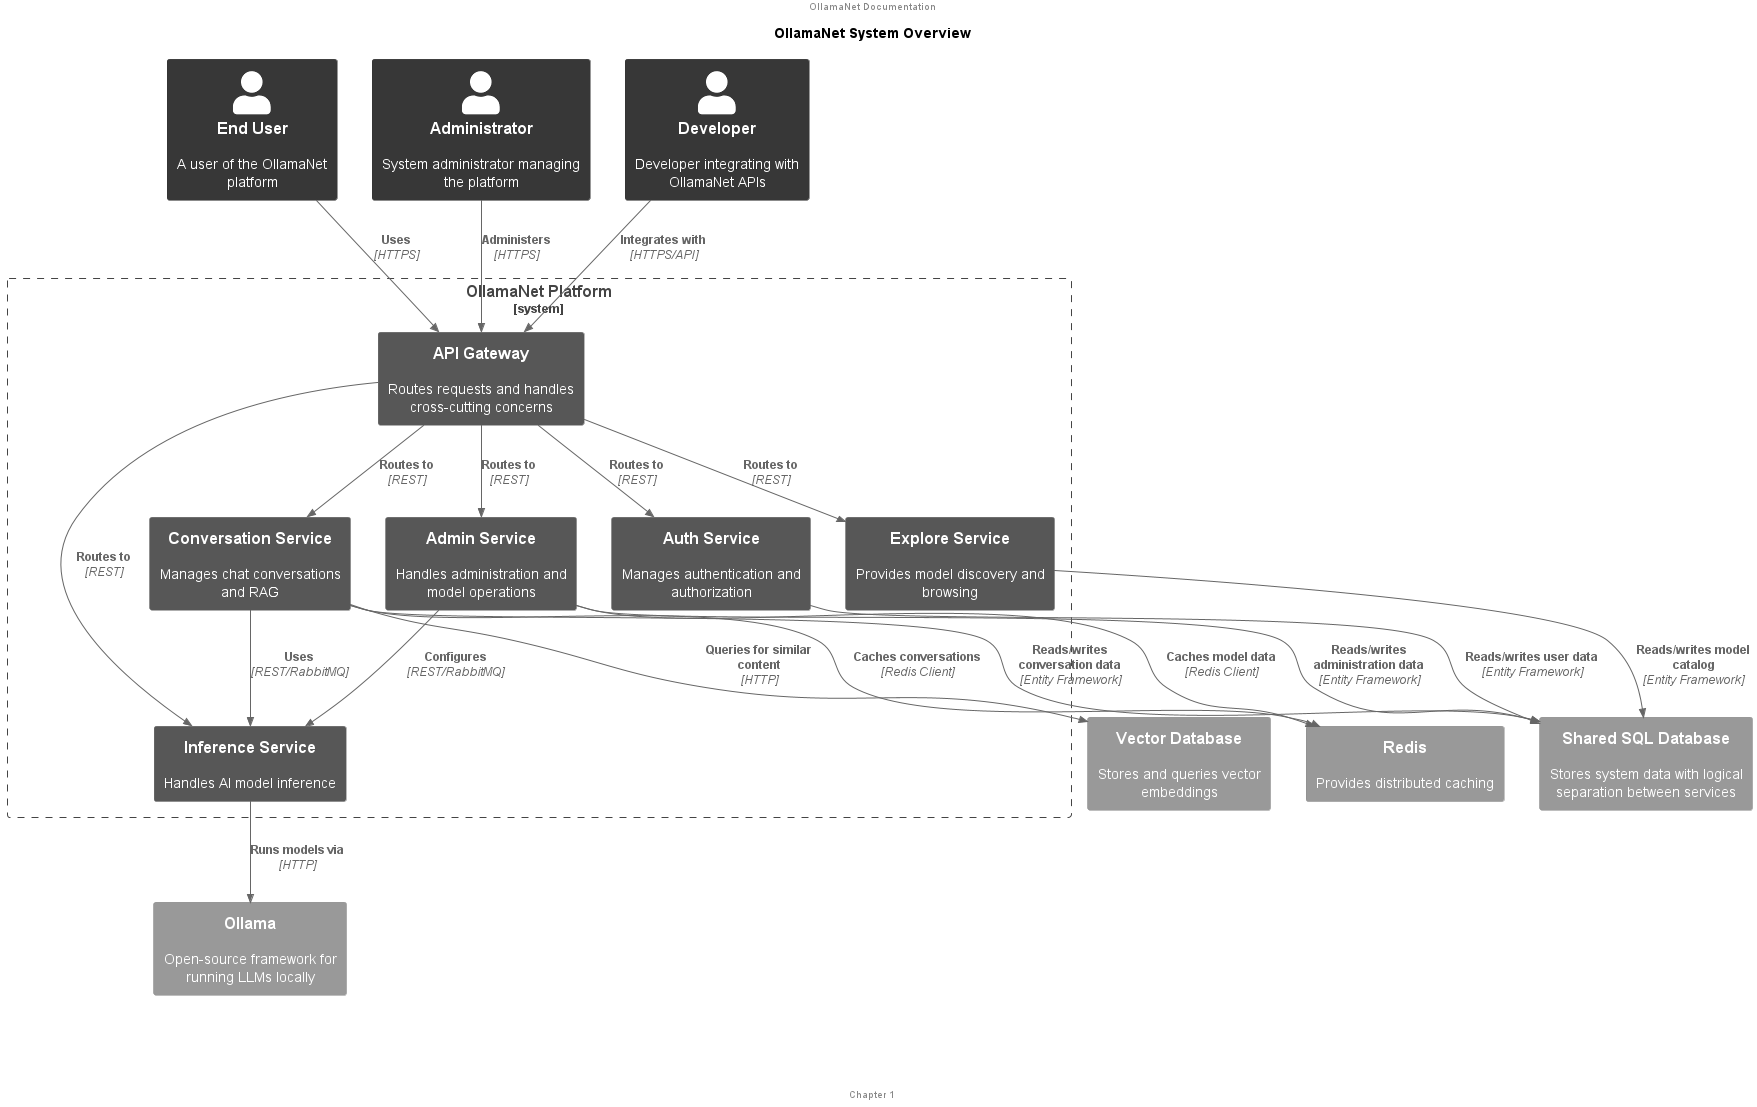
\includegraphics[width=0.8\textwidth]{./Chapter01/figures/OllamaNet_System_Overview.png}
    \caption{OllamaNet Architecture Overview}
    \label{fig:ollamanet-architecture}
\end{figure}

\begin{terminology}
\begin{description}
    \item[OllamaNet:] Comprehensive AI platform with microservices architecture for LLM interaction
    \item[Microservice:] Independent, specialized service with specific domain responsibilities
    \item[LLM:] Large Language Model, an AI model used for text generation and understanding
\end{description}
\end{terminology}

\section{Problem Statement}

Traditional AI model deployment and interaction platforms often face several key challenges:

\begin{enumerate}
    \item \textbf{Complexity in Administration}: Managing AI models, users, and permissions typically requires complex administrative interfaces.
    \item \textbf{Context Loss in Conversations}: Users often lose conversation history and context when interacting with AI models.
    \item \textbf{Inefficient Discovery}: Finding the right AI model for specific needs can be difficult without proper categorization and search capabilities.
    \item \textbf{Security Concerns}: Maintaining proper authentication and authorization across AI services presents security challenges.
    \item \textbf{Performance Bottlenecks}: AI interactions can suffer from latency issues, especially without proper caching and optimization strategies.
    \item \textbf{Data Management Complexity}: Handling the persistence of conversations, user data, and model information requires sophisticated data access patterns.
    \item \textbf{Reliability Constraints}: Many existing solutions use non-relational databases for speed of development, sacrificing data reliability and relationship integrity in the process.
    \item \textbf{Limited Customization}: Popular Python-based LLM libraries prioritize simplicity over extensibility, limiting developers' ability to customize the infrastructure.
\end{enumerate}

OllamaNet addresses these challenges through its specialized microservice architecture, providing a robust, extensible, and maintainable solution for AI model interaction.

\begin{terminology}
\begin{description}
    \item[API Gateway:] Component that routes requests to appropriate microservices
    \item[Context Preservation:] Maintaining conversation history and state across interactions
    \item[Caching:] Storing frequently accessed data to improve performance
\end{description}
\end{terminology}

\section{Objectives and Goals}

The OllamaNet platform aims to achieve the following objectives:

\begin{enumerate}
    \item \textbf{Provide Comprehensive Administration}: Deliver complete control over platform resources through the AdminService.
    \item \textbf{Enable Secure Authentication}: Implement robust user authentication and authorization via the AuthService.
    \item \textbf{Facilitate Model Discovery}: Allow users to browse and evaluate AI models through the ExploreService.
    \item \textbf{Support Rich Conversations}: Enable persistent, organized conversations with AI models via the ConversationService.
    \item \textbf{Ensure Data Integrity}: Maintain consistent data operations through the DB Layer.
    \item \textbf{Optimize Performance}: Implement caching strategies and efficient data access patterns across services.
    \item \textbf{Enhance User Experience}: Deliver a responsive, intuitive interface for all platform interactions.
    \item \textbf{Enable Custom Inference}: Provide flexible AI model inference capabilities through the InferenceService.
\end{enumerate}

These objectives are achieved through a carefully designed microservices architecture that emphasizes separation of concerns, domain-driven design, and robust integration patterns.

\begin{terminology}
\begin{description}
    \item[Domain-Driven Design:] Software development approach that focuses on the core domain and domain logic
    \item[Separation of Concerns:] Design principle for separating software into distinct sections
    \item[Integration Pattern:] Standardized approach for connecting different components or services
\end{description}
\end{terminology}

\section{Project Scope}

OllamaNet encompasses a full-stack solution with the following components:

\subsection{Microservices Backend}
\begin{itemize}
    \item \textbf{AdminService}: Central control point for platform administration, managing users, AI models, tags, and inference operations.
    \item \textbf{AuthService}: Comprehensive authentication and authorization service handling user registration, login, password management, and role-based access control.
    \item \textbf{ExploreService}: Model discovery and browsing service allowing users to search, filter, and explore available AI models and their capabilities.
    \item \textbf{ConversationService}: Conversation management service enabling persistent, organized interactions with AI models, including real-time streaming responses.
    \item \textbf{InferenceService}: Flexible inference engine service for interacting with Ollama models, exposed via ngrok for accessibility.
    \item \textbf{Gateway}: API gateway service routing client requests to appropriate microservices, handling authentication and authorization.
    \item \textbf{DB Layer}: Shared data access infrastructure implementing the repository and unit of work patterns for consistent data operations.
\end{itemize}

\subsection{Frontend Applications}
\begin{itemize}
    \item Administrative interfaces for platform management
    \item End-user interfaces for conversation and model exploration
\end{itemize}

\subsection{Infrastructure Components}
\begin{itemize}
    \item SQL Server database for persistence
    \item Redis for distributed caching
    \item JWT-based authentication system
    \item Integration with the Ollama inference engine
    \item RabbitMQ for service discovery
\end{itemize}

\begin{figure}
    \centering
    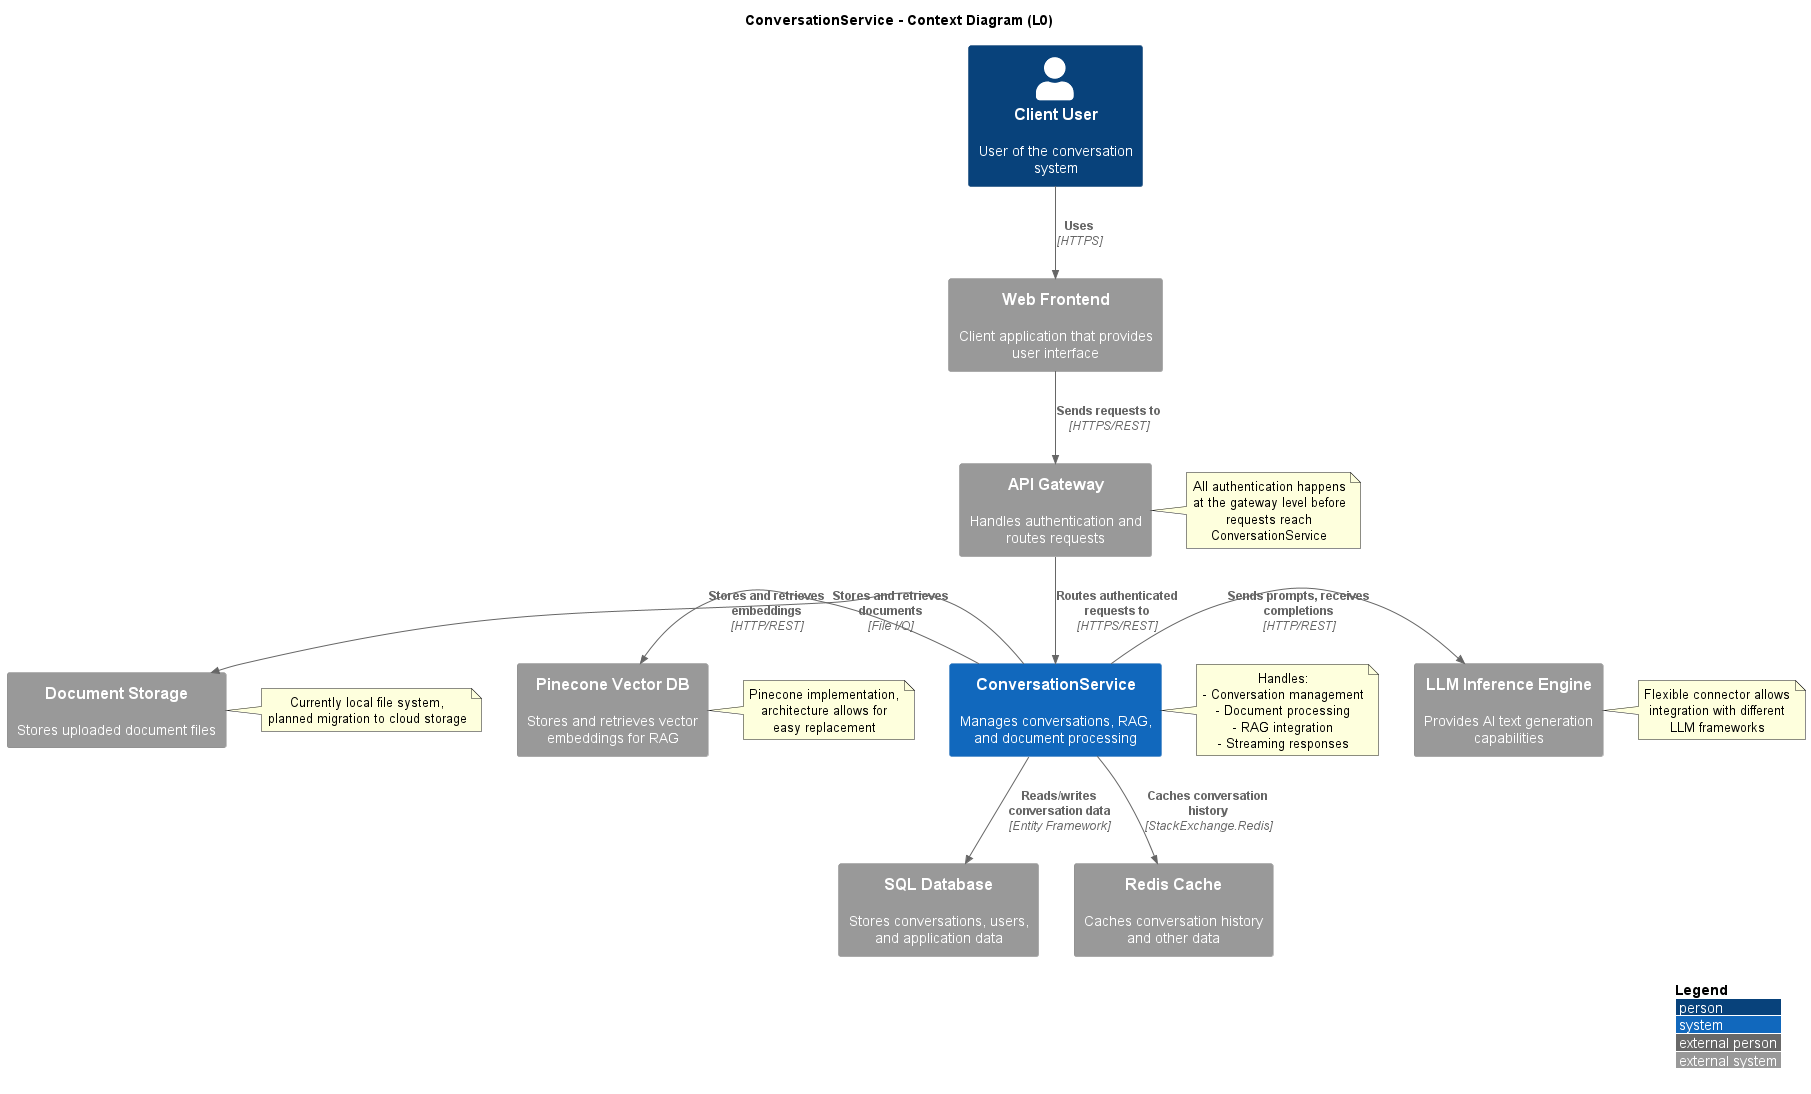
\includegraphics[width=0.8\textwidth]{./Chapter01/figures/ConversationService_Context.png}
    \caption{OllamaNet Platform Components}
    \label{fig:ollamanet-platform-components}
\end{figure}

\begin{terminology}
\begin{description}
    \item[Repository Pattern:] Design pattern that mediates between the domain and data mapping layers
    \item[Unit of Work:] Pattern that maintains a list of objects affected by a business transaction
    \item[JWT:] JSON Web Token, a secure method for representing claims between parties
    \item[Redis:] In-memory data structure store used for caching
    \item[RabbitMQ:] Message broker software for service-to-service communication
\end{description}
\end{terminology}

\section{Implementation Strategy}

OllamaNet follows a structured implementation approach:

\begin{enumerate}
    \item \textbf{Service Isolation}: Each microservice addresses a specific domain with clear boundaries, following domain-driven design principles.
    \item \textbf{Shared Data Layer}: A common DB layer provides consistent data access patterns across all services.
    \item \textbf{API-First Design}: RESTful APIs with comprehensive documentation via Swagger/OpenAPI ensure clear service interfaces.
    \item \textbf{Progressive Enhancement}: Services evolve through phased migrations and improvements, with clear versioning.
    \item \textbf{Performance Optimization}: Strategic caching and efficient data access patterns ensure responsive user experiences.
    \item \textbf{Security Integration}: Consistent authentication and authorization across services protect resources.
    \item \textbf{Domain-Driven Design}: Service organization based on business domains and use cases ensures alignment with business needs.
    \item \textbf{Notebook-First Inference}: The InferenceService uses a notebook-based architecture for flexibility and accessibility.
\end{enumerate}

This implementation strategy enables the platform to be both robust and flexible, catering to enterprise-grade requirements while maintaining developer accessibility and extensibility.

\begin{terminology}
\begin{description}
    \item[REST:] Representational State Transfer, an architectural style for designing networked applications
    \item[Swagger/OpenAPI:] Framework for API documentation and specification
    \item[Notebook-First Architecture:] Implementation approach that prioritizes interactive development environments
\end{description}
\end{terminology}

\section{Report Structure}

This documentation is organized to provide a comprehensive understanding of the OllamaNet platform:

\begin{itemize}
    \item \textbf{Chapter 2}: Explores the background and theoretical foundations of microservices architecture
    \item \textbf{Chapter 3}: Details the requirements analysis and domain modeling
    \item \textbf{Chapter 4}: Describes the overall system architecture and communication patterns
    \item \textbf{Chapter 5}: Examines the database layer and data management strategies
    \item \textbf{Chapter 6}: Provides detailed designs for each microservice
    \item \textbf{Chapter 7}: Outlines the frontend architecture and integration
    \item \textbf{Chapter 8}: Explains the testing strategy across services
    \item \textbf{Chapter 9}: Covers implementation details and development practices
    \item \textbf{Chapter 10}: Presents system evaluation and performance metrics
    \item \textbf{Chapter 11}: Concludes with lessons learned and future directions
\end{itemize}

Each chapter builds on the previous to create a complete picture of the OllamaNet platform's architecture, implementation, and value proposition.

\begin{terminology}
\begin{description}
    \item[Architecture:] The high-level structure of a software system
    \item[Domain Model:] Conceptual model of the domain that incorporates both behavior and data
    \item[Communication Pattern:] Standard approach for service interactions in a distributed system
\end{description}
\end{terminology}






\cleardoublepage
\def\chapdir{./Chapter02}

\chapter{Background \& Literature Review} \label{ch:background}

\section{Theoretical Background}

The OllamaNet platform is built on several key theoretical foundations that inform its architecture and design:

\subsection{Microservices Architecture}

Microservices architecture represents a modern approach to software development where applications are composed of small, independent services that communicate over well-defined APIs. This architectural style has gained prominence as an alternative to monolithic applications, offering benefits such as:

\begin{itemize}
    \item \textbf{Independent Deployability}: Each service can be deployed, upgraded, and scaled independently
    \item \textbf{Technology Diversity}: Different services can use different technologies based on their specific requirements
    \item \textbf{Focused Development Teams}: Teams can focus on specific business domains and services
    \item \textbf{Resilience}: Failures in one service can be isolated without affecting the entire system
    \item \textbf{Scalability}: Services can be individually scaled based on demand
\end{itemize}

For OllamaNet, microservices architecture enables the separation of concerns between different aspects of the platform (authentication, administration, conversations, exploration, inference) while allowing for independent evolution of each component.

\begin{figure}
    \centering
    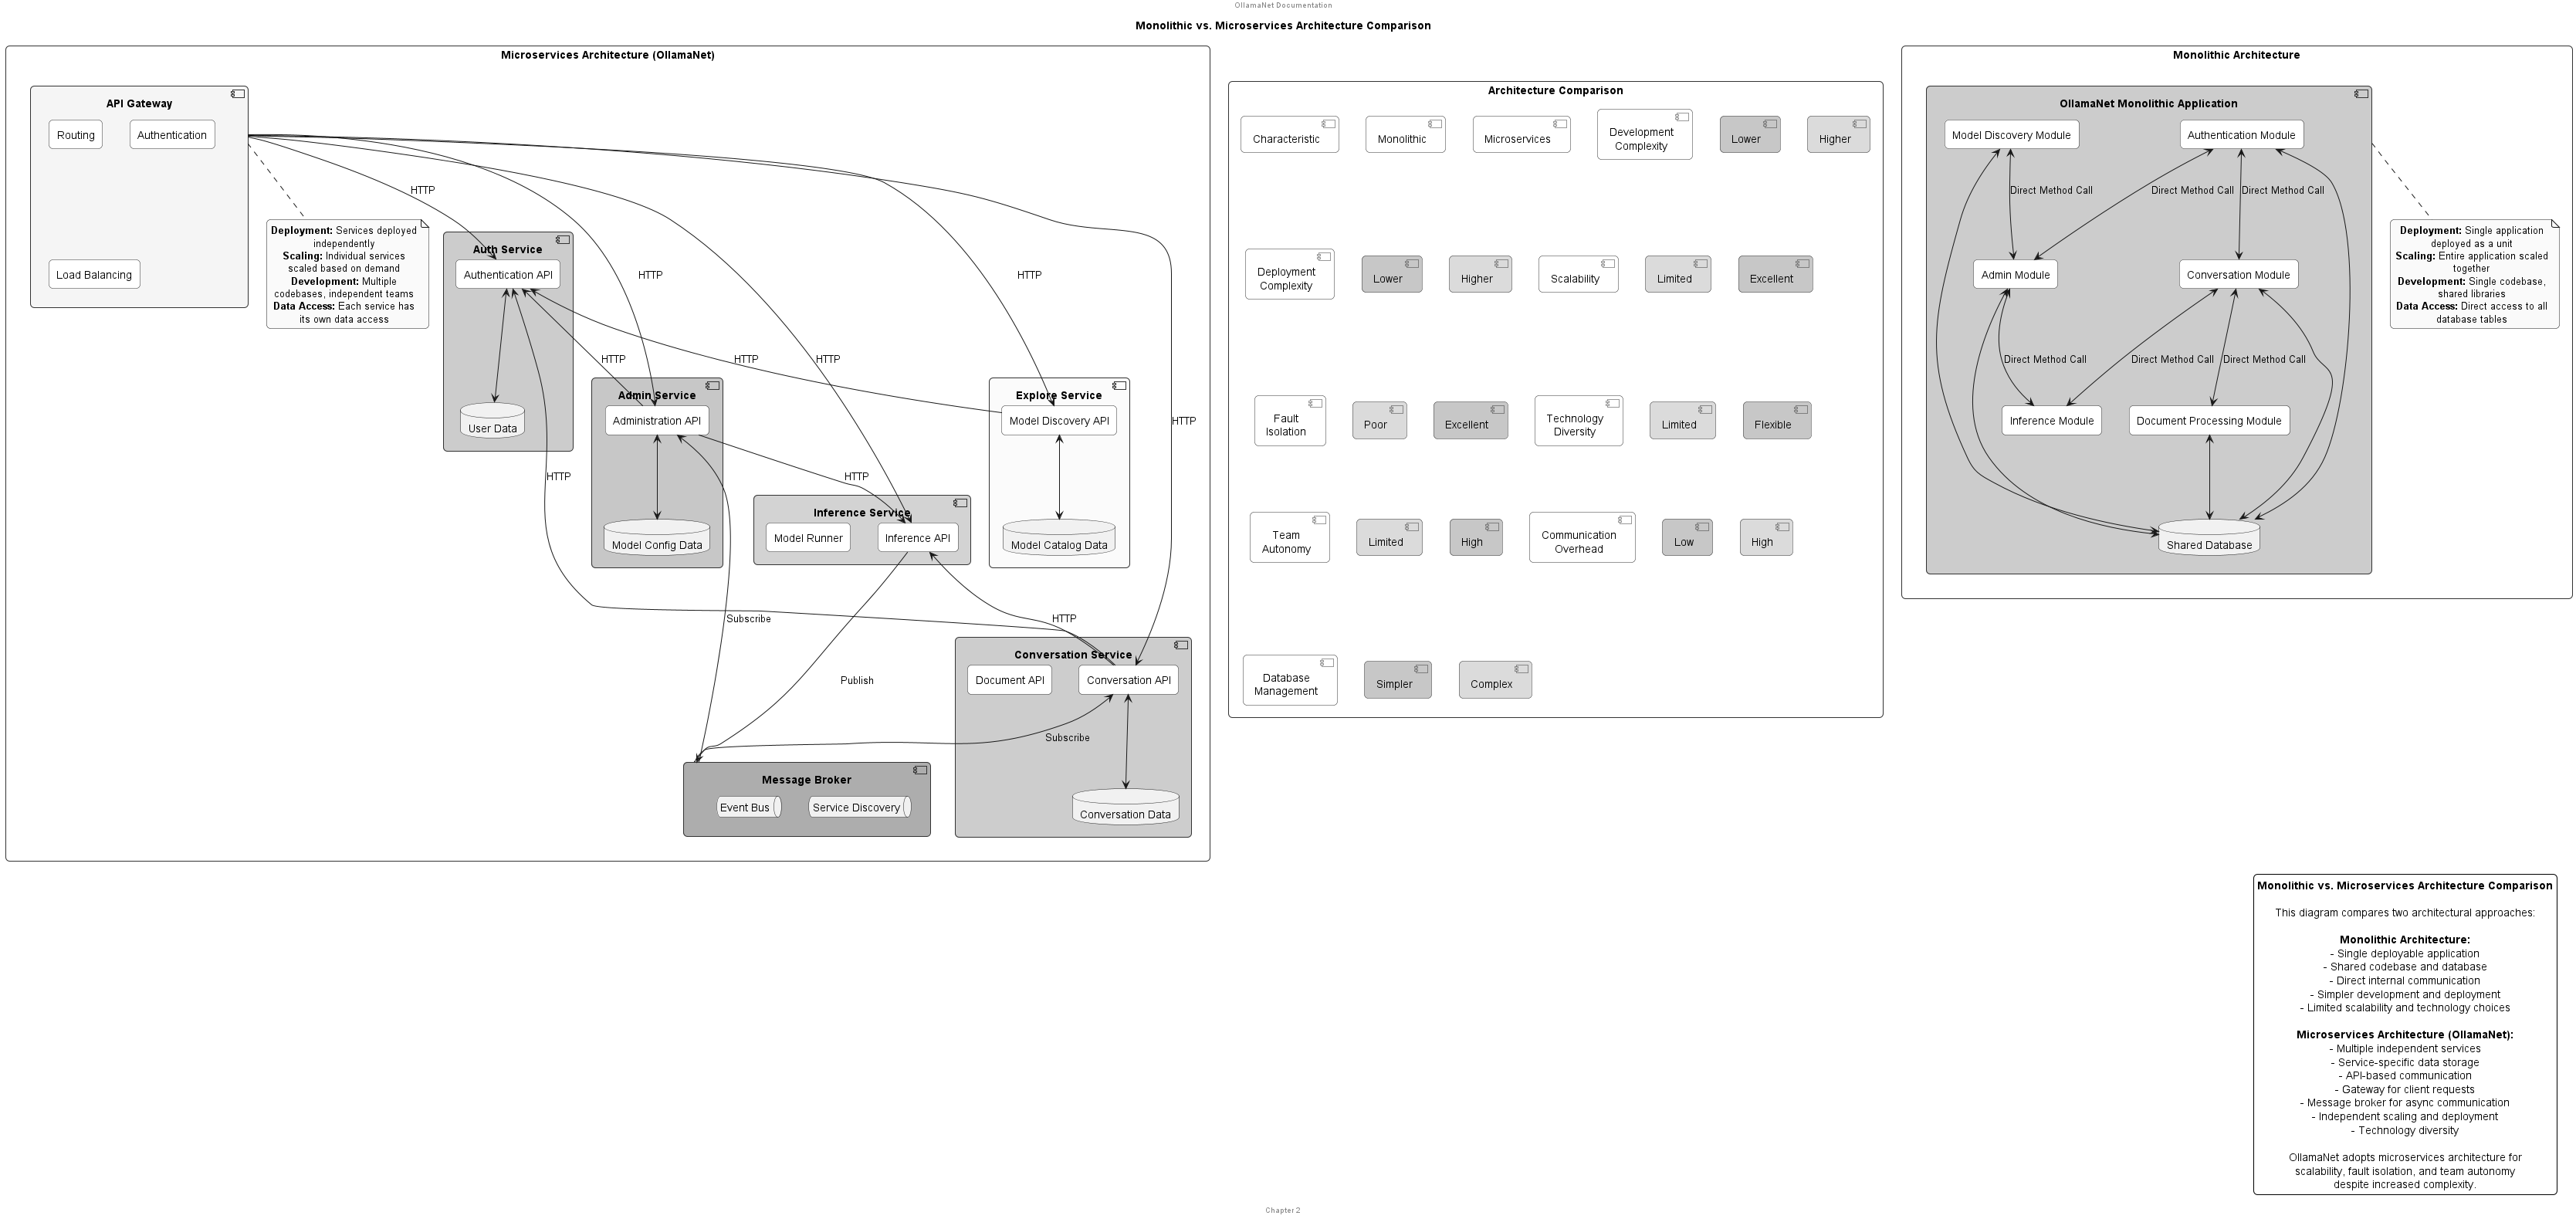
\includegraphics[width=0.9\textwidth]{./Chapter02/figures/Monolithic_vs_Microservices.png}
    \caption{Monolithic vs Microservices Architecture}
    \label{fig:mono-vs-micro}
\end{figure}

\begin{terminology}
\begin{description}
    \item[Microservice:] An architectural style that structures an application as a collection of services that are independently deployable
    \item[API Gateway:] A server that acts as an API front-end, receiving API requests and routing them to appropriate services
\end{description}
\end{terminology}

\subsection{Domain-Driven Design}

Domain-Driven Design (DDD) is a software development approach that focuses on modeling the software to match the business domain. It involves:

\begin{itemize}
    \item \textbf{Ubiquitous Language}: A common language shared between developers and domain experts
    \item \textbf{Bounded Contexts}: Explicit boundaries between different domain models
    \item \textbf{Entities and Value Objects}: Clear modeling of domain objects based on identity and characteristics
    \item \textbf{Aggregates}: Clusters of domain objects treated as a unit for data changes
    \item \textbf{Domain Services}: Operations that don't naturally belong to any specific entity
\end{itemize}

OllamaNet employs DDD principles to ensure each microservice accurately represents its domain model (administration, authentication, conversations, exploration, inference) with appropriate boundaries and clear separation of concerns. This approach resulted in well-defined service boundaries that align with business capabilities.

\begin{figure}
    \centering
    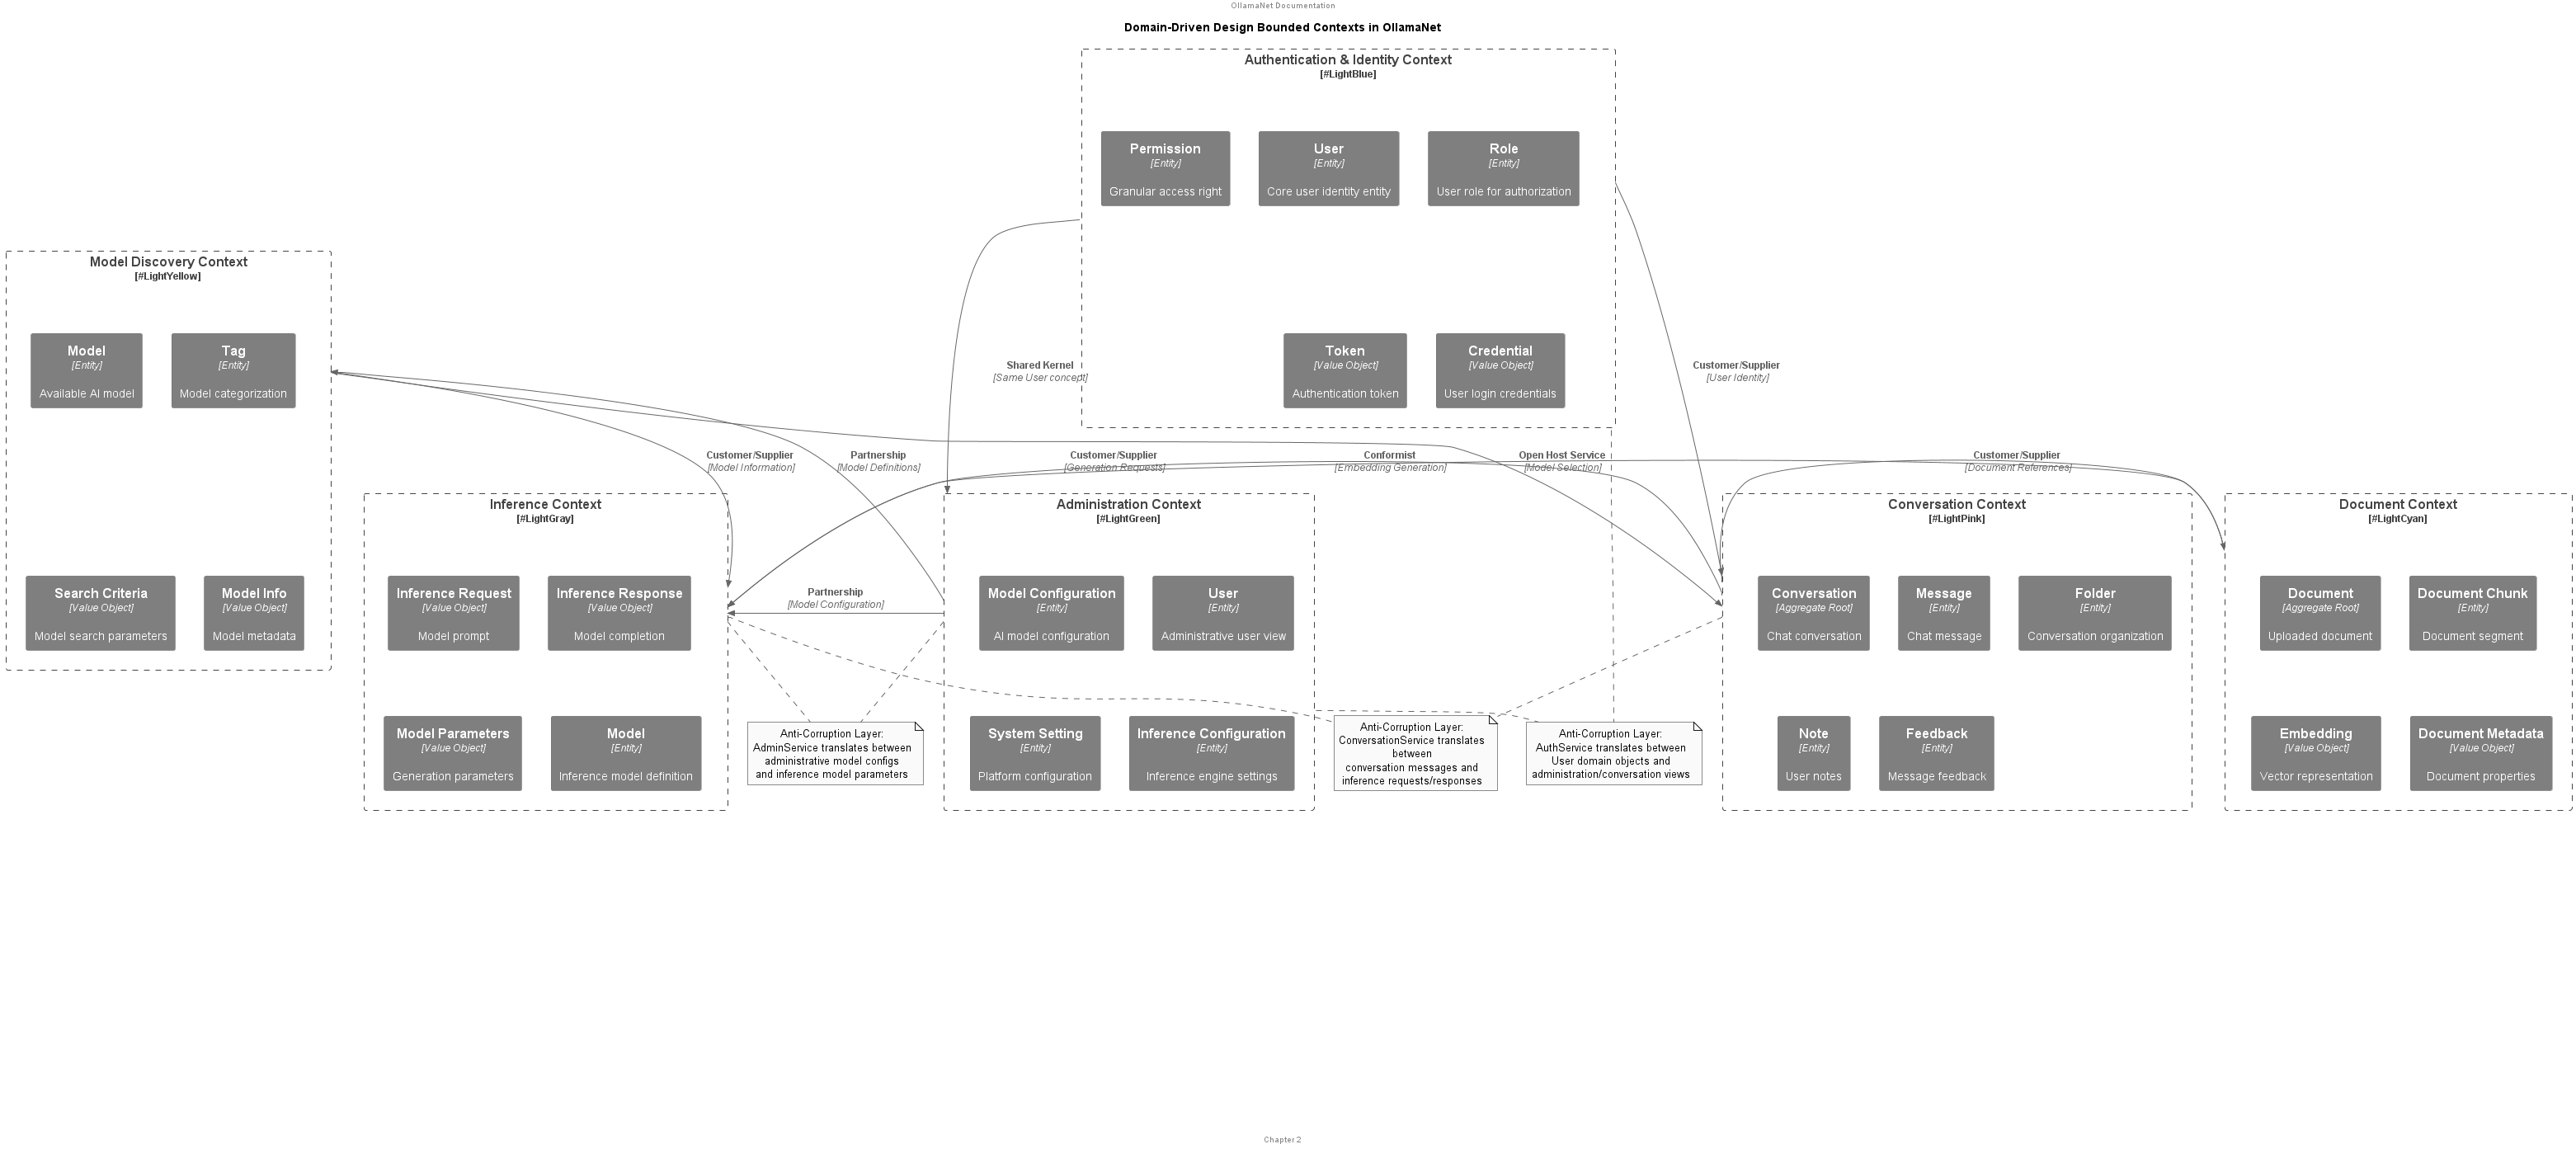
\includegraphics[width=0.9\textwidth]{./Chapter02/figures/DDD_Bounded_Contexts.png}
    \caption{Domain-Driven Design Bounded Contexts}
    \label{fig:ddd-contexts}
\end{figure}

\begin{terminology}
\begin{description}
    \item[Bounded Context:] A conceptual boundary within which a particular domain model applies
    \item[Aggregate:] A cluster of domain objects that can be treated as a single unit
    \item[Ubiquitous Language:] A common language used by developers and domain experts to describe domain concepts
\end{description}
\end{terminology}

\subsection{API Design and RESTful Principles}

The OllamaNet platform follows RESTful API design principles across all its services:

\begin{itemize}
    \item \textbf{Resource-Oriented}: APIs are designed around resources (conversations, models, users)
    \item \textbf{Standard HTTP Verbs}: GET, POST, PUT, DELETE are used for CRUD operations
    \item \textbf{Stateless Communication}: Each request contains all necessary information
    \item \textbf{Standardized Response Formats}: Consistent JSON responses with appropriate HTTP status codes
    \item \textbf{Versioning}: API versioning to support evolution without breaking changes
    \item \textbf{Clear Endpoint Naming}: Intuitive and descriptive endpoint paths
\end{itemize}

These principles ensure consistency across services and ease of integration for client applications.

\subsection{Authentication and Authorization Theories}

OllamaNet implements a robust authentication and authorization system using established security patterns:

\begin{itemize}
    \item \textbf{Token-Based Authentication}: Using JWT (JSON Web Tokens) for secure, stateless authentication
    \item \textbf{Claims-Based Identity}: User information stored as claims within tokens
    \item \textbf{Role-Based Access Control}: Permissions assigned based on user roles
    \item \textbf{Refresh Token Pattern}: Long-lived refresh tokens used to obtain new access tokens
    \item \textbf{Token Validation}: Comprehensive validation of token signature, expiry, and claims
    \item \textbf{Gateway Authentication}: Centralized authentication at the API Gateway level
\end{itemize}

\subsection{Caching Strategies and Patterns}

The platform implements several caching strategies to optimize performance:

\begin{itemize}
    \item \textbf{Distributed Caching}: Redis used as a shared cache across services
    \item \textbf{Cache-Aside Pattern}: Data retrieved from cache first, falling back to the database
    \item \textbf{Expiration Policies}: Time-based expiration tailored to data volatility
    \item \textbf{Cache Invalidation}: Strategies to update or invalidate cached data when modified
    \item \textbf{Multi-Level Caching}: In-memory and distributed caching used in tandem
    \item \textbf{Resilient Caching}: Graceful fallback when cache is unavailable
\end{itemize}

\subsection{Distributed Systems Concepts}

As a distributed system, OllamaNet addresses several core distributed computing challenges:

\begin{itemize}
    \item \textbf{Service Discovery}: Using message brokers (RabbitMQ) for dynamic service URL updates
    \item \textbf{Consistency Models}: Ensuring data consistency across services
    \item \textbf{Failure Handling}: Strategies for graceful degradation when components fail
    \item \textbf{Distributed Tracing}: Request tracing across service boundaries
    \item \textbf{Eventual Consistency}: Accepting temporary inconsistency for system availability
    \item \textbf{Circuit Breaking}: Preventing cascading failures across service calls
\end{itemize}

\begin{terminology}
\begin{description}
    \item[REST:] Representational State Transfer, an architectural style for distributed hypermedia systems
    \item[JWT:] JSON Web Token, a compact, URL-safe means of representing claims to be transferred between two parties
    \item[Caching:] Storing copies of data in a high-speed data store to reduce database load
\end{description}
\end{terminology}

\section{Similar Systems Analysis}

Several existing AI platforms offer similar functionality to OllamaNet, though often with different architectural approaches:

\subsection*{OpenAI API Platform}
\begin{itemize}
    \item \textbf{Architecture}: Centralized API services with limited customization
    \item \textbf{Strengths}: Enterprise-grade security, high-reliability, extensive model selection
    \item \textbf{Limitations}: Limited local deployment options, proprietary technology stack, higher cost
    \item \textbf{Comparison}: OllamaNet provides greater customization, local deployment, and cost advantages
\end{itemize}

\subsection*{Hugging Face Spaces}
\begin{itemize}
    \item \textbf{Architecture}: Model hosting platform with standardized deployment
    \item \textbf{Strengths}: Wide model availability, community-driven, integrated UI components
    \item \textbf{Limitations}: Less focus on enterprise features, limited conversation persistence
    \item \textbf{Comparison}: OllamaNet offers stronger administrative controls and conversation management
\end{itemize}

\subsection*{LangChain}
\begin{itemize}
    \item \textbf{Architecture}: Python framework for LLM development, not a complete platform
    \item \textbf{Strengths}: Extensive integrations, component-based architecture, rapid prototyping
    \item \textbf{Limitations}: Python-centric, less focus on enterprise deployment, limited built-in UI
    \item \textbf{Comparison}: OllamaNet provides a complete, production-ready system vs. a development framework
\end{itemize}

\subsection*{LocalAI}
\begin{itemize}
    \item \textbf{Architecture}: Local API server for open-source models
    \item \textbf{Strengths}: Self-hosted, privacy-focused, open-source
    \item \textbf{Limitations}: Limited administrative features, Python-based implementation
    \item \textbf{Comparison}: OllamaNet offers more comprehensive microservices with better separation of concerns
\end{itemize}

\subsection*{Ollama (Base System)}
\begin{itemize}
    \item \textbf{Architecture}: Single-service model server
    \item \textbf{Strengths}: Easy setup, rapidly growing ecosystem, excellent command-line interface
    \item \textbf{Limitations}: Limited administrative features, basic conversation management
    \item \textbf{Comparison}: OllamaNet extends Ollama's capabilities with robust microservices around it
\end{itemize}

A key advantage of OllamaNet over these systems is its comprehensive microservices approach with strong domain separation, robust database structure, and enterprise-grade features while maintaining the ability to leverage open-source models.

\section{Technologies Evaluation}

The OllamaNet platform has been built using a carefully selected technology stack:

\subsection*{Backend Framework}

\textbf{ASP.NET Core (.NET 9.0)} was chosen as the primary backend framework for all microservices due to:
\begin{itemize}
    \item Performance advantages and scalability
    \item Comprehensive support for RESTful API development
    \item Strong typing and compile-time safety
    \item Rich ecosystem of libraries and tools
    \item Cross-platform capabilities
    \item Superior robustness compared to popular Python-based LLM libraries
    \item Enhanced customizability and extensibility for enterprise implementations
    \item Better thread management for handling concurrent LLM operations
\end{itemize}

The decision to use C\# and .NET over Python (the most common language for LLM applications) was deliberate, prioritizing long-term maintainability, performance, and enterprise-grade stability over the rapid prototyping advantages of Python libraries. This choice enables developers to build custom extensions and integrations with greater confidence in the system's reliability and scalability.

\subsection*{Database Technologies}

\textbf{SQL Server} serves as the primary database technology, offering:
\begin{itemize}
    \item Strong ACID compliance for transactional integrity
    \item Robust performance for relational data
    \item Comprehensive tooling and management capabilities
    \item Strong integration with Entity Framework Core
    \item Superior data reliability compared to non-relational alternatives
\end{itemize}

OllamaNet deliberately employs a relational database schema rather than trending non-relational approaches. While non-relational databases offer faster development cycles and simpler initial setup, the project prioritizes data reliability, relationship integrity, and consistent query performance. This approach ensures conversations, user data, and model information maintain their referential integrity and can be reliably retrieved with consistent performance characteristics, even as the data grows in complexity and volume.

\textbf{Redis} provides distributed caching capabilities, delivering:
\begin{itemize}
    \item High-performance in-memory data storage
    \item Support for various data structures
    \item Pub/Sub capabilities for real-time features
    \item Distributed caching across services
\end{itemize}

\subsection*{Authentication \& Authorization}

\textbf{JWT (JSON Web Tokens)} with refresh token functionality was implemented for:
\begin{itemize}
    \item Stateless authentication between services
    \item Secure transmission of claims
    \item Support for token expiration and renewal
    \item Cross-service authorization
\end{itemize}

\subsection*{API Documentation}

\textbf{Swagger/OpenAPI} was selected for API documentation because it offers:
\begin{itemize}
    \item Interactive API exploration and testing
    \item Automatic documentation generation
    \item Client code generation capabilities
    \item Standardized API specifications
\end{itemize}

\subsection*{ORM Solution}

\textbf{Entity Framework Core} serves as the object-relational mapping solution, providing:
\begin{itemize}
    \item Clean abstraction over database operations
    \item LINQ support for type-safe queries
    \item Migrations for database schema evolution
    \item Comprehensive relationship mapping
\end{itemize}

\subsection*{Additional Libraries and Tools}
\begin{itemize}
    \item \textbf{FluentValidation}: Comprehensive request validation
    \item \textbf{Polly}: Resilience policies for external service calls
    \item \textbf{OllamaSharp}: Client library for Ollama API integration
    \item \textbf{StackExchange.Redis}: Redis client for distributed caching
    \item \textbf{RabbitMQ Client}: Message broker integration for service discovery
    \item \textbf{Jupyter Notebook} (for InferenceService): Interactive development environment
    \item \textbf{ngrok} (for InferenceService): Secure tunneling for notebook-based services
\end{itemize}

\begin{terminology}
\begin{description}
    \item[ORM:] Object-Relational Mapping, a technique for converting data between incompatible type systems
    \item[ACID:] Atomicity, Consistency, Isolation, Durability - properties of database transactions that guarantee validity
    \item[Pub/Sub:] Publish/Subscribe pattern where senders don't send messages directly to receivers
\end{description}
\end{terminology}

\section{Architectural Patterns}

\subsection{Monolithic vs Microservices Comparison}

OllamaNet chose a microservices architecture over a monolithic approach after careful consideration of trade-offs:

\begin{table}[h]
  \centering
  \caption{Comparison between Monolithic and Microservices Approaches}
  \label{tab:mono-vs-micro}
  \begin{tabular}{|l|p{3.5cm}|p{3.5cm}|p{3.5cm}|}
    \hline
    \textbf{Aspect} & \textbf{Monolithic Approach} & \textbf{Microservices Approach} & \textbf{OllamaNet Decision} \\
    \hline
    Deployment & Simple but all-or-nothing & Complex but granular & Microservices for deployment flexibility \\
    \hline
    Development & Simple coordination but coupled & Independent but requires interfaces & Microservices for team autonomy \\
    \hline
    Scaling & Vertical scaling of entire application & Horizontal scaling of specific services & Microservices for targeted scaling \\
    \hline
    Technology & Single technology stack & Technology diversity & Microservices with consistent .NET stack \\
    \hline
    Resilience & Single point of failure & Isolated failures & Microservices for fault isolation \\
    \hline
    Complexity & Lower initial complexity & Higher distributed complexity & Microservices with careful boundary design \\
    \hline
  \end{tabular}
\end{table}

\begin{figure}
    \centering
    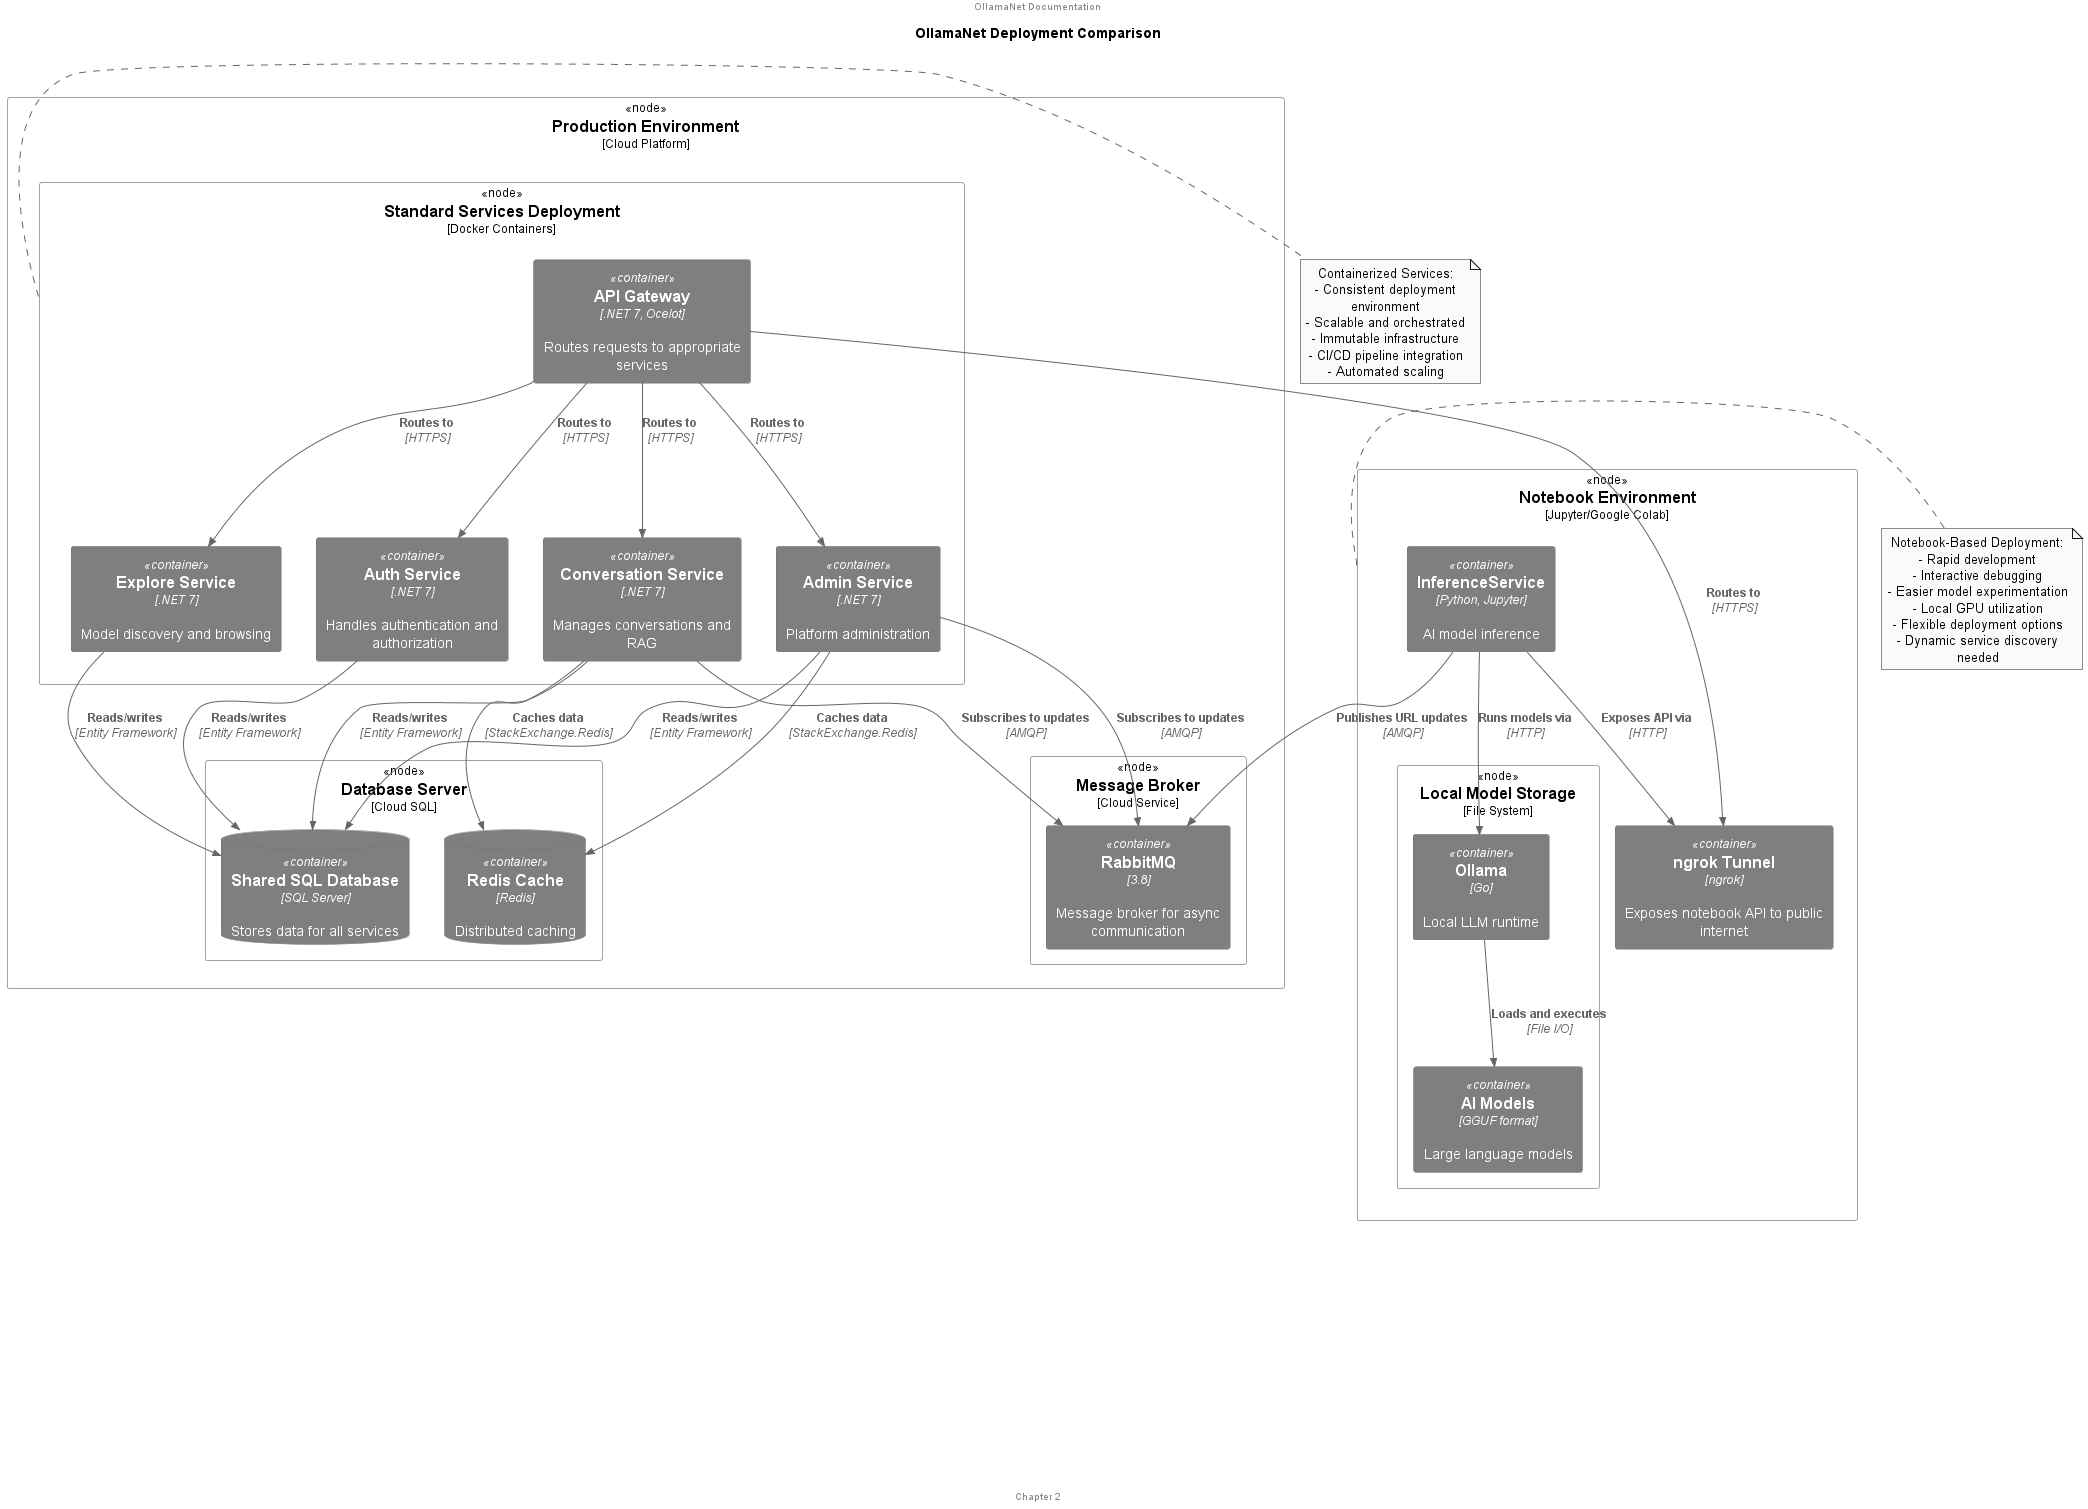
\includegraphics[width=0.8\textwidth]{./Chapter02/figures/Deployment_Comparison.png}
    \caption{Deployment Comparison Between Architectures}
    \label{fig:deploy-comparison}
\end{figure}

\subsection{Microservices Architecture Overview}

OllamaNet implements a microservices architecture with the following characteristics:

\begin{itemize}
    \item \textbf{Service Boundaries}: Services are divided along clear domain boundaries (administration, authentication, conversations, exploration, inference)
    \item \textbf{API Gateway Pattern}: Gateway service provides a single entry point for clients
    \item \textbf{Shared Data Layer}: Common DB layer for consistent data access patterns across services
    \item \textbf{Event-Driven Communication}: Services communicate through events for loose coupling
    \item \textbf{Distributed Caching}: Redis-based caching for performance optimization
    \item \textbf{Authentication Integration}: JWT-based authentication shared across services
    \item \textbf{Service Discovery}: Dynamic discovery of service endpoints, especially critical for the notebook-based InferenceService
\end{itemize}

\begin{figure}
    \centering
    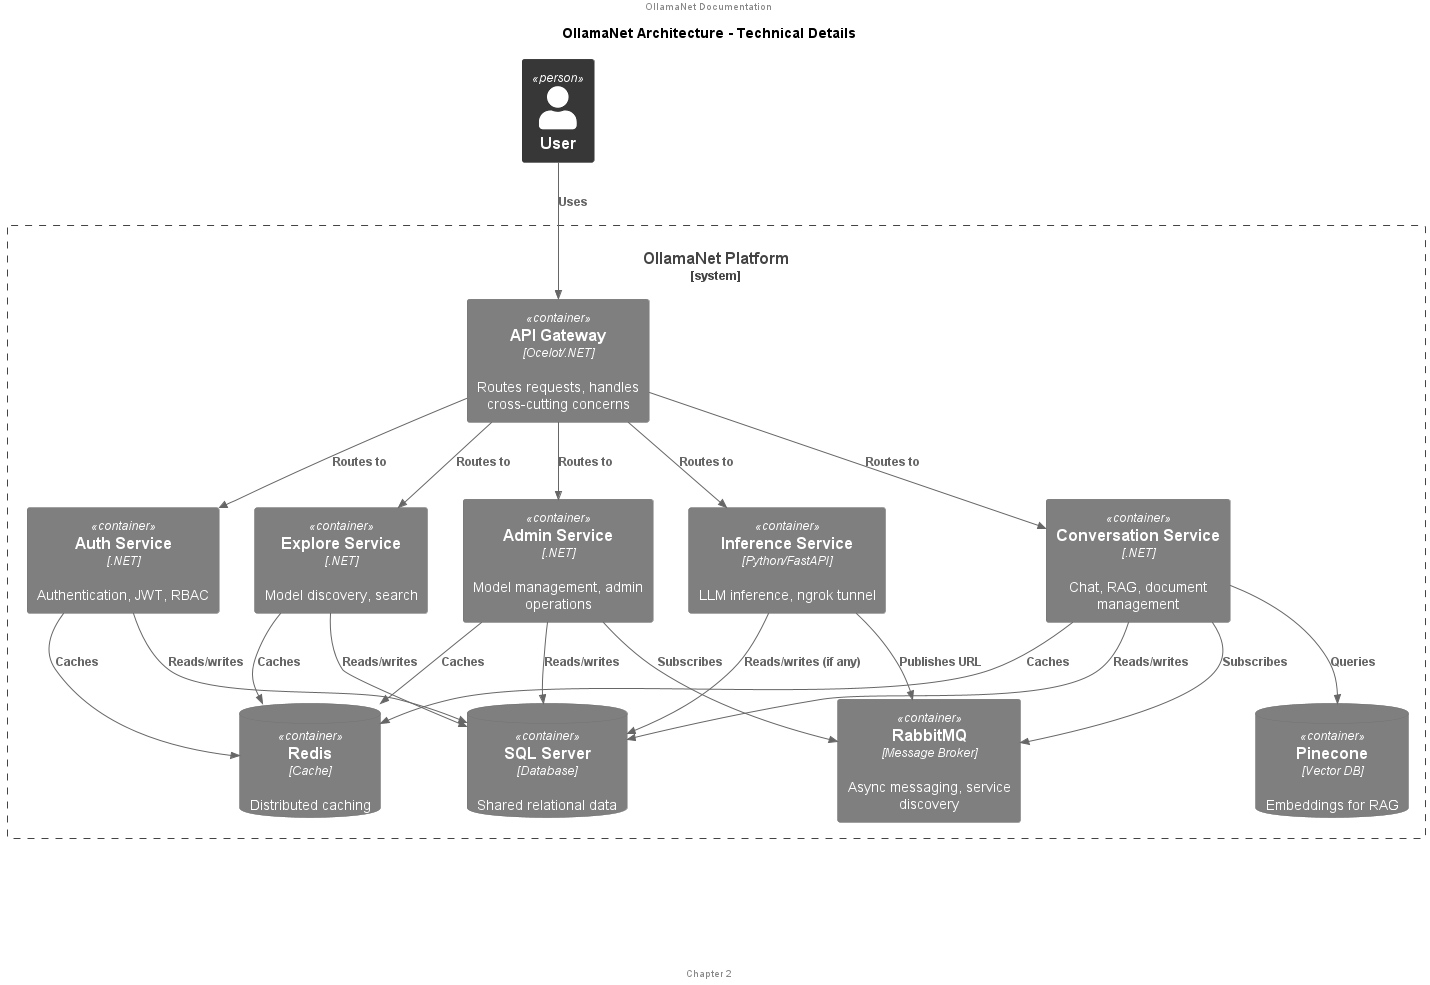
\includegraphics[width=0.9\textwidth]{./Chapter02/figures/OllamaNet_Architecture_Details.png}
    \caption{OllamaNet Microservices Architecture}
    \label{fig:ollamanet-arch-details}
\end{figure}

\subsection{Design Patterns in Microservices}

OllamaNet implements several design patterns to solve common challenges in microservices architecture:

\begin{itemize}
    \item \textbf{Repository Pattern}: Abstracts data access logic from business logic across all services
    \item \textbf{Unit of Work Pattern}: Coordinates operations across multiple repositories
    \item \textbf{Mediator Pattern}: Decouples request handling from business logic
    \item \textbf{Circuit Breaker Pattern}: Prevents cascading failures across services
    \item \textbf{Retry Pattern}: Automatic retry with exponential backoff for transient failures
    \item \textbf{API Gateway Pattern}: Service-specific APIs with consistent patterns
    \item \textbf{Service Discovery Pattern}: Dynamic discovery of service endpoints via RabbitMQ
    \item \textbf{Caching Strategy Pattern}: Multi-level caching for performance optimization
    \item \textbf{Configuration Management Pattern}: Centralized configuration with dynamic updates
    \item \textbf{Decorator Pattern}: Authentication and authorization implemented as decorators
    \item \textbf{Strategy Pattern}: Different services have different routing strategies
\end{itemize}

\begin{figure}
    \centering
    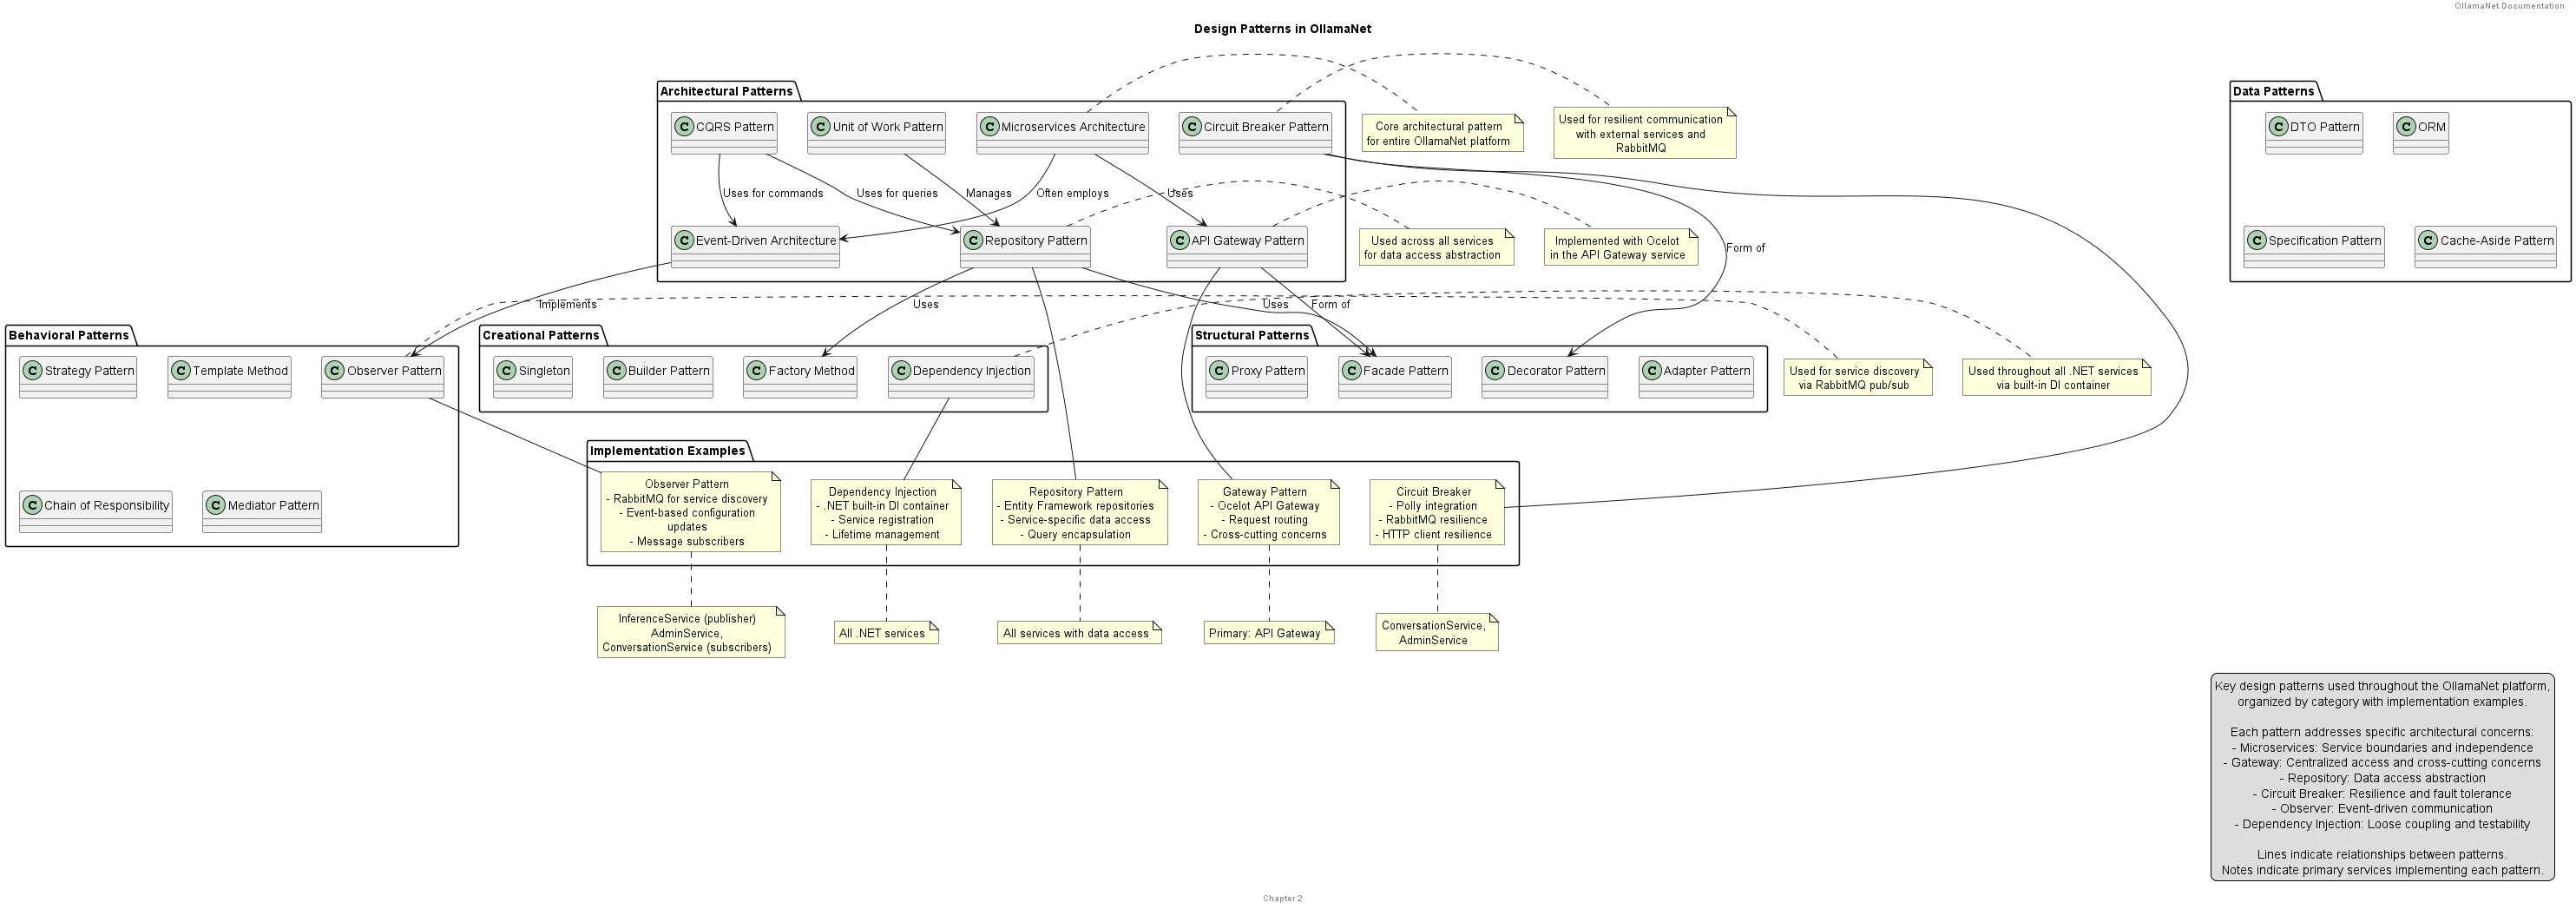
\includegraphics[width=0.8\textwidth]{./Chapter02/figures/Design_Patterns.png}
    \caption{Design Patterns Implementation}
    \label{fig:design-patterns}
\end{figure}

A unique aspect of OllamaNet's design is the notebook-first architecture of the InferenceService, which combines Python flexibility with the robustness of .NET microservices. This service uses ngrok tunneling and RabbitMQ-based service discovery to expose Ollama LLM capabilities from any cloud notebook environment, while maintaining secure integration with the broader platform.

\begin{terminology}
\begin{description}
    \item[Repository Pattern:] A design pattern that mediates between the domain and data mapping layers
    \item[Unit of Work:] A pattern that maintains a list of objects affected by a business transaction
    \item[Circuit Breaker:] A design pattern that detects failures and prevents further requests to failing components
\end{description}
\end{terminology}







\cleardoublepage
\def\chapdir{./Chapter03}

\chapter{Requirements Analysis} \label{ch:requirements}

\section{Stakeholder Analysis}

\subsection{Identification of Key Stakeholders}

The OllamaNet platform serves a diverse group of stakeholders with varying needs and interests:

\begin{enumerate}
   \item \textbf{End Users}
   \begin{itemize}
      \item Regular users seeking AI-powered conversations
      \item Knowledge workers and researchers
      \item Content creators and developers
      \item Students and educators
   \end{itemize}

   \item \textbf{Administrative Personnel}
   \begin{itemize}
      \item Platform administrators
      \item System operators
      \item Security administrators
      \item DevOps engineers
   \end{itemize}

   \item \textbf{Organization Stakeholders}
   \begin{itemize}
      \item IT departments
      \item Management teams
      \item Security and compliance teams
      \item Model development teams
   \end{itemize}

   \item \textbf{Technical Stakeholders}
   \begin{itemize}
      \item Frontend application developers
      \item Integration partners
      \item API consumers
      \item Infrastructure providers
   \end{itemize}

   \item \textbf{Governance Stakeholders}
   \begin{itemize}
      \item Data privacy officers
      \item Compliance managers
      \item Legal representatives
      \item Information security officers
   \end{itemize}
\end{enumerate}

\begin{figure}
    \centering
   %  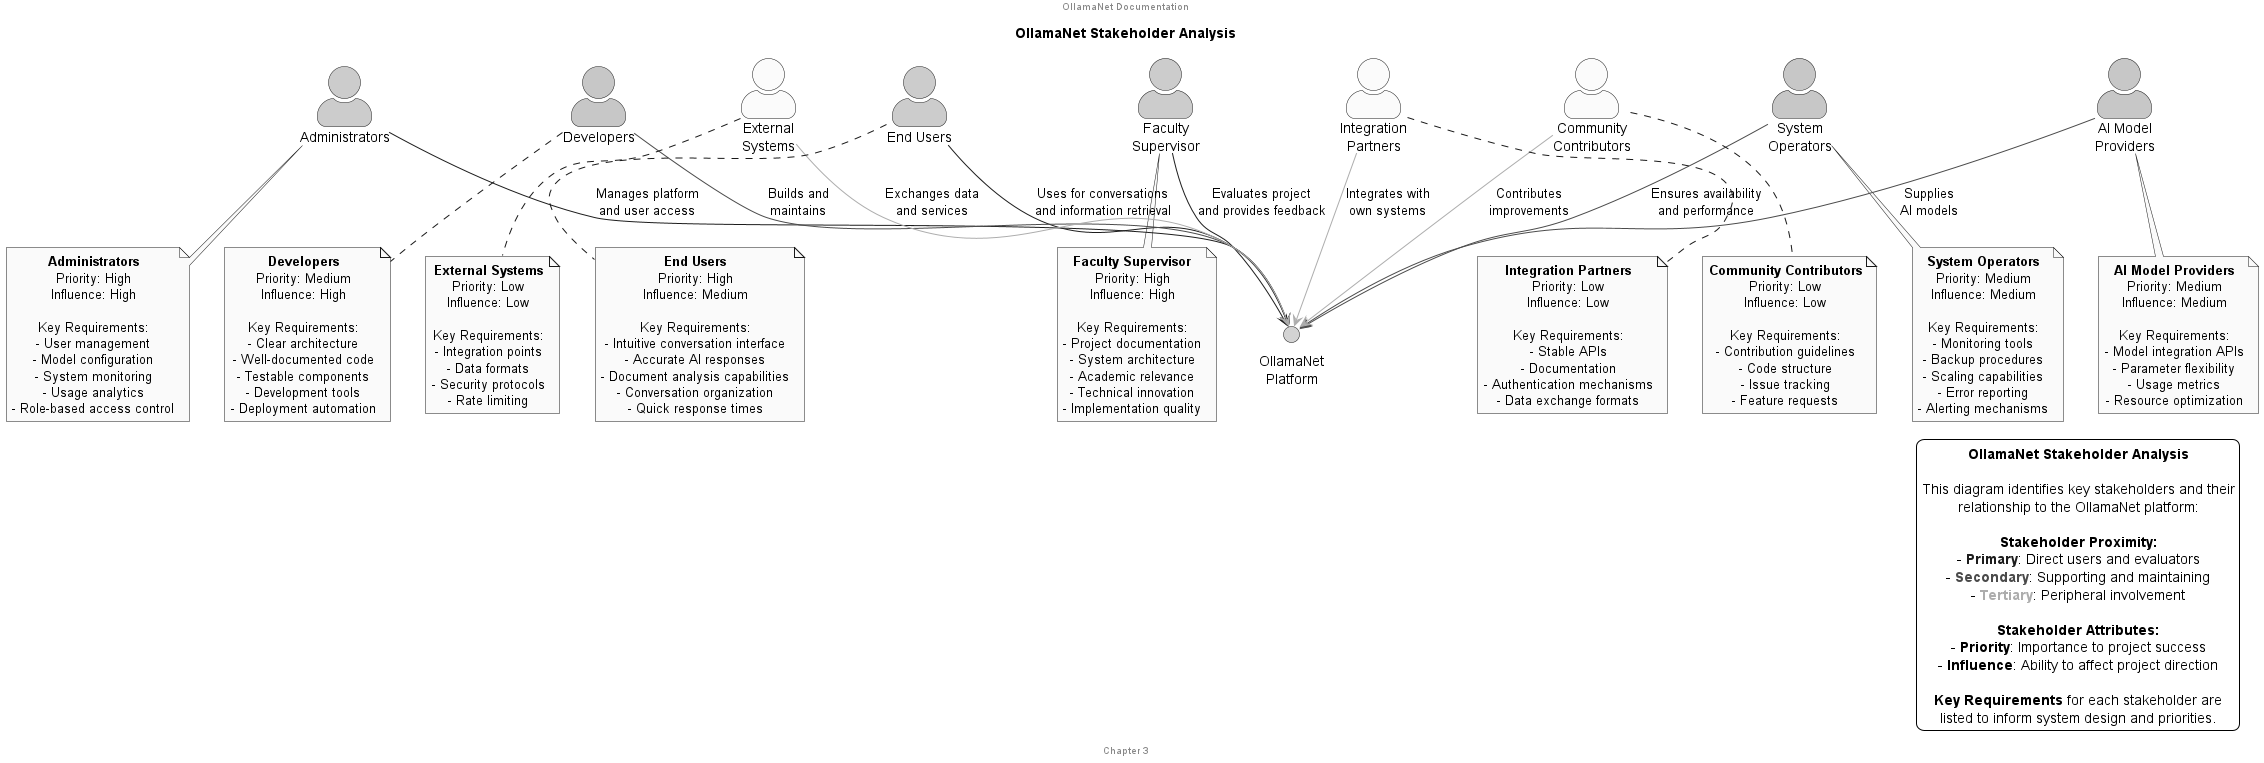
\includegraphics[width=0.8\textwidth]{./Chapter03/figures/Stakeholder_Analysis.png}
    \caption{Stakeholder Analysis Diagram}
    \label{fig:stakeholder-analysis}
\end{figure}

\subsection{Stakeholder Needs and Concerns}

\subsubsection*{End User Needs}
\begin{itemize}
   \item Intuitive and responsive user interface
   \item Persistent conversation history
   \item Well-organized conversation management
   \item Fast and accurate AI responses
   \item Data privacy and security
   \item Seamless authentication
   \item Consistent experience across sessions
   \item Search capabilities for past interactions
   \item Access to a variety of AI models
\end{itemize}

\subsubsection*{Administrative Personnel Needs}
\begin{itemize}
   \item Comprehensive user management capabilities
   \item Fine-grained access control
   \item System monitoring and analytics
   \item Model deployment and management tools
   \item Platform configuration controls
   \item Efficient troubleshooting capabilities
   \item Audit and compliance features
   \item Task automation
\end{itemize}

\subsubsection*{Organization Stakeholders' Concerns}
\begin{itemize}
   \item Total cost of ownership
   \item Compliance with organizational policies
   \item Data security and privacy
   \item User productivity and efficiency
   \item Integration with existing systems
   \item Customization capabilities
   \item Governance and oversight
\end{itemize}

\subsubsection*{Technical Stakeholders' Needs}
\begin{itemize}
   \item Well-documented APIs
   \item Reliable service availability
   \item Consistent data models
   \item Proper error handling
   \item Scalable architecture
   \item Performance optimization
   \item Testability and debugging support
\end{itemize}

\subsubsection*{Governance Stakeholders' Concerns}
\begin{itemize}
   \item Regulatory compliance (GDPR, CCPA, etc.)
   \item Data residency requirements
   \item Audit trails and reporting
   \item Security controls and monitoring
   \item Risk management
   \item Intellectual property protection
\end{itemize}

\subsection{Priority Matrix of Stakeholder Requirements}

The following matrix presents the relative priority of key requirements across different stakeholder groups, rated as High (H), Medium (M), or Low (L) priority:

\begin{table}[h]
  \centering
  \caption{Priority Matrix of Stakeholder Requirements}
  \label{tab:requirement-priority}
  \begin{tabular}{|l|c|c|c|c|c|}
    \hline
    \textbf{Requirement} & \textbf{End Users} & \textbf{Admins} & \textbf{Organization} & \textbf{Technical} & \textbf{Governance} \\
    \hline
    Conversation Persistence & H & L & M & L & M \\
    \hline
    Model Discovery & H & M & M & L & L \\
    \hline
    User Authentication & M & H & H & M & H \\
    \hline
    Admin Controls & L & H & H & L & M \\
    \hline
    Performance & H & M & M & H & L \\
    \hline
    Security & M & H & H & M & H \\
    \hline
    API Access & L & M & L & H & L \\
    \hline
    Data Management & M & H & M & M & H \\
    \hline
    Scalability & L & H & H & H & L \\
    \hline
    Compliance & L & M & H & L & H \\
    \hline
  \end{tabular}
\end{table}

\subsection{Conflicting Requirements and Resolution Approach}

Several areas of potential conflict have been identified between different stakeholders' requirements:

\begin{enumerate}
   \item \textbf{Performance vs. Security}
   \begin{itemize}
      \item \textbf{Conflict}: End users prioritize fast response times, while security stakeholders require thorough validation and protection measures that may introduce latency.
      \item \textbf{Resolution}: Implement performance-optimized security measures, such as caching JWT validation results, using distributed authentication, and implementing parallel processing where possible.
   \end{itemize}

   \item \textbf{Usability vs. Compliance}
   \begin{itemize}
      \item \textbf{Conflict}: Seamless user experience may conflict with compliance requirements for explicit consents and disclosures.
      \item \textbf{Resolution}: Design user-friendly compliance features that integrate organically into the workflow, such as progressive disclosure of terms and just-in-time consent mechanisms.
   \end{itemize}

   \item \textbf{Flexibility vs. Governance}
   \begin{itemize}
      \item \textbf{Conflict}: Technical stakeholders want maximum flexibility and customization, while governance stakeholders require standardization and controlled processes.
      \item \textbf{Resolution}: Implement a modular architecture with clear extension points, coupled with governance policies on which aspects can be customized and how changes are managed.
   \end{itemize}

   \item \textbf{Notebook-First Architecture vs. Reliability}
   \begin{itemize}
      \item \textbf{Conflict}: The InferenceService's notebook-first architecture provides flexibility but creates challenges for reliability and management.
      \item \textbf{Resolution}: Implement robust service discovery mechanisms, monitoring, and auto-recovery while preserving the flexibility of the notebook environment.
   \end{itemize}

   \item \textbf{Centralized vs. Distributed Data}
   \begin{itemize}
      \item \textbf{Conflict}: Performance and user experience benefit from distributed caching, while governance and management prefer centralized control.
      \item \textbf{Resolution}: Implement a hybrid approach with a primary centralized database of record and distributed caching with clear invalidation strategies.
   \end{itemize}
\end{enumerate}

\begin{terminology}
\begin{description}
    \item[Stakeholder:] Any person, group, or organization with an interest in or concern about the project
    \item[Requirements Priority Matrix:] A visualization showing the relative importance of requirements to different stakeholders
\end{description}
\end{terminology}

\section{Functional Requirements}

\subsection{Core Platform Capabilities}

The OllamaNet platform must provide the following core capabilities:

\begin{enumerate}
   \item \textbf{User Authentication and Authorization}
   \begin{itemize}
      \item The system shall provide secure user registration and login facilities
      \item The system shall support role-based access control
      \item The system shall implement JWT-based authentication with refresh token support
      \item The system shall enforce appropriate authorization checks across all services
   \end{itemize}

   \item \textbf{Conversation Management}
   \begin{itemize}
      \item The system shall enable creation, retrieval, update, and deletion of conversations
      \item The system shall maintain conversation history persistently
      \item The system shall support organizing conversations in folders
      \item The system shall provide search functionality for past conversations
      \item The system shall enable real-time streaming of AI responses
   \end{itemize}

   \item \textbf{AI Model Interaction}
   \begin{itemize}
      \item The system shall connect to the Ollama inference engine
      \item The system shall support multiple AI models
      \item The system shall maintain context during conversation
      \item The system shall provide streaming responses for real-time interaction
      \item The system shall support document-based context enhancement
   \end{itemize}

   \item \textbf{Administration and Governance}
   \begin{itemize}
      \item The system shall provide tools for user management
      \item The system shall enable AI model configuration and deployment
      \item The system shall support categorization through a tagging system
      \item The system shall maintain audit logs for administrative actions
      \item The system shall provide monitoring capabilities
   \end{itemize}

   \item \textbf{Content Discovery}
   \begin{itemize}
      \item The system shall enable browsing and searching for AI models
      \item The system shall provide detailed model information
      \item The system shall support filtering models by tags and categories
      \item The system shall optimize discovery through caching
   \end{itemize}
\end{enumerate}

\begin{figure}
    \centering
   %  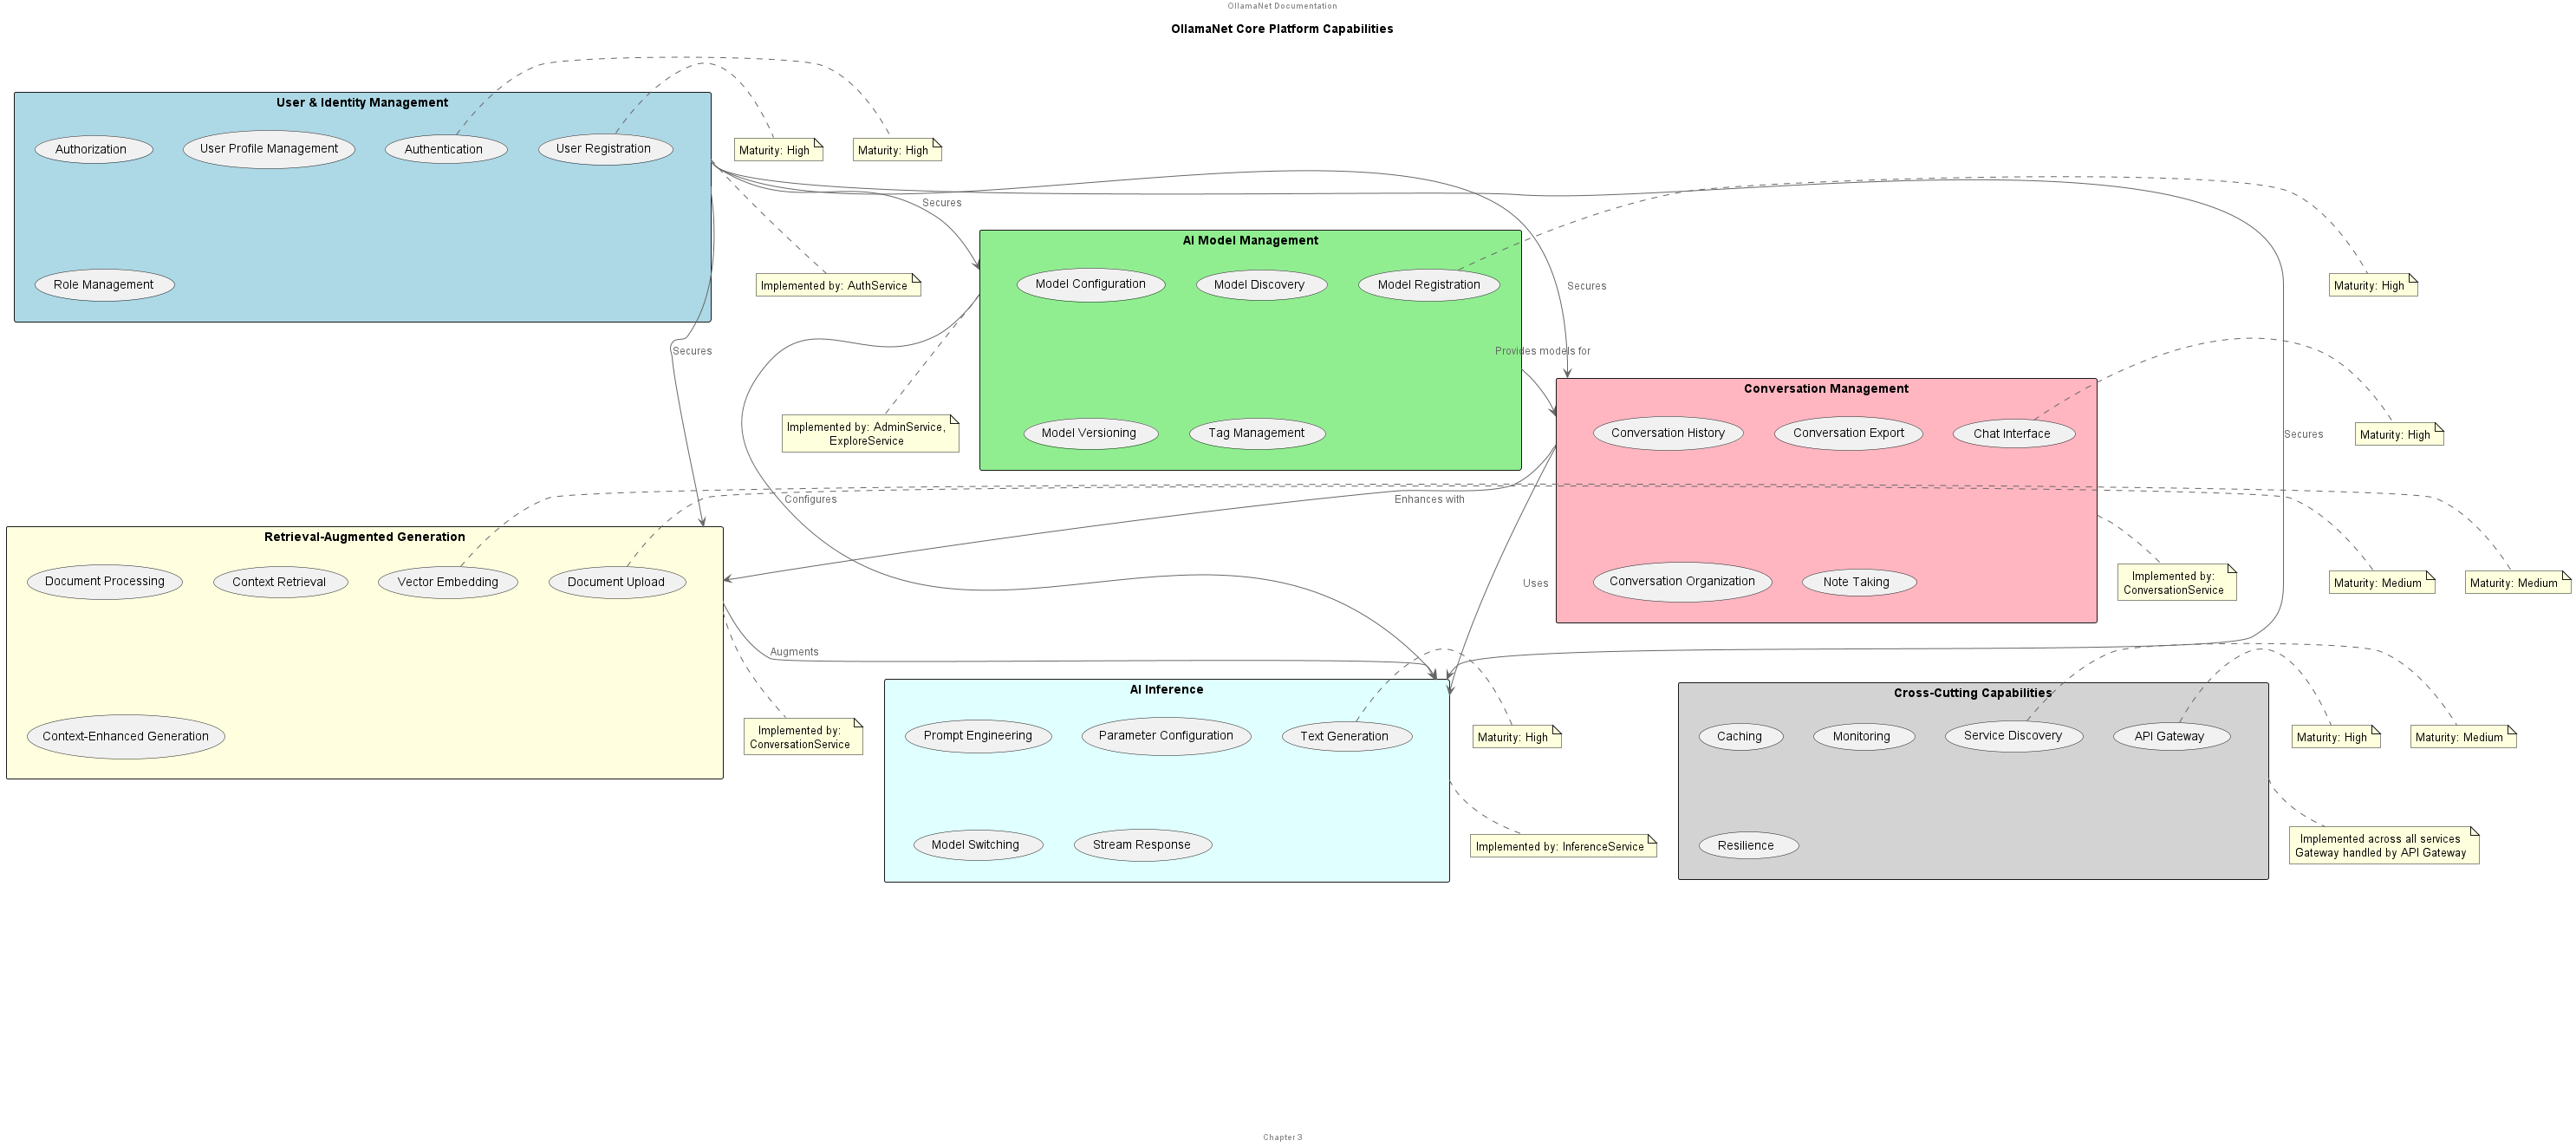
\includegraphics[width=0.8\textwidth]{./Chapter03/figures/Core_Platform_Capabilities.png}
    \caption{Core Platform Capabilities}
    \label{fig:platform-capabilities}
\end{figure}

\subsection{Service-Specific Functionality Requirements}

\subsubsection*{AuthService Requirements}

\begin{enumerate}
   \item \textbf{User Account Management}
   \begin{itemize}
      \item FR-AUTH-01: The service shall allow registration of new users with email, password, and basic profile information
      \item FR-AUTH-02: The service shall validate email addresses through confirmation mechanisms
      \item FR-AUTH-03: The service shall support password reset functionality
      \item FR-AUTH-04: The service shall enforce password complexity requirements
   \end{itemize}

   \item \textbf{Authentication Mechanisms}
   \begin{itemize}
      \item FR-AUTH-05: The service shall authenticate users via username/email and password
      \item FR-AUTH-06: The service shall issue JWT tokens upon successful authentication
      \item FR-AUTH-07: The service shall support refresh tokens for maintaining sessions
      \item FR-AUTH-08: The service shall implement token revocation for security purposes
   \end{itemize}

   \item \textbf{Authorization Management}
   \begin{itemize}
      \item FR-AUTH-09: The service shall support role assignment to users
      \item FR-AUTH-10: The service shall provide APIs for role management
      \item FR-AUTH-11: The service shall enforce role-based access control
      \item FR-AUTH-12: The service shall validate tokens and claims for all protected endpoints
   \end{itemize}
\end{enumerate}

\subsubsection*{AdminService Requirements}

\begin{enumerate}
   \item \textbf{User Administration}
   \begin{itemize}
      \item FR-ADMIN-01: The service shall provide CRUD operations for user management
      \item FR-ADMIN-02: The service shall support role assignment and revocation
      \item FR-ADMIN-03: The service shall enable account status management (activation/deactivation)
      \item FR-ADMIN-04: The service shall support bulk operations for administrative efficiency
   \end{itemize}

   \item \textbf{Model Administration}
   \begin{itemize}
      \item FR-ADMIN-05: The service shall enable registration of AI models with metadata
      \item FR-ADMIN-06: The service shall provide model update and deletion capabilities
      \item FR-ADMIN-07: The service shall support model categorization through tags
      \item FR-ADMIN-08: The service shall allow model activation and deactivation
   \end{itemize}

   \item \textbf{Tag Management}
   \begin{itemize}
      \item FR-ADMIN-09: The service shall provide CRUD operations for tags
      \item FR-ADMIN-10: The service shall enable association of tags with models
      \item FR-ADMIN-11: The service shall support hierarchical tag relationships
      \item FR-ADMIN-12: The service shall provide search and filtering for tags
   \end{itemize}

   \item \textbf{Model Deployment}
   \begin{itemize}
      \item FR-ADMIN-13: The service shall connect to the Ollama API for model operations
      \item FR-ADMIN-14: The service shall support model installation with progress tracking
      \item FR-ADMIN-15: The service shall provide model information retrieval
      \item FR-ADMIN-16: The service shall enable model removal and cleanup
   \end{itemize}
\end{enumerate}

\subsubsection*{ConversationService Requirements}

\begin{enumerate}
   \item \textbf{Conversation Management}
   \begin{itemize}
      \item FR-CONV-01: The service shall provide CRUD operations for conversations
      \item FR-CONV-02: The service shall support conversation title management
      \item FR-CONV-03: The service shall enable conversation search and filtering
      \item FR-CONV-04: The service shall manage conversation archiving and deletion
   \end{itemize}

   \item \textbf{Chat Functionality}
   \begin{itemize}
      \item FR-CONV-05: The service shall enable sending messages to AI models
      \item FR-CONV-06: The service shall support streaming responses for real-time interaction
      \item FR-CONV-07: The service shall maintain conversation context for improved responses
      \item FR-CONV-08: The service shall track and report token usage
   \end{itemize}

   \item \textbf{Organization Features}
   \begin{itemize}
      \item FR-CONV-09: The service shall provide folder CRUD operations
      \item FR-CONV-10: The service shall support moving conversations between folders
      \item FR-CONV-11: The service shall enable note-taking associated with conversations
      \item FR-CONV-12: The service shall support tagging and categorization of conversations
   \end{itemize}

   \item \textbf{Document Integration}
   \begin{itemize}
      \item FR-CONV-13: The service shall enable document uploading and management
      \item FR-CONV-14: The service shall process documents for content extraction
      \item FR-CONV-15: The service shall use document content for context enhancement
      \item FR-CONV-16: The service shall support multiple document formats (PDF, TXT, DOCX)
   \end{itemize}

   \item \textbf{Feedback Collection}
   \begin{itemize}
      \item FR-CONV-17: The service shall provide mechanisms for users to rate AI responses
      \item FR-CONV-18: The service shall collect optional feedback comments
      \item FR-CONV-19: The service shall store feedback for future analysis
      \item FR-CONV-20: The service shall associate feedback with specific AI responses
   \end{itemize}
\end{enumerate}

\subsubsection*{ExploreService Requirements}

\begin{enumerate}
   \item \textbf{Model Discovery}
   \begin{itemize}
      \item FR-EXPL-01: The service shall provide a catalog of available AI models
      \item FR-EXPL-02: The service shall support browsing models by categories
      \item FR-EXPL-03: The service shall enable searching for models by keywords
      \item FR-EXPL-04: The service shall support filtering models by various attributes
   \end{itemize}

   \item \textbf{Model Information}
   \begin{itemize}
      \item FR-EXPL-05: The service shall provide detailed model metadata
      \item FR-EXPL-06: The service shall display model capabilities and specifications
      \item FR-EXPL-07: The service shall show associated tags and categories
      \item FR-EXPL-08: The service shall include model usage information when available
   \end{itemize}

   \item \textbf{Performance Optimization}
   \begin{itemize}
      \item FR-EXPL-09: The service shall implement caching for frequently accessed model data
      \item FR-EXPL-10: The service shall optimize search operations for performance
      \item FR-EXPL-11: The service shall use pagination for large result sets
      \item FR-EXPL-12: The service shall implement cache invalidation strategies
   \end{itemize}
\end{enumerate}

\subsubsection*{InferenceService Requirements}

\begin{enumerate}
   \item \textbf{Model Inference}
   \begin{itemize}
      \item FR-INF-01: The service shall provide API endpoints for AI model inference
      \item FR-INF-02: The service shall support text completion requests
      \item FR-INF-03: The service shall enable streaming responses
      \item FR-INF-04: The service shall maintain connection with the Ollama backend
   \end{itemize}

   \item \textbf{Service Discovery}
   \begin{itemize}
      \item FR-INF-05: The service shall dynamically publish its endpoint URL
      \item FR-INF-06: The service shall use RabbitMQ for service discovery messages
      \item FR-INF-07: The service shall implement secure tunneling via ngrok
      \item FR-INF-08: The service shall provide health check endpoints
   \end{itemize}

   \item \textbf{Notebook Integration}
   \begin{itemize}
      \item FR-INF-09: The service shall operate in cloud notebook environments
      \item FR-INF-10: The service shall handle environment initialization
      \item FR-INF-11: The service shall manage Ollama and ngrok processes
      \item FR-INF-12: The service shall provide interactive operation controls
   \end{itemize}
\end{enumerate}

\subsection{API Requirements}

The OllamaNet platform's APIs must adhere to the following requirements:

\begin{enumerate}
   \item \textbf{REST Principles}
   \begin{itemize}
      \item The APIs shall follow RESTful design practices
      \item The APIs shall use standard HTTP verbs appropriately (GET, POST, PUT, DELETE)
      \item The APIs shall return appropriate HTTP status codes
      \item The APIs shall implement proper resource naming conventions
   \end{itemize}

   \item \textbf{API Documentation}
   \begin{itemize}
      \item All APIs shall be documented using Swagger/OpenAPI
      \item API documentation shall include endpoint descriptions, parameters, and response formats
      \item API documentation shall be available through interactive endpoints
      \item API documentation shall include example requests and responses
   \end{itemize}

   \item \textbf{Request/Response Format}
   \begin{itemize}
      \item APIs shall accept and return data in JSON format
      \item APIs shall implement consistent request validation
      \item APIs shall provide clear error messages and codes
      \item APIs shall use pagination for large result sets
   \end{itemize}

   \item \textbf{Security Controls}
   \begin{itemize}
      \item APIs shall require authentication for protected resources
      \item APIs shall validate JWT tokens for protected endpoints
      \item APIs shall implement appropriate CORS policies
      \item APIs shall sanitize inputs to prevent injection attacks
   \end{itemize}

   \item \textbf{Versioning}
   \begin{itemize}
      \item APIs shall support versioning to maintain backward compatibility
      \item API versions shall be included in the URL path
      \item API changes shall be documented between versions
      \item Deprecated API versions shall be clearly marked
   \end{itemize}
\end{enumerate}

\subsection{Integration Requirements}

The OllamaNet platform requires the following integration capabilities:

\begin{enumerate}
   \item \textbf{Service-to-Service Communication}
   \begin{itemize}
      \item Services shall communicate via well-defined APIs
      \item Services shall handle communication errors gracefully
      \item Services shall implement circuit breakers for resilience
      \item Services shall validate data received from other services
   \end{itemize}

   \item \textbf{External System Integration}
   \begin{itemize}
      \item The platform shall integrate with Ollama for model inference
      \item The platform shall support ngrok for dynamic service exposure
      \item The platform shall implement RabbitMQ for messaging and service discovery
      \item The platform shall provide extensibility points for future integrations
   \end{itemize}

   \item \textbf{Frontend Integration}
   \begin{itemize}
      \item The platform shall provide APIs suitable for frontend consumption
      \item The platform shall implement appropriate CORS settings
      \item The platform shall support real-time features through streaming APIs
      \item The platform shall implement API rate limiting for fairness
   \end{itemize}

   \item \textbf{Data Synchronization}
   \begin{itemize}
      \item The platform shall maintain data consistency across services
      \item The platform shall implement appropriate caching strategies
      \item The platform shall handle concurrent modifications appropriately
      \item The platform shall provide mechanisms for data reconciliation
   \end{itemize}
\end{enumerate}

\subsection{Security and Access Control Requirements}

\begin{enumerate}
   \item \textbf{Authentication}
   \begin{itemize}
      \item The platform shall implement JWT-based authentication
      \item The platform shall support refresh tokens for session maintenance
      \item The platform shall enforce token expiration and validation
      \item The platform shall provide secure password management
   \end{itemize}

   \item \textbf{Authorization}
   \begin{itemize}
      \item The platform shall implement role-based access control
      \item The platform shall enforce authorization at the API Gateway level
      \item The platform shall propagate user claims to downstream services
      \item The platform shall validate permissions for protected operations
   \end{itemize}

   \item \textbf{Data Protection}
   \begin{itemize}
      \item The platform shall encrypt sensitive data at rest
      \item The platform shall use HTTPS for all communications
      \item The platform shall implement proper data isolation between users
      \item The platform shall provide secure credential storage
   \end{itemize}

   \item \textbf{Audit and Compliance}
   \begin{itemize}
      \item The platform shall maintain audit logs for security events
      \item The platform shall log authentication attempts and failures
      \item The platform shall track administrative actions
      \item The platform shall support compliance reporting
   \end{itemize}
\end{enumerate}

\subsection{Data Management Requirements}

\begin{enumerate}
   \item \textbf{Data Storage}
   \begin{itemize}
      \item The platform shall use SQL Server for relational data storage
      \item The platform shall implement proper schema design
      \item The platform shall maintain referential integrity
      \item The platform shall support data migration and evolution
   \end{itemize}

   \item \textbf{Data Access}
   \begin{itemize}
      \item The platform shall implement the repository pattern for data access
      \item The platform shall use the unit of work pattern for transaction management
      \item The platform shall provide efficient query capabilities
      \item The platform shall support pagination for large data sets
   \end{itemize}

   \item \textbf{Caching}
   \begin{itemize}
      \item The platform shall implement Redis for distributed caching
      \item The platform shall use appropriate cache expiration policies
      \item The platform shall maintain cache consistency
      \item The platform shall provide fallback mechanisms for cache failures
   \end{itemize}

   \item \textbf{Data Lifecycle}
   \begin{itemize}
      \item The platform shall support soft deletion for most entities
      \item The platform shall implement data archiving strategies
      \item The platform shall provide data export capabilities
      \item The platform shall handle data purging for compliance
   \end{itemize}
\end{enumerate}

\begin{terminology}
\begin{description}
    \item[Functional Requirement:] A requirement that specifies what the system should do
    \item[Service Capability:] A discrete function or set of functions provided by a service
\end{description}
\end{terminology}

\section{Non-Functional Requirements}

\subsection{Performance Requirements}

The OllamaNet platform must meet the following performance requirements:

\begin{enumerate}
   \item \textbf{Response Time}
   \begin{itemize}
      \item NFR-PERF-01: API endpoints shall respond within 200ms for non-computational operations
      \item NFR-PERF-02: Authentication operations shall complete within 500ms
      \item NFR-PERF-03: Database queries shall execute within 100ms for 95\% of requests
      \item NFR-PERF-04: Static resource delivery shall occur within 50ms
      \item NFR-PERF-05: AI inference first-token response shall occur within 1 second
   \end{itemize}

   \item \textbf{Throughput}
   \begin{itemize}
      \item NFR-PERF-06: The platform shall support at least 100 concurrent users per instance
      \item NFR-PERF-07: The platform shall process at least 50 API requests per second per instance
      \item NFR-PERF-08: The platform shall manage at least 25 concurrent conversation sessions per instance
      \item NFR-PERF-09: The administrative API shall handle at least 20 requests per second
      \item NFR-PERF-10: Each service shall be capable of horizontal scaling to increase throughput
   \end{itemize}

   \item \textbf{Caching Performance}
   \begin{itemize}
      \item NFR-PERF-11: Redis cache access shall complete within 10ms
      \item NFR-PERF-12: Cache hit ratio shall exceed 80\% for frequently accessed data
      \item NFR-PERF-13: JWT validation cache shall maintain a hit ratio above 90\%
      \item NFR-PERF-14: Cache invalidation shall propagate within 5 seconds
      \item NFR-PERF-15: Cache warm-up shall complete within 30 seconds of service start
   \end{itemize}

   \item \textbf{Resource Utilization}
   \begin{itemize}
      \item NFR-PERF-16: Services shall utilize less than 70\% CPU under normal load
      \item NFR-PERF-17: Memory consumption shall not exceed 2GB per service instance
      \item NFR-PERF-18: Database connections shall be pooled with a maximum of 100 connections
      \item NFR-PERF-19: Network bandwidth usage shall remain below 50Mbps under normal operations
      \item NFR-PERF-20: Disk I/O shall remain below 70\% utilization
   \end{itemize}
\end{enumerate}

\subsection{Scalability Requirements}

The OllamaNet platform must satisfy the following scalability requirements:

\begin{enumerate}
   \item \textbf{Horizontal Scaling}
   \begin{itemize}
      \item NFR-SCAL-01: All services shall support horizontal scaling through multiple instances
      \item NFR-SCAL-02: The platform shall support auto-scaling based on predefined metrics
      \item NFR-SCAL-03: Service instances shall be stateless to facilitate scaling
      \item NFR-SCAL-04: The platform shall maintain performance under load with linear resource addition
      \item NFR-SCAL-05: Node addition shall not require system restart
   \end{itemize}

   \item \textbf{Database Scalability}
   \begin{itemize}
      \item NFR-SCAL-06: The database shall support partitioning for data growth
      \item NFR-SCAL-07: The system shall support read replicas for query scaling
      \item NFR-SCAL-08: Database operations shall use appropriate indexing for scale
      \item NFR-SCAL-09: The platform shall implement database connection pooling
      \item NFR-SCAL-10: Query patterns shall be optimized for large data volumes
   \end{itemize}

   \item \textbf{Caching Scalability}
   \begin{itemize}
      \item NFR-SCAL-11: Redis cache shall support cluster mode for horizontal scaling
      \item NFR-SCAL-12: Cache size shall be configurable based on deployment environment
      \item NFR-SCAL-13: The platform shall implement multiple cache levels for scalability
      \item NFR-SCAL-14: Cache eviction policies shall optimize for memory utilization
      \item NFR-SCAL-15: The platform shall gracefully handle cache server failures
   \end{itemize}

   \item \textbf{Load Handling}
   \begin{itemize}
      \item NFR-SCAL-16: The platform shall implement rate limiting to prevent overload
      \item NFR-SCAL-17: The platform shall queue excess requests rather than reject them
      \item NFR-SCAL-18: The platform shall degrade gracefully under extreme load
      \item NFR-SCAL-19: Backend services shall implement backpressure mechanisms
      \item NFR-SCAL-20: The platform shall support traffic prioritization
   \end{itemize}
\end{enumerate}

\begin{figure}
    \centering
   %  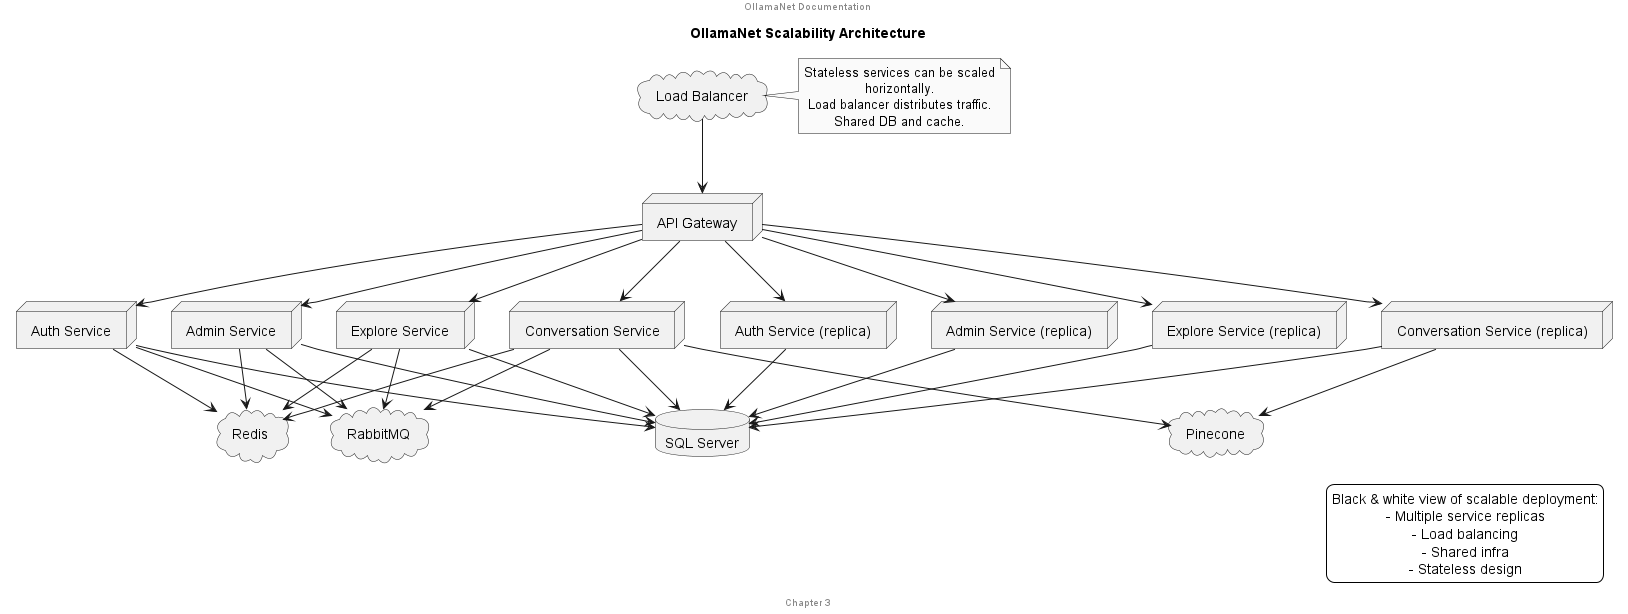
\includegraphics[width=0.8\textwidth]{./Chapter03/figures/Scalability_Architecture.png}
    \caption{OllamaNet Scalability Architecture}
    \label{fig:scalability-architecture}
\end{figure}

\subsection{Security Requirements}

The OllamaNet platform must comply with the following security requirements:

\begin{enumerate}
   \item \textbf{Authentication and Authorization}
   \begin{itemize}
      \item NFR-SEC-01: User passwords shall be stored using industry-standard hashing algorithms (bcrypt)
      \item NFR-SEC-02: JWT tokens shall expire after 15 minutes of inactivity
      \item NFR-SEC-03: Refresh tokens shall expire after 30 days
      \item NFR-SEC-04: Failed login attempts shall be limited to prevent brute force attacks
      \item NFR-SEC-05: Role-based access control shall be enforced for all protected resources
   \end{itemize}

   \item \textbf{Data Protection}
   \begin{itemize}
      \item NFR-SEC-06: All communications shall use TLS 1.3 or higher
      \item NFR-SEC-07: Sensitive data shall be encrypted at rest using AES-256
      \item NFR-SEC-08: Database credentials shall be stored in secure environment variables
      \item NFR-SEC-09: Production environments shall enforce strict network isolation
      \item NFR-SEC-10: Data access shall follow the principle of least privilege
   \end{itemize}

   \item \textbf{API Security}
   \begin{itemize}
      \item NFR-SEC-11: APIs shall validate all inputs to prevent injection attacks
      \item NFR-SEC-12: CORS policies shall restrict access to approved origins
      \item NFR-SEC-13: API endpoints shall implement rate limiting
      \item NFR-SEC-14: Error responses shall not expose implementation details
      \item NFR-SEC-15: API security headers shall be implemented (HSTS, X-XSS-Protection, etc.)
   \end{itemize}

   \item \textbf{Audit and Compliance}
   \begin{itemize}
      \item NFR-SEC-16: Security-related events shall be logged with appropriate details
      \item NFR-SEC-17: Audit logs shall be immutable and tamper-evident
      \item NFR-SEC-18: The platform shall support regulatory compliance reporting
      \item NFR-SEC-19: Privileged operations shall require additional authentication
      \item NFR-SEC-20: Regular security assessments shall be supported
   \end{itemize}

   \item \textbf{Vulnerability Management}
   \begin{itemize}
      \item NFR-SEC-21: The platform shall not use components with known vulnerabilities
      \item NFR-SEC-22: The platform shall be designed to mitigate OWASP Top 10 vulnerabilities
      \item NFR-SEC-23: Security patches shall be applicable without service interruption
      \item NFR-SEC-24: Dependencies shall be regularly updated to address security issues
      \item NFR-SEC-25: Security testing shall be integrated into the development process
   \end{itemize}
\end{enumerate}

\subsection{Reliability and Availability Requirements}

The OllamaNet platform must meet the following reliability and availability requirements:

\begin{enumerate}
   \item \textbf{System Availability}
   \begin{itemize}
      \item NFR-REL-01: The platform shall maintain 99.9\% uptime (excluding planned maintenance)
      \item NFR-REL-02: Planned maintenance shall occur during off-peak hours
      \item NFR-REL-03: No single point of failure shall exist in the production environment
      \item NFR-REL-04: The system shall support rolling updates without downtime
      \item NFR-REL-05: The platform shall detect and restart failed service instances automatically
   \end{itemize}

   \item \textbf{Fault Tolerance}
   \begin{itemize}
      \item NFR-REL-06: The platform shall implement circuit breakers for external service calls
      \item NFR-REL-07: Services shall fail gracefully when dependencies are unavailable
      \item NFR-REL-08: The system shall implement retry logic with exponential backoff
      \item NFR-REL-09: The platform shall maintain data integrity during partial system failures
      \item NFR-REL-10: The system shall recover automatically from most failure scenarios
   \end{itemize}

   \item \textbf{Data Reliability}
   \begin{itemize}
      \item NFR-REL-11: The database shall use transaction isolation to prevent data corruption
      \item NFR-REL-12: The platform shall implement data backups with point-in-time recovery
      \item NFR-REL-13: Data integrity constraints shall be enforced at the database level
      \item NFR-REL-14: The system shall detect and log data inconsistencies
      \item NFR-REL-15: Critical data changes shall be audited with before/after values
   \end{itemize}

   \item \textbf{Disaster Recovery}
   \begin{itemize}
      \item NFR-REL-16: The platform shall support database failover to standby replicas
      \item NFR-REL-17: Recovery Point Objective (RPO) shall be less than 5 minutes
      \item NFR-REL-18: Recovery Time Objective (RTO) shall be less than 30 minutes
      \item NFR-REL-19: Disaster recovery procedures shall be documented and tested
      \item NFR-REL-20: The system shall support geographic redundancy for critical components
   \end{itemize}
\end{enumerate}

\subsection{Maintainability Requirements}

The OllamaNet platform must adhere to the following maintainability requirements:

\begin{enumerate}
   \item \textbf{Code Quality}
   \begin{itemize}
      \item NFR-MAIN-01: Code shall follow language-specific style guidelines
      \item NFR-MAIN-02: Code complexity metrics shall remain below specified thresholds
      \item NFR-MAIN-03: Test coverage shall exceed 80\% for critical components
      \item NFR-MAIN-04: Static code analysis shall be part of the build process
      \item NFR-MAIN-05: Code shall be properly commented and documented
   \end{itemize}

   \item \textbf{Deployment}
   \begin{itemize}
      \item NFR-MAIN-06: The platform shall support containerized deployment
      \item NFR-MAIN-07: Configuration shall be externalized from code
      \item NFR-MAIN-08: The system shall support environment-specific configuration
      \item NFR-MAIN-09: Deployment shall be automated via CI/CD pipelines
      \item NFR-MAIN-10: Deployments shall be reversible through rollback mechanisms
   \end{itemize}

   \item \textbf{Monitoring and Diagnostics}
   \begin{itemize}
      \item NFR-MAIN-11: Services shall expose health check endpoints
      \item NFR-MAIN-12: The system shall generate appropriate logs for troubleshooting
      \item NFR-MAIN-13: Performance metrics shall be collected and available for analysis
      \item NFR-MAIN-14: Error conditions shall trigger appropriate alerts
      \item NFR-MAIN-15: The platform shall support distributed tracing
   \end{itemize}

   \item \textbf{Extensibility}
   \begin{itemize}
      \item NFR-MAIN-16: The system architecture shall support adding new services
      \item NFR-MAIN-17: APIs shall be versioned to support evolution
      \item NFR-MAIN-18: The database schema shall support extension without redesign
      \item NFR-MAIN-19: User interface components shall be modular and reusable
      \item NFR-MAIN-20: The system shall support plugin architectures where appropriate
   \end{itemize}
\end{enumerate}

\subsection{Compatibility and Interoperability Requirements}

The OllamaNet platform must satisfy the following compatibility and interoperability requirements:

\begin{enumerate}
   \item \textbf{Client Compatibility}
   \begin{itemize}
      \item NFR-COMP-01: Frontend applications shall work on modern browsers (Chrome, Firefox, Safari, Edge)
      \item NFR-COMP-02: The system shall support responsive design for mobile and desktop access
      \item NFR-COMP-03: APIs shall be accessible from common programming languages
      \item NFR-COMP-04: The platform shall support common authentication mechanisms (JWT, OAuth)
      \item NFR-COMP-05: Public interfaces shall follow industry standards for maximum compatibility
   \end{itemize}

   \item \textbf{Integration Compatibility}
   \begin{itemize}
      \item NFR-COMP-06: The platform shall use standard protocols for integration (REST, AMQP)
      \item NFR-COMP-07: Data exchange shall use standardized formats (JSON, XML)
      \item NFR-COMP-08: APIs shall provide Swagger/OpenAPI documentation
      \item NFR-COMP-09: The platform shall support standard database connection mechanisms
      \item NFR-COMP-10: Integration points shall be well documented for third-party developers
   \end{itemize}

   \item \textbf{Environment Compatibility}
   \begin{itemize}
      \item NFR-COMP-11: The platform shall operate in common cloud environments (AWS, Azure, GCP)
      \item NFR-COMP-12:
</rewritten_file>






\cleardoublepage
\def\chapdir{./Chapter04}

\chapter{System Architecture} \label{ch:system-architecture}

\section{Overall Architecture}

\subsection{High-level System Architecture Overview}

The OllamaNet platform is built on a modern microservices architecture that separates concerns into distinct, independently deployable services. Each service focuses on a specific domain within the system, communicating through well-defined APIs and messaging patterns.

\begin{figure}[p]
    \centering
    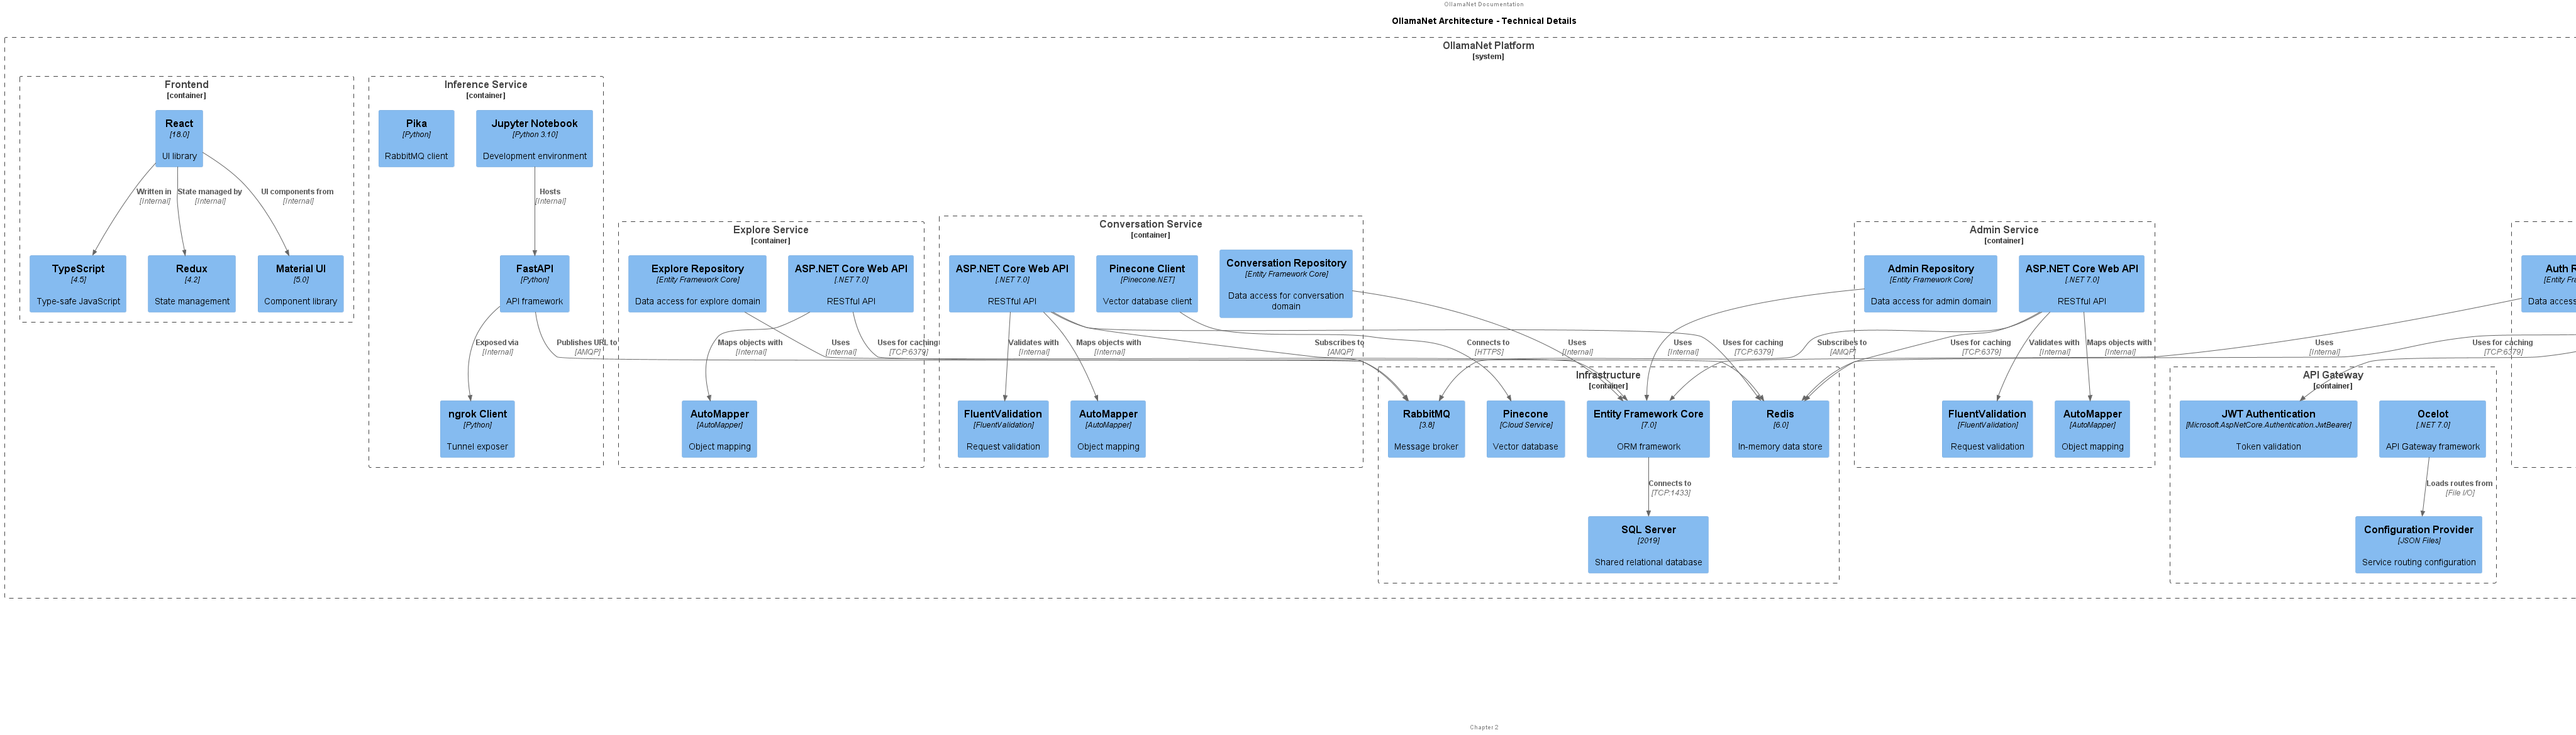
\includegraphics[width=\textwidth]{./Chapter04/figures/OllamaNet_Architecture.png}
    \caption{OllamaNet High-level System Architecture}
    \label{fig:system-architecture}
\end{figure}
\clearpage

The architecture consists of the following key components:

\begin{enumerate}
   \item \textbf{API Gateway}: Serves as the entry point for all client requests, handling routing, authentication, and cross-cutting concerns.
   \item \textbf{Auth Service}: Manages user authentication, authorization, and account management.
   \item \textbf{Admin Service}: Provides administrative capabilities for user and model management.
   \item \textbf{Explore Service}: Enables discovery and browsing of available AI models.
   \item \textbf{Conversation Service}: Handles conversation management and interaction with AI models.
   \item \textbf{Inference Service}: Connects to the Ollama engine for AI model inference.
   \item \textbf{Database Layer}: Provides data persistence across services.
   \item \textbf{RabbitMQ}: Facilitates asynchronous communication and service discovery.
\end{enumerate}

\subsection{Architectural Principles and Goals}

The OllamaNet architecture adheres to the following principles:

\begin{enumerate}
   \item \textbf{Service Independence}: Each service can be developed, deployed, and scaled independently.
   \item \textbf{Domain-Driven Design}: Services are organized around business domains rather than technical functions.
   \item \textbf{API-First Design}: All services expose well-defined APIs with consistent patterns.
   \item \textbf{Resilience by Design}: The system is designed to handle failures gracefully.
   \item \textbf{Security at Every Layer}: Authentication and authorization are enforced consistently.
   \item \textbf{Scalability}: Services can be scaled independently based on demand.
   \item \textbf{Observability}: The system provides monitoring, logging, and diagnostics capabilities.
\end{enumerate}

The architectural goals include:

\begin{enumerate}
   \item \textbf{Maintainability}: Clear separation of concerns makes the system easier to maintain.
   \item \textbf{Extensibility}: New features can be added with minimal impact on existing components.
   \item \textbf{Performance}: The architecture optimizes for responsive user experiences.
   \item \textbf{Security}: The system protects user data and prevents unauthorized access.
   \item \textbf{Reliability}: The system remains available and consistent even during partial failures.
\end{enumerate}

\subsection{System Topology and Deployment View}

The OllamaNet system is designed for flexible deployment across various environments:

\begin{sidewaysfigure}[p]
    \centering
    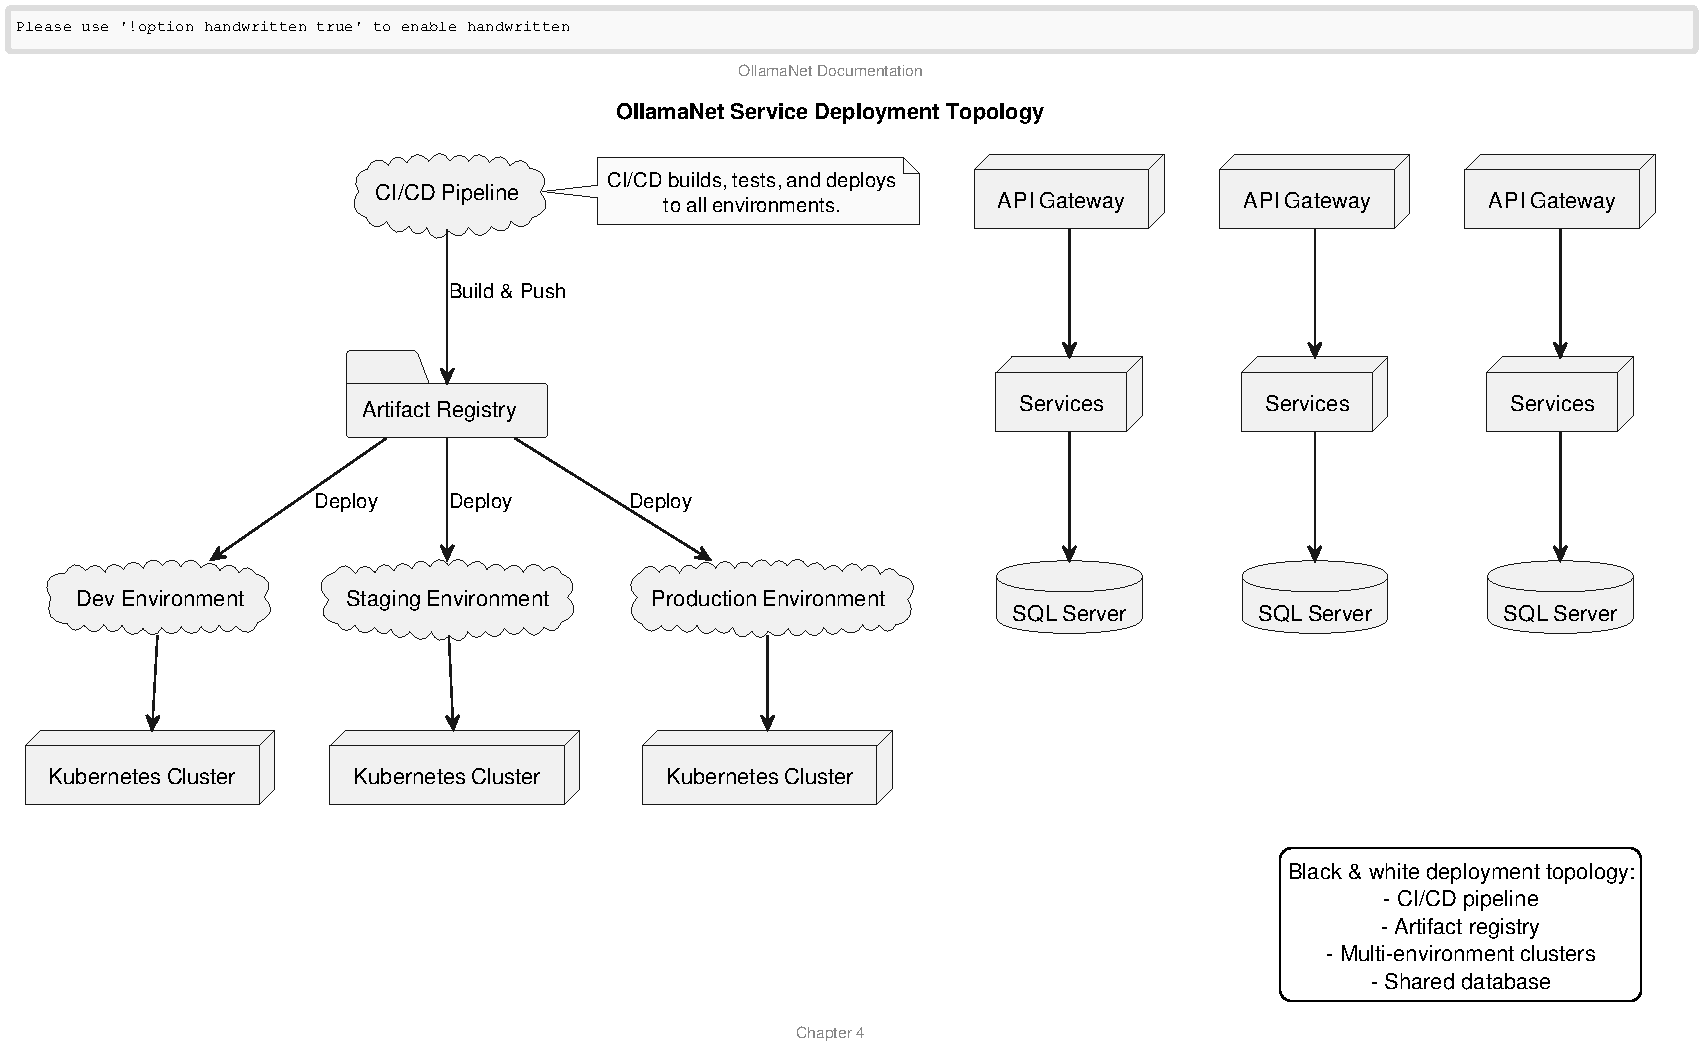
\includegraphics[width=\textwidth]{./Chapter04/figures/service_deployment.pdf}
    \caption{OllamaNet System Topology and Deployment View}
    \label{fig:system-topology}
\end{sidewaysfigure}
\clearpage

The deployment architecture supports:

\begin{enumerate}
   \item \textbf{Containerization}: All services are containerized for consistent deployment.
   \item \textbf{Horizontal Scaling}: Services can be scaled out by adding instances.
   \item \textbf{Environment Isolation}: Development, testing, and production environments are isolated.
   \item \textbf{Cloud Deployment}: The system can be deployed to various cloud providers.
   \item \textbf{On-Premises Deployment}: The system can also be deployed on-premises.
\end{enumerate}

\subsection{Key Architectural Decisions and Rationales}

\begin{table}[h]
  \centering
  \caption{Key Architectural Decisions and Rationales}
  \label{tab:architectural-decisions}
  \begin{tabular}{|p{0.3\textwidth}|p{0.6\textwidth}|}
    \hline
    \textbf{Decision} & \textbf{Rationale} \\
    \hline
    Microservices Architecture & Enables independent development, deployment, and scaling of components \\
    \hline
    API Gateway Pattern & Provides a single entry point for clients, simplifying client integration \\
    \hline
    Domain-Driven Design & Aligns services with business domains for better maintainability \\
    \hline
    JWT Authentication & Enables stateless authentication across services \\
    \hline
    SQL Server Database & Provides robust relational data storage with strong consistency \\
    \hline
    Redis Caching & Improves performance by caching frequently accessed data \\
    \hline
    RabbitMQ Messaging & Enables asynchronous communication and service discovery \\
    \hline
    Notebook-First Inference & Allows flexible deployment of inference capabilities in cloud environments \\
    \hline
  \end{tabular}
\end{table}

\section{Service Decomposition Strategy}

\subsection{Microservice Boundaries and Responsibilities}

The OllamaNet platform is decomposed into services based on business domains and responsibilities:

\begin{enumerate}
   \item \textbf{Auth Service}
   \begin{itemize}
      \item User registration and authentication
      \item JWT token issuance and validation
      \item Role and permission management
      \item User profile management
   \end{itemize}

   \item \textbf{Admin Service}
   \begin{itemize}
      \item User account administration
      \item AI model management and deployment
      \item Tag and category management
      \item System configuration and monitoring
   \end{itemize}

   \item \textbf{Explore Service}
   \begin{itemize}
      \item AI model discovery and browsing
      \item Search and filtering capabilities
      \item Model metadata presentation
      \item Caching for performance optimization
   \end{itemize}

   \item \textbf{Conversation Service}
   \begin{itemize}
      \item Conversation management and organization
      \item Chat interaction with AI models
      \item Document processing for context enhancement
      \item Folder and organization features
   \end{itemize}

   \item \textbf{Inference Service (Spicy Avocado)}
   \begin{itemize}
      \item AI model inference and response generation
      \item Service discovery via RabbitMQ
      \item Notebook-first architecture for cloud deployment
      \item Integration with Ollama engine
   \end{itemize}

   \item \textbf{Gateway Service}
   \begin{itemize}
      \item Request routing to appropriate services
      \item Authentication and authorization enforcement
      \item Cross-cutting concerns like CORS and rate limiting
      \item Request/response transformation
   \end{itemize}
\end{enumerate}

\subsection{Domain-Driven Design Application}

The service decomposition follows Domain-Driven Design principles:

\begin{enumerate}
   \item \textbf{Bounded Contexts}: Each service represents a distinct bounded context with its own domain model.
   \item \textbf{Ubiquitous Language}: Each service uses consistent terminology within its domain.
   \item \textbf{Aggregates}: Domain entities are organized into aggregates with clear boundaries.
   \item \textbf{Domain Events}: Services communicate through domain events when appropriate.
\end{enumerate}

\begin{sidewaysfigure}[p]
    \centering
    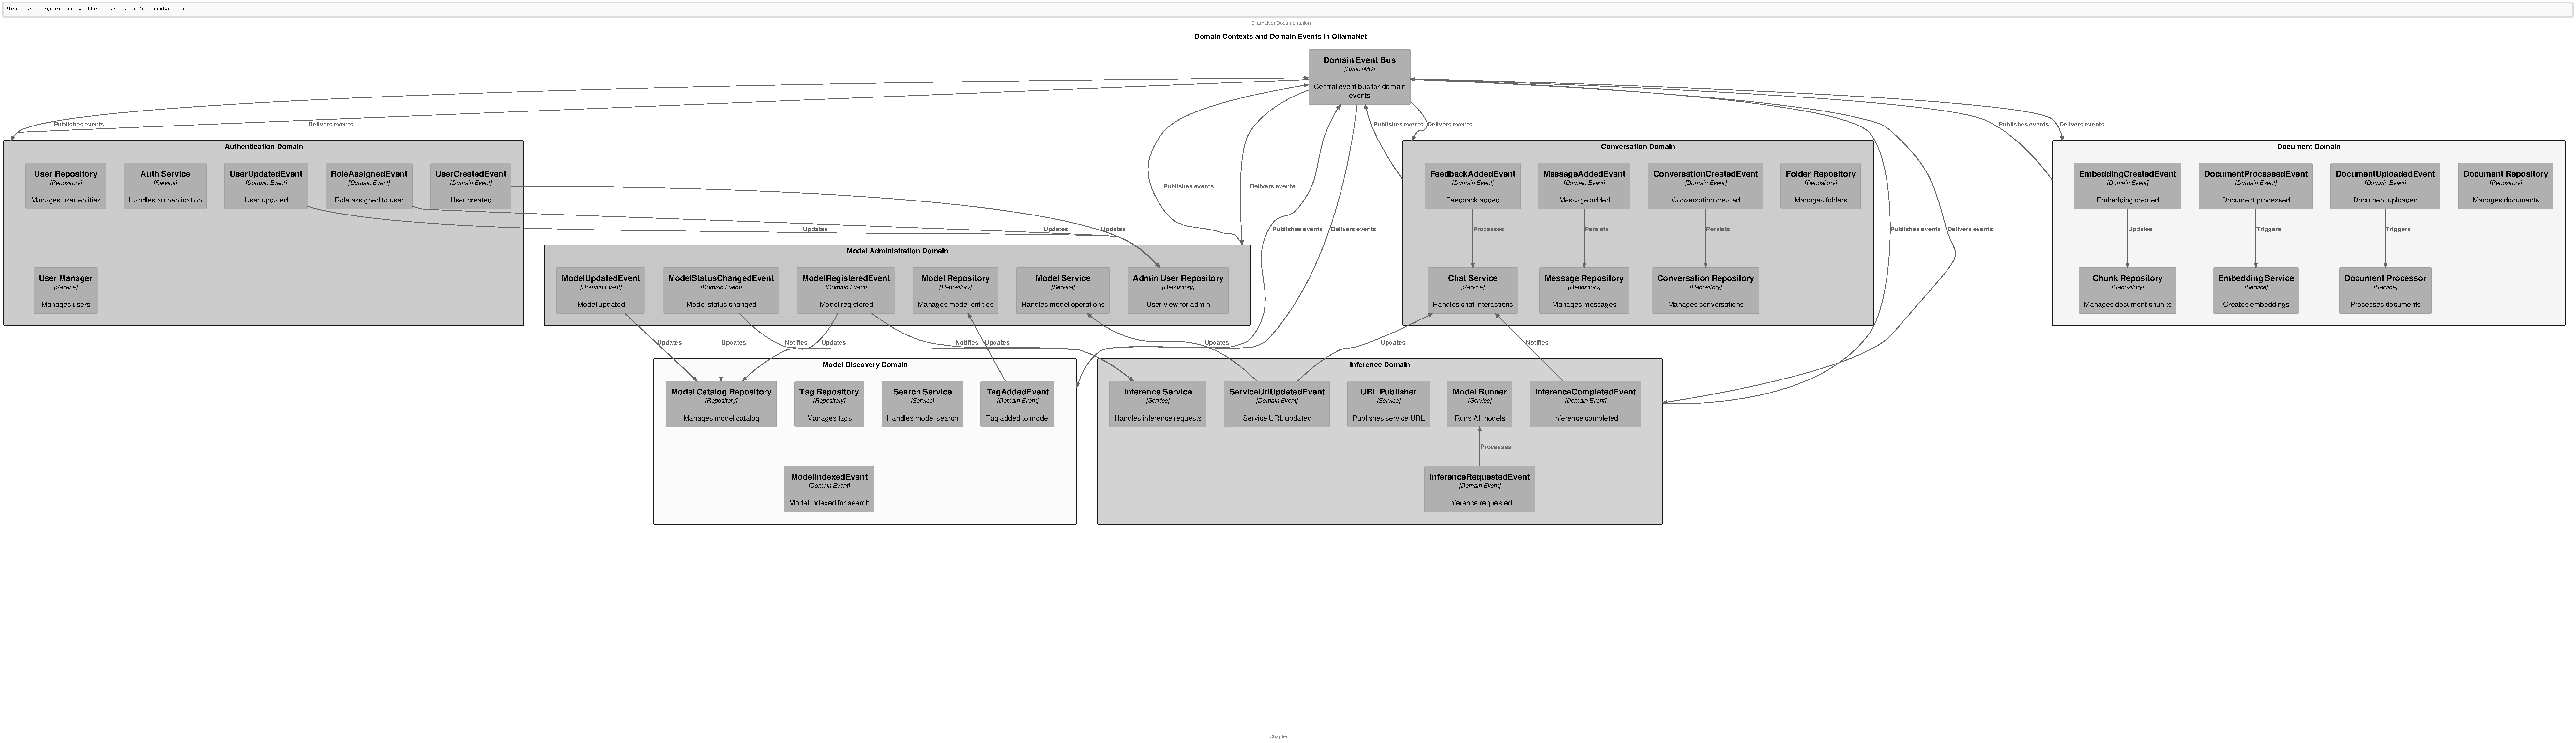
\includegraphics[width=\textwidth]{./Chapter04/figures/domain_contexts.pdf}
    \caption{OllamaNet Bounded Contexts in Domain-Driven Design}
    \label{fig:domain-contexts}
\end{sidewaysfigure}
\clearpage

\subsection{Service Granularity Decisions}

The service granularity in OllamaNet balances several factors:

\begin{enumerate}
   \item \textbf{Business Domain Alignment}: Services align with distinct business capabilities.
   \item \textbf{Team Ownership}: Services can be owned by specific teams.
   \item \textbf{Deployment Independence}: Services can be deployed independently.
   \item \textbf{Scalability Requirements}: Services can be scaled based on their specific load patterns.
\end{enumerate}

For example, the Inference Service is separated from the Conversation Service because:
\begin{itemize}
   \item It has different scaling requirements (compute-intensive)
   \item It has a unique deployment model (notebook-first architecture)
   \item It integrates with external systems (Ollama engine)
\end{itemize}

\subsection{Service Composition and Dependencies}

Services in OllamaNet have the following dependencies:

\begin{enumerate}
   \item \textbf{Auth Service}: No dependencies on other services
   \item \textbf{Admin Service}: Depends on Auth Service for authentication
   \item \textbf{Explore Service}: Depends on Auth Service for authentication
   \item \textbf{Conversation Service}: 
   \begin{itemize}
      \item Depends on Auth Service for authentication
      \item Depends on Inference Service for AI model responses
   \end{itemize}
   \item \textbf{Inference Service}: No direct dependencies on other services
   \item \textbf{Gateway Service}: Depends on all services for routing
\end{enumerate}

\begin{sidewaysfigure}[p]
    \centering
    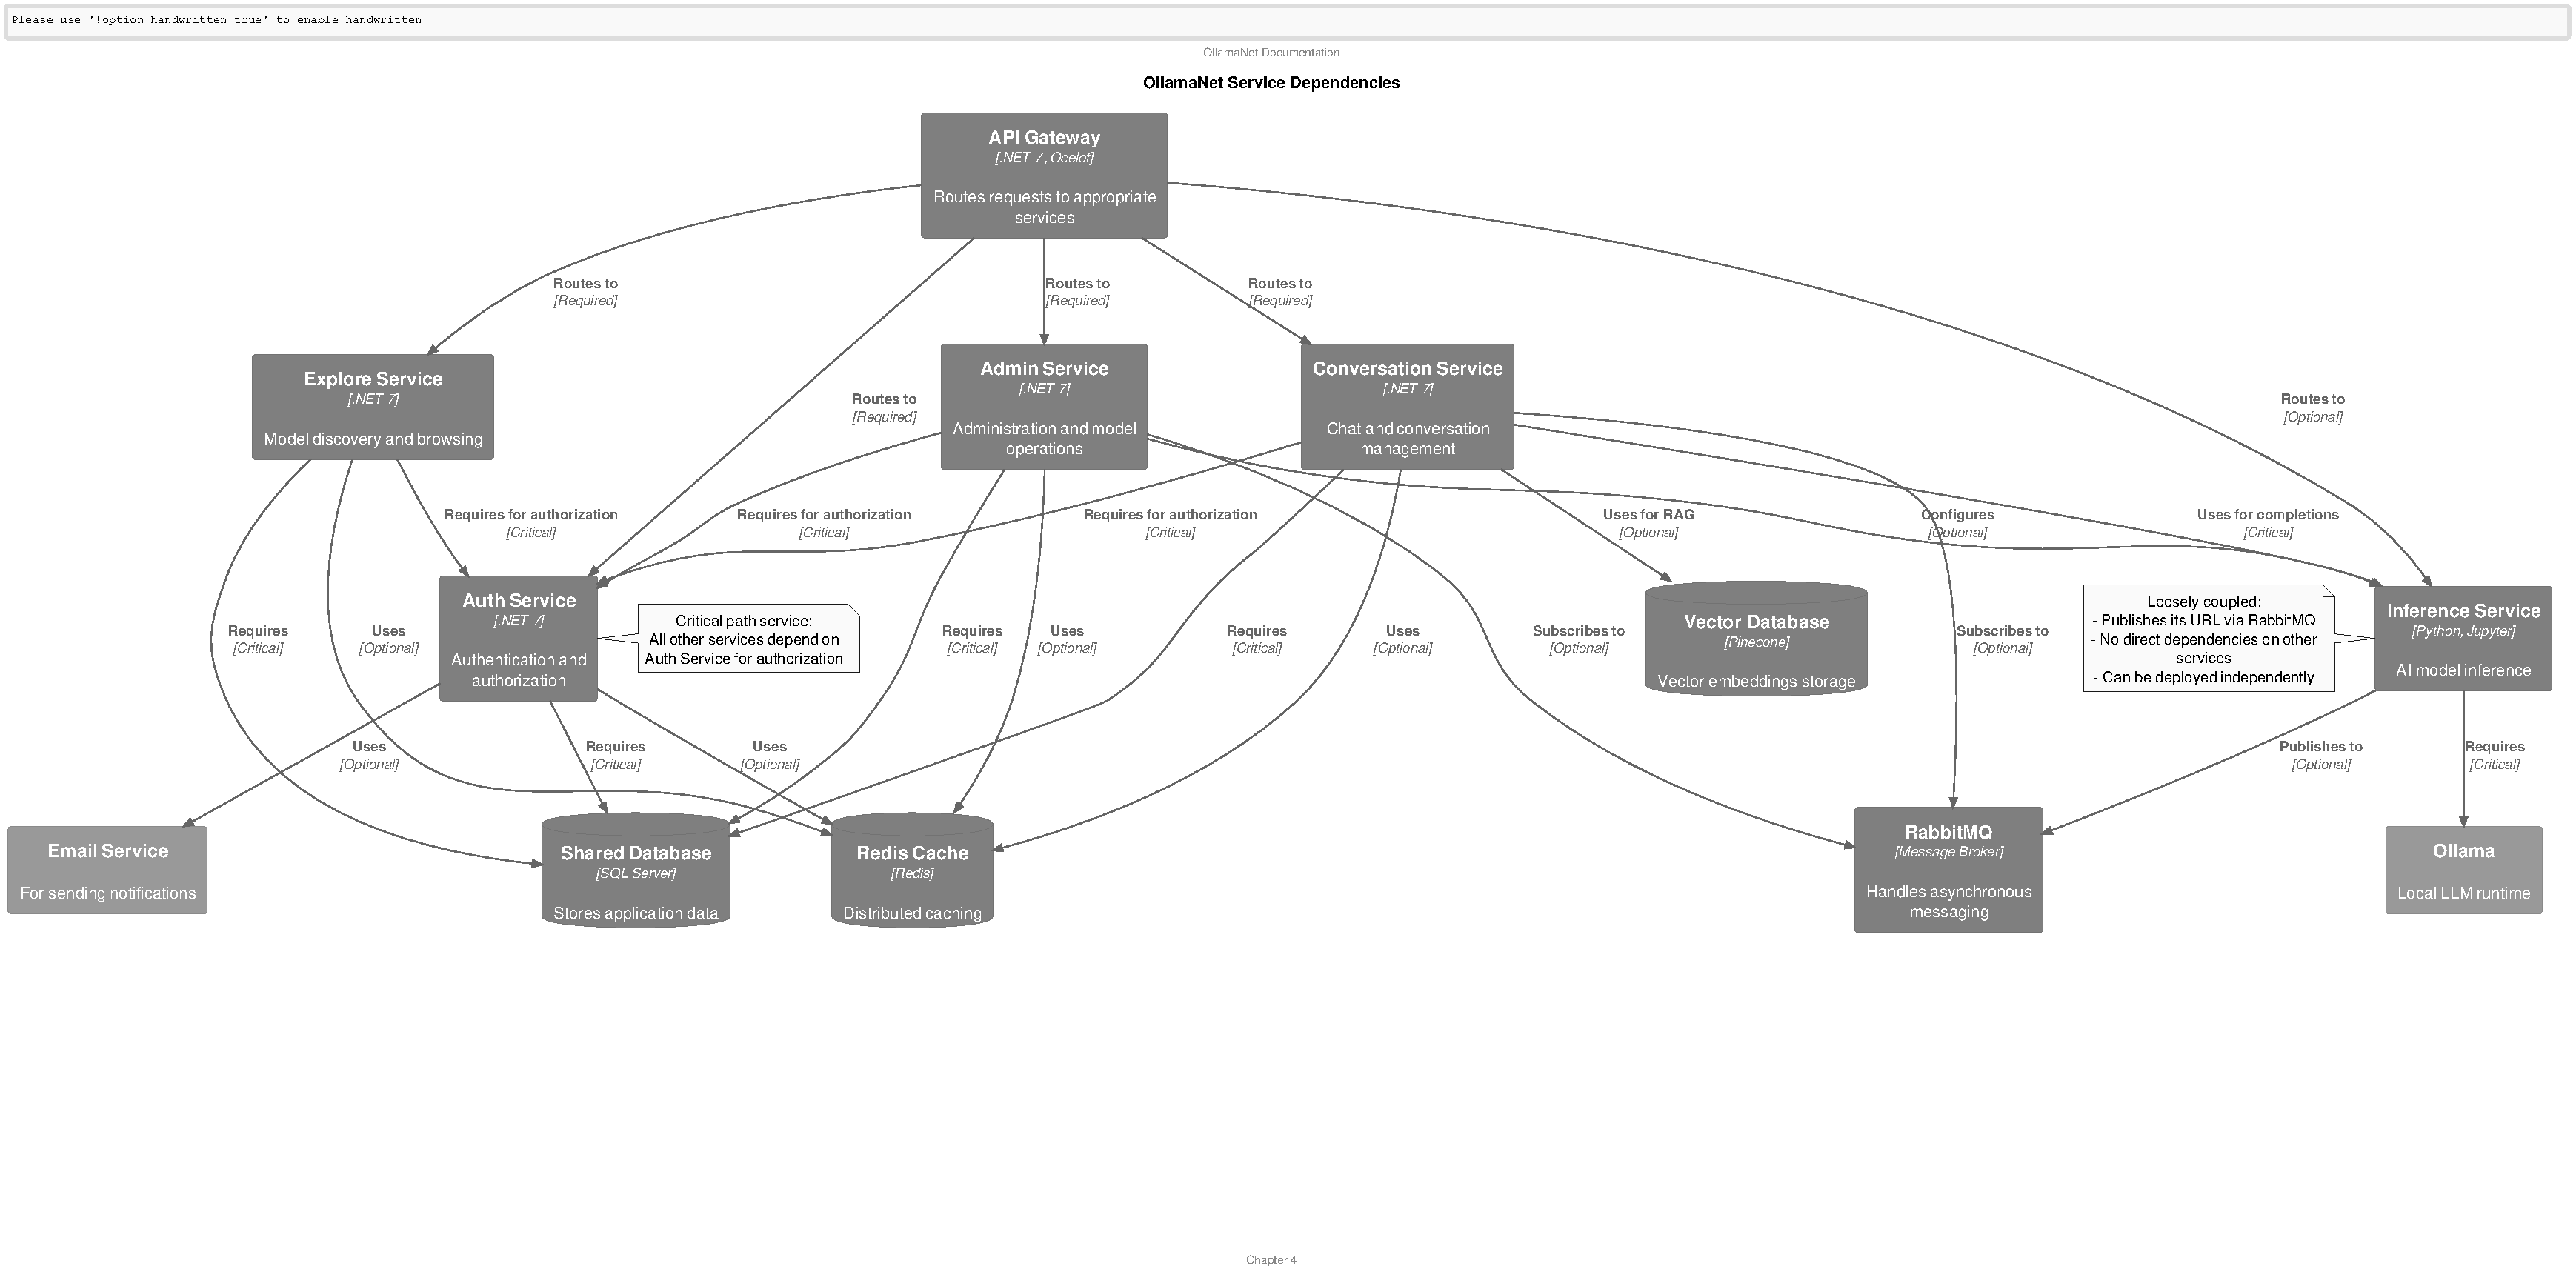
\includegraphics[width=\textwidth]{./Chapter04/figures/service_dependencies.pdf}
    \caption{OllamaNet Service Dependencies}
    \label{fig:service-dependencies}
\end{sidewaysfigure}
\clearpage

\section{Service Discovery and Registry}

\subsection{Service Discovery Mechanisms}

OllamaNet implements service discovery using RabbitMQ, particularly for the dynamic discovery of Inference Service endpoints:

\begin{enumerate}
   \item \textbf{Publisher-Subscriber Pattern}: Services publish their endpoints to RabbitMQ topics.
   \item \textbf{Topic Exchange}: A "service-discovery" exchange routes messages based on routing keys.
   \item \textbf{Routing Keys}: Structured keys like "inference.url.changed" identify message types.
   \item \textbf{Message Format}: JSON messages contain service URLs and metadata.
\end{enumerate}

\begin{sidewaysfigure}[p]
    \centering
    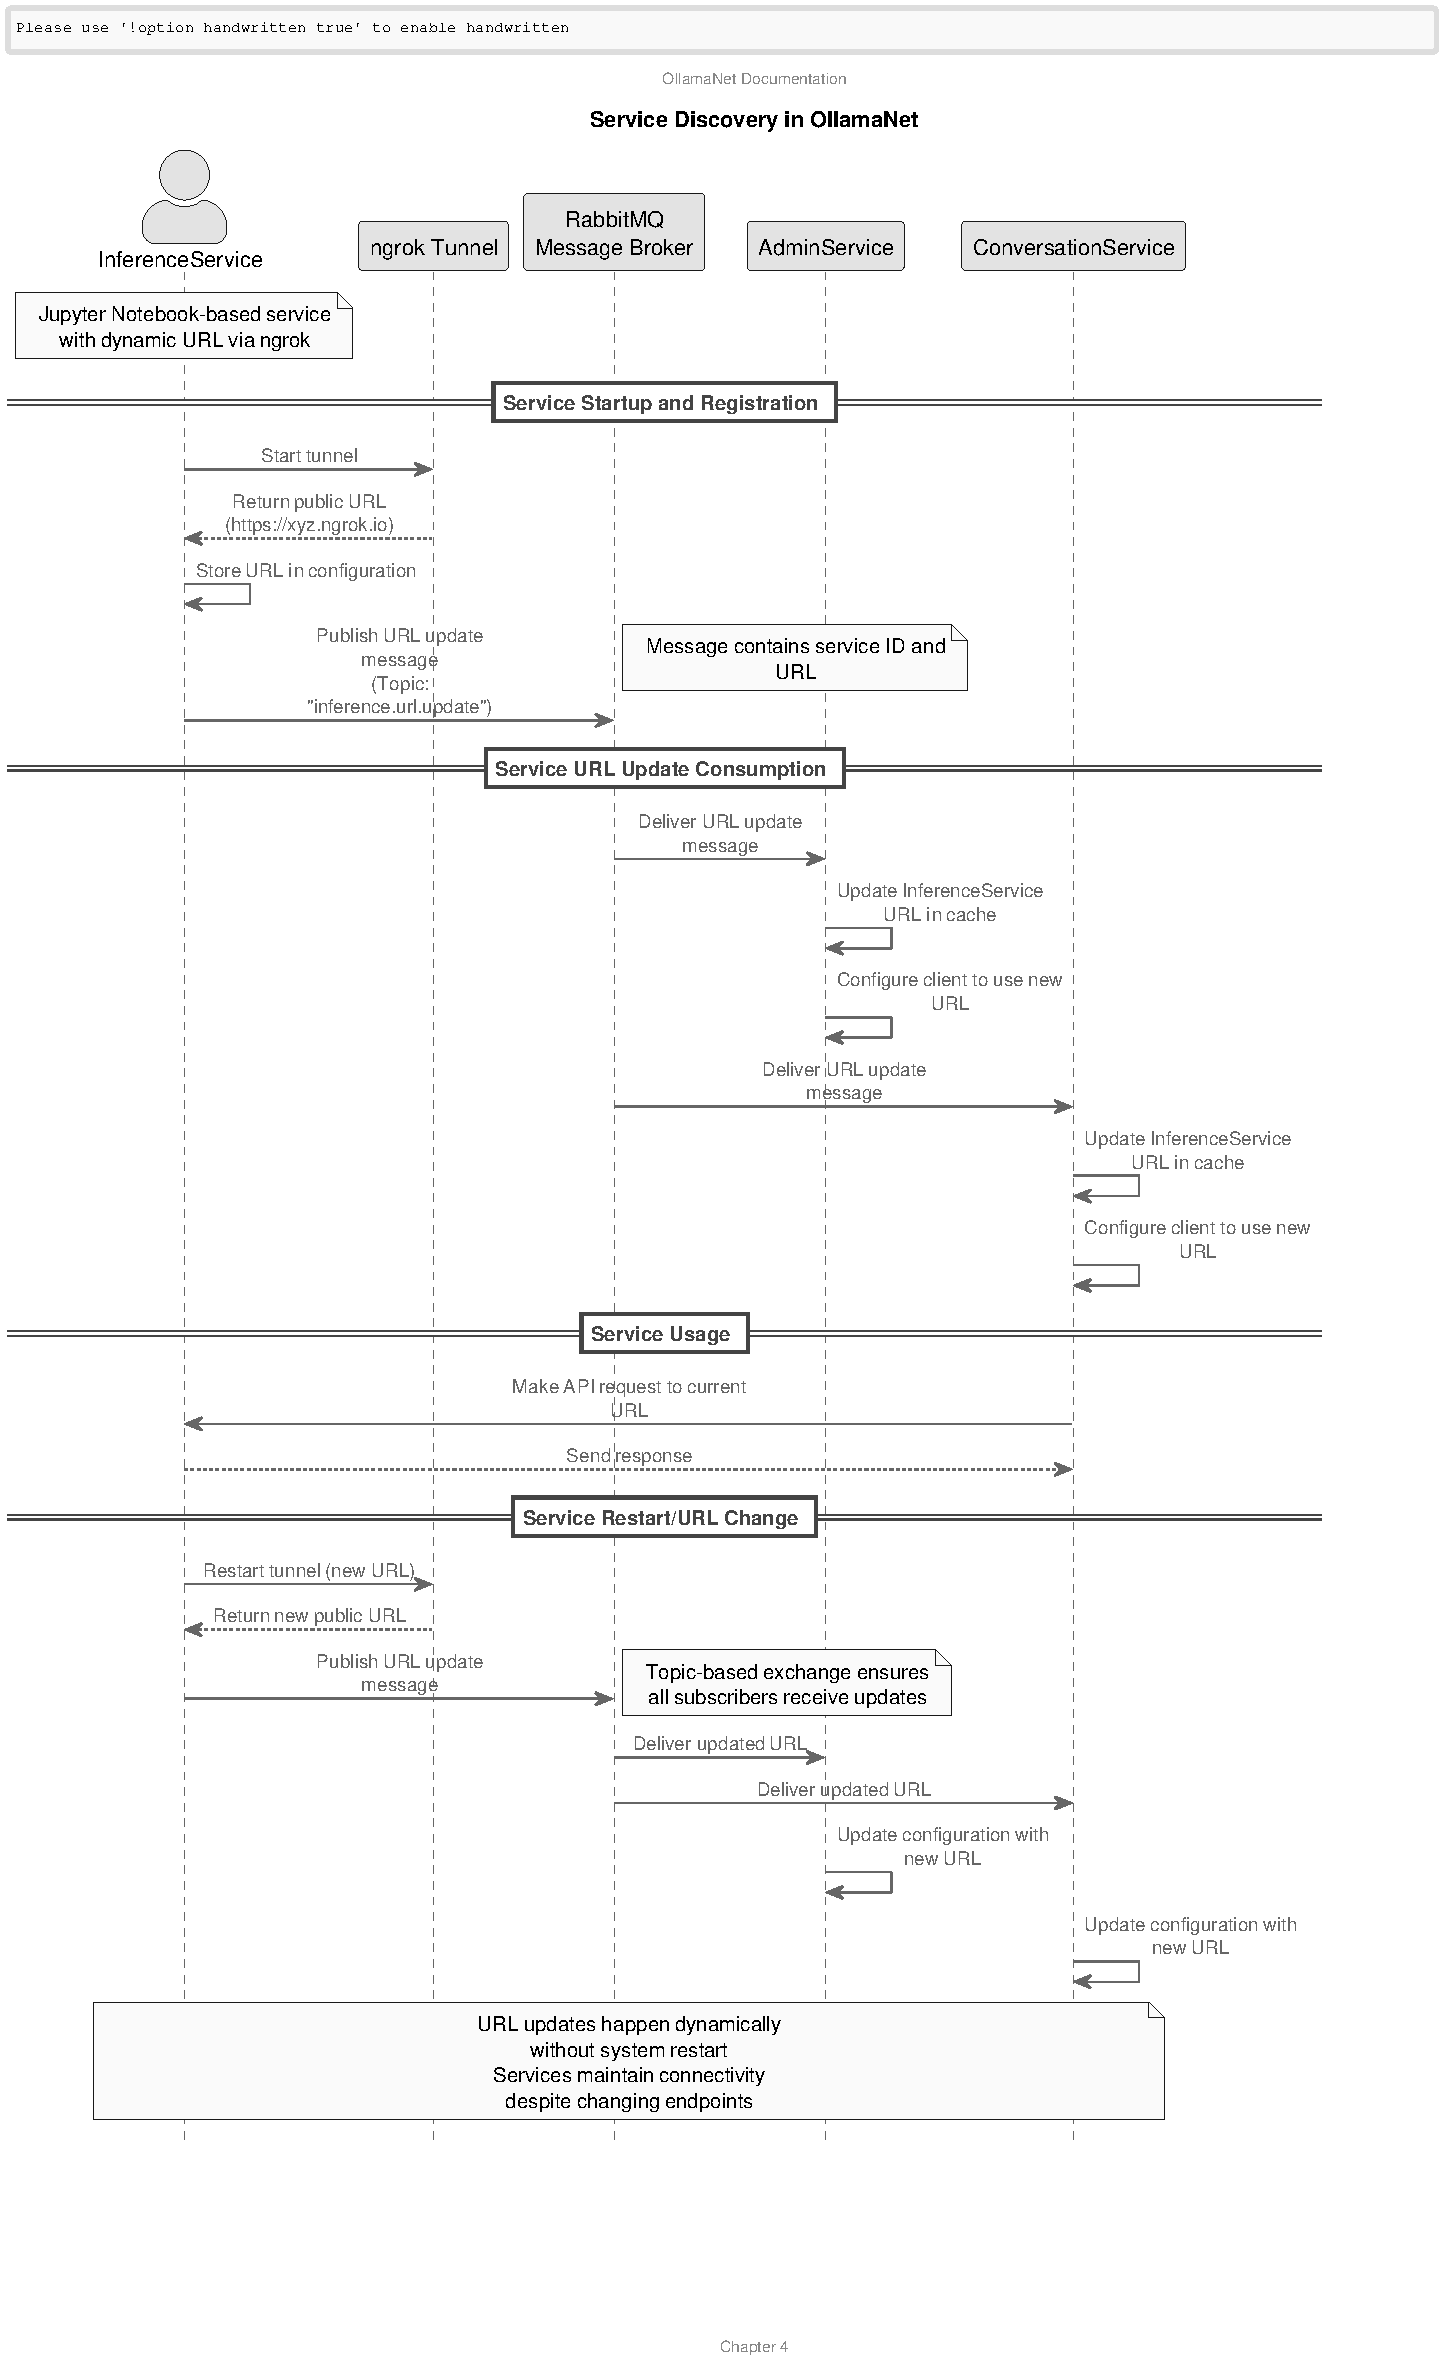
\includegraphics[width=\textwidth]{./Chapter04/figures/service_discovery.pdf}
    \caption{Service Discovery Sequence Diagram}
    \label{fig:service-discovery}
\end{sidewaysfigure}
\clearpage

\subsection{Dynamic Service URL Configuration}

The system handles dynamic URL configuration through several mechanisms:

\begin{enumerate}
   \item \textbf{Initial Configuration}: Services start with default URLs from configuration files.
   \item \textbf{Runtime Updates}: Services receive URL updates via RabbitMQ messages.
   \item \textbf{Configuration Service}: A central service manages and distributes configuration.
   \item \textbf{Caching}: Updated URLs are cached in Redis for persistence across restarts.
\end{enumerate}

\begin{verbatim}
public async Task UpdateBaseUrl(string newUrl)
{
    if (string.IsNullOrEmpty(newUrl) || _currentBaseUrl == newUrl)
        return;
        
    if (!_urlValidator.IsValid(newUrl))
    {
        _logger.LogWarning("Received invalid URL update: {Url}", newUrl);
        return;
    }
    
    _currentBaseUrl = newUrl;
    await _redisCacheService.SetStringAsync(CACHE_KEY, newUrl);
    _logger.LogInformation("InferenceEngine URL updated to: {Url}", newUrl);
    
    BaseUrlChanged?.Invoke(newUrl);
}
\end{verbatim}

\subsection{Service Registration Approaches}

Services register themselves through different mechanisms:

\begin{enumerate}
   \item \textbf{Static Registration}: Most services have static endpoints defined in configuration.
   \item \textbf{Dynamic Registration}: The Inference Service dynamically registers its endpoint.
   \item \textbf{Health Checks}: Services provide health check endpoints for availability monitoring.
   \item \textbf{Service Metadata}: Registration includes service metadata like version and capabilities.
\end{enumerate}

\subsection{Service Health Monitoring}

The system monitors service health through several approaches:

\begin{enumerate}
   \item \textbf{Health Check Endpoints}: Each service exposes a \texttt{/health} endpoint.
   \item \textbf{Circuit Breakers}: Services implement circuit breakers to detect and handle failures.
   \item \textbf{Heartbeats}: Services send periodic heartbeats to indicate liveness.
   \item \textbf{Logging and Monitoring}: Centralized logging captures service health events.
\end{enumerate}

\section{API Gateway}

\subsection{Gateway Architecture Using Ocelot}

The OllamaNet Gateway is built using the Ocelot API Gateway library, providing a robust and flexible routing solution:

\begin{sidewaysfigure}[p]
    \centering
    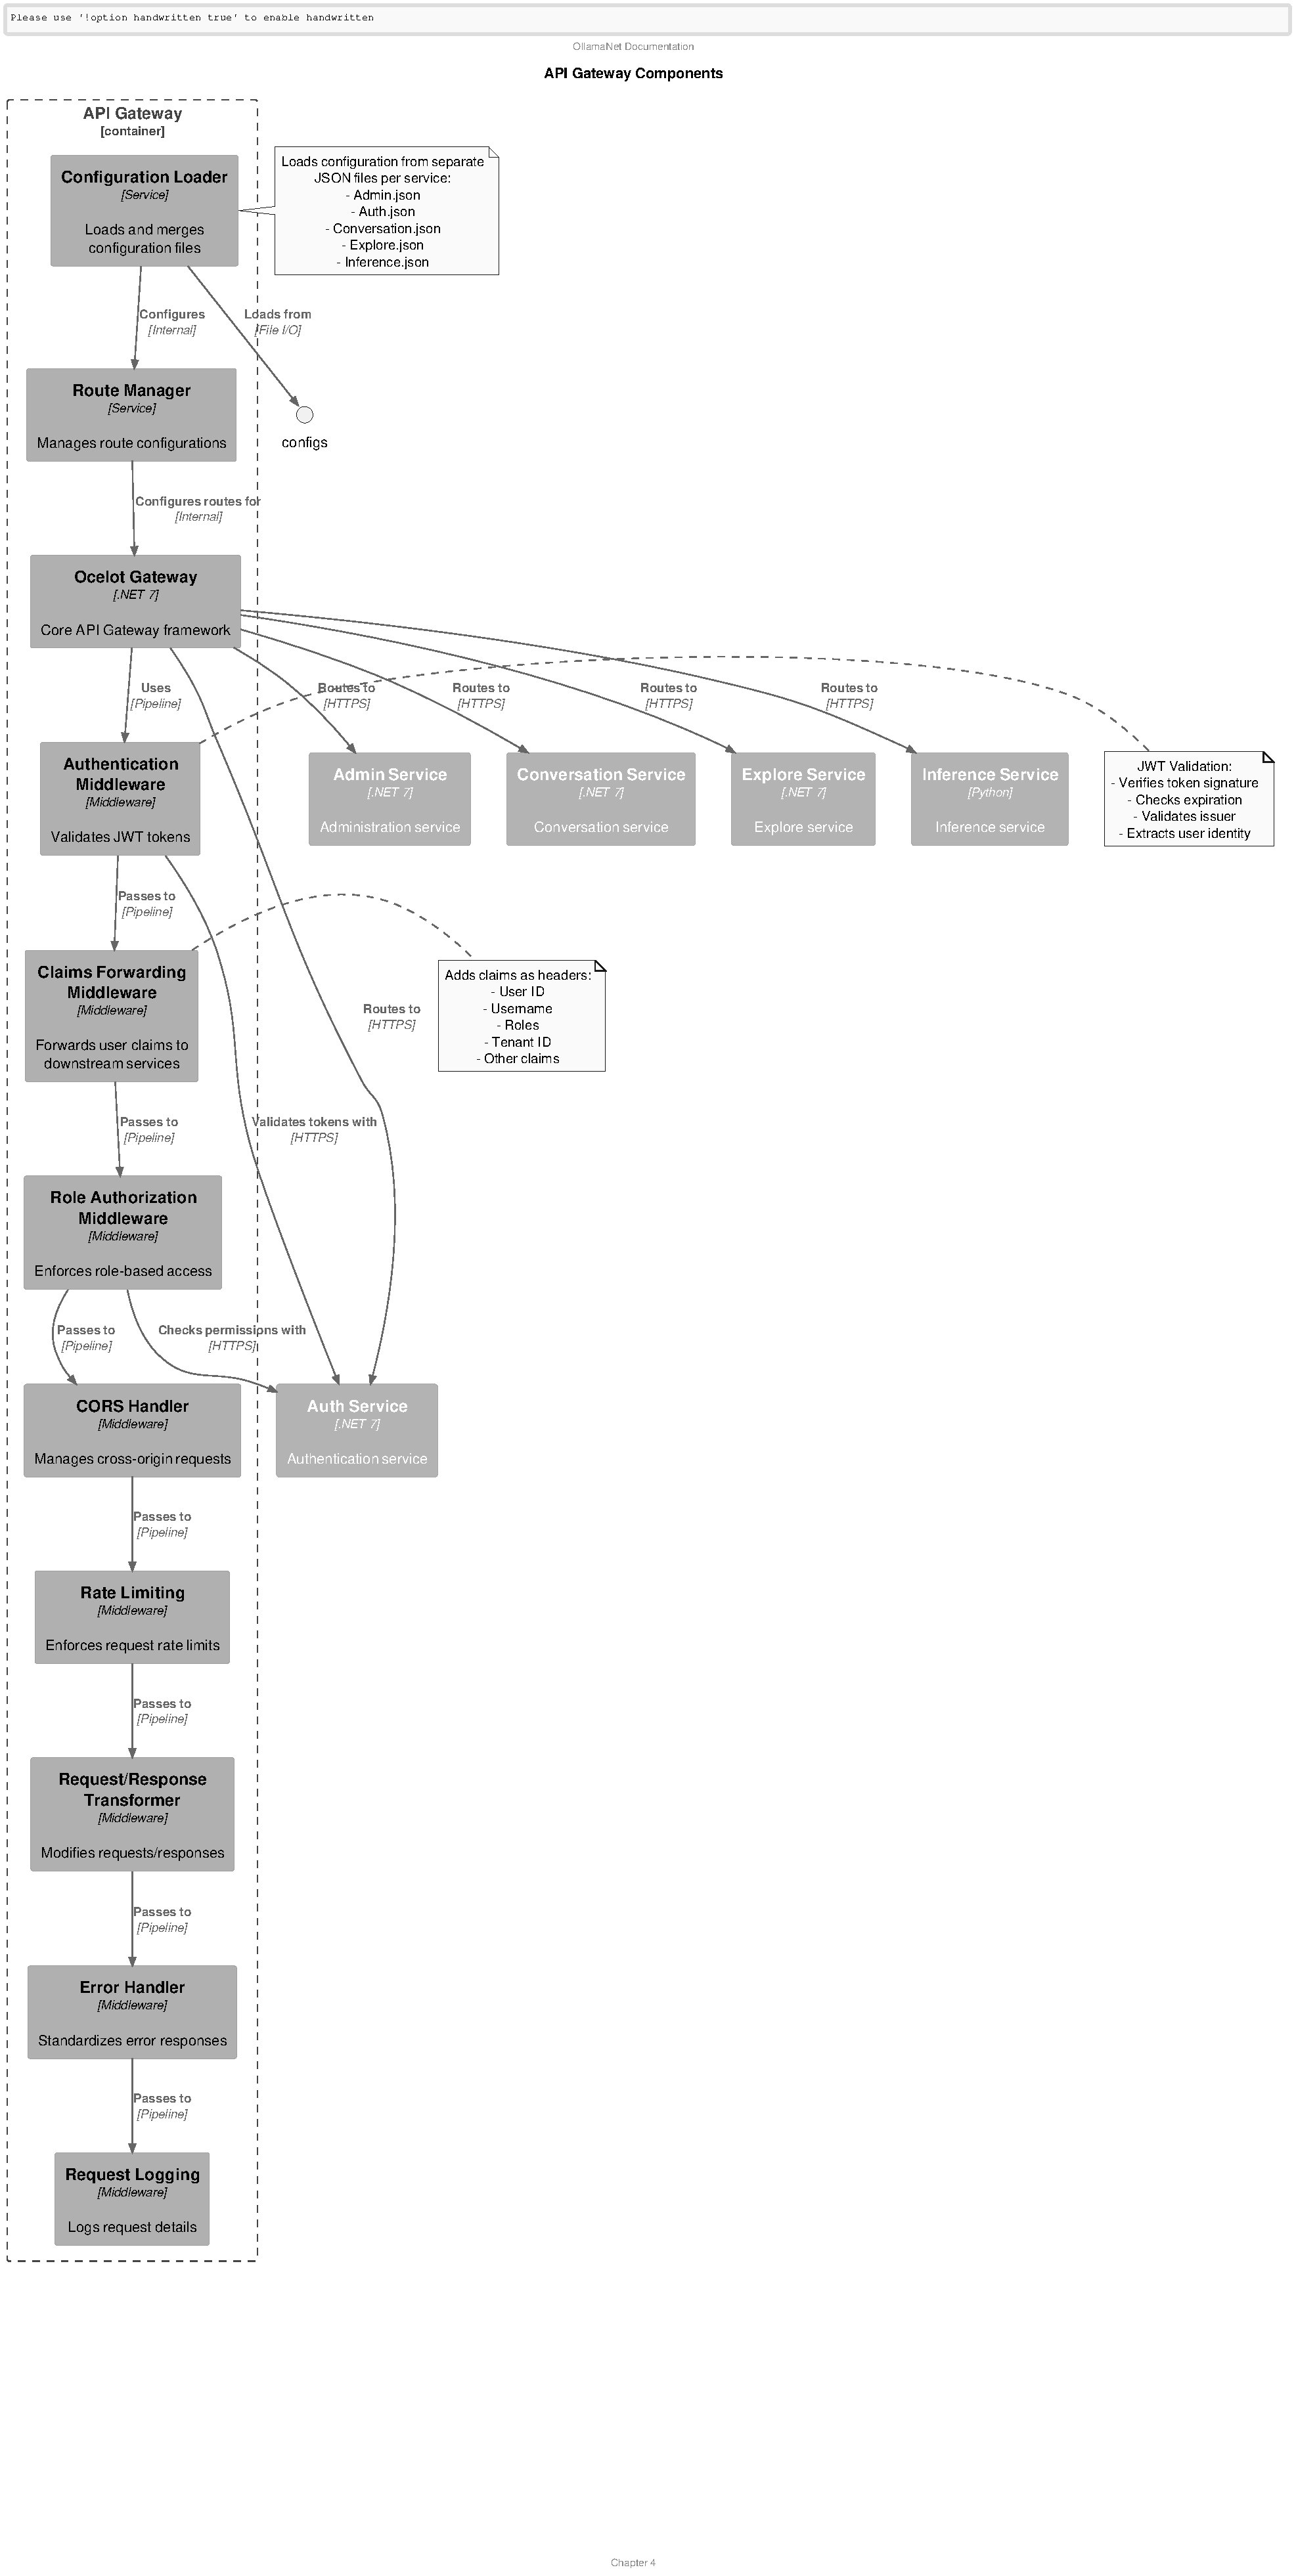
\includegraphics[width=\textwidth]{./Chapter04/figures/gateway_components.pdf}
    \caption{Gateway Architecture Components}
    \label{fig:gateway-components}
\end{sidewaysfigure}
\clearpage

Key components of the Gateway architecture include:

\begin{enumerate}
   \item \textbf{Ocelot Core}: Handles request routing based on configuration.
   \item \textbf{Middleware Pipeline}: Processes requests through a series of middleware components.
   \item \textbf{Configuration System}: Manages routing and other gateway settings.
   \item \textbf{Authentication Integration}: Validates JWT tokens and enforces security.
\end{enumerate}

\subsection{Routing Configuration and Management}

The Gateway uses a modular configuration approach:

\begin{enumerate}
   \item \textbf{Service-Specific Configurations}: Each service has its own configuration file.
   \item \textbf{Variable Substitution}: Service URLs are defined centrally and referenced via variables.
   \item \textbf{Dynamic Reloading}: Configuration changes are detected and applied without restart.
   \item \textbf{Aggregation}: Individual configurations are combined at runtime.
\end{enumerate}

\begin{verbatim}
{
  "Routes": [
    {
      "DownstreamPathTemplate": "/api/auth/{everything}",
      "DownstreamScheme": "https",
      "DownstreamHostAndPorts": [
        {
          "Host": "${Services.Auth.Host}",
          "Port": 443
        }
      ],
      "UpstreamPathTemplate": "/api/auth/{everything}",
      "UpstreamHttpMethod": [ "GET", "POST", "PUT", "DELETE" ]
    }
  ]
}
\end{verbatim}

\subsection{Authentication and Authorization at Gateway Level}

The Gateway handles authentication and authorization through:

\begin{enumerate}
   \item \textbf{JWT Validation}: Validates tokens issued by the Auth Service.
   \item \textbf{Role-Based Authorization}: Enforces access control based on user roles.
   \item \textbf{Claims Forwarding}: Extracts user claims and forwards them to downstream services.
   \item \textbf{Centralized Policy Enforcement}: Applies consistent security policies across all services.
\end{enumerate}

\begin{verbatim}
public async Task InvokeAsync(HttpContext context)
{
    if (context.User.Identity?.IsAuthenticated ?? false)
    {
        // Extract claims from the authenticated user
        var userId = context.User.FindFirst(ClaimTypes.NameIdentifier)?.Value;
        var email = context.User.FindFirst(ClaimTypes.Email)?.Value;
        var roles = context.User.FindAll(ClaimTypes.Role).Select(c => c.Value);
        
        // Add claims as headers to the request
        if (!string.IsNullOrEmpty(userId))
            context.Request.Headers.Add("X-User-Id", userId);
            
        if (!string.IsNullOrEmpty(email))
            context.Request.Headers.Add("X-User-Email", email);
            
        if (roles.Any())
            context.Request.Headers.Add("X-User-Roles", string.Join(",", roles));
    }
    
    // Continue processing the request
    await _next(context);
}
\end{verbatim}

\subsection{Request/Response Transformation}

The Gateway performs several transformations on requests and responses:

\begin{enumerate}
   \item \textbf{URL Rewriting}: Rewrites URLs based on routing configuration.
   \item \textbf{Header Manipulation}: Adds, removes, or modifies HTTP headers.
   \item \textbf{Response Aggregation}: Combines responses from multiple services when needed.
   \item \textbf{Content Transformation}: Transforms request and response content when required.
\end{enumerate}

\subsection{Cross-cutting Concerns Handled at Gateway}

The Gateway handles several cross-cutting concerns:

\begin{enumerate}
   \item \textbf{CORS}: Configures and enforces Cross-Origin Resource Sharing policies.
   \item \textbf{Rate Limiting}: Prevents abuse by limiting request rates.
   \item \textbf{Logging}: Logs requests and responses for auditing and troubleshooting.
   \item \textbf{Error Handling}: Provides consistent error responses across services.
   \item \textbf{Request Tracing}: Adds correlation IDs for request tracking across services.
\end{enumerate}

\section{Communication Patterns}

\subsection{Synchronous Communication}

\subsubsection{REST API Design and Implementation}

OllamaNet services communicate primarily through RESTful APIs:

\begin{enumerate}
   \item \textbf{Resource-Oriented Design}: APIs are organized around resources.
   \item \textbf{Standard HTTP Methods}: GET, POST, PUT, DELETE are used appropriately.
   \item \textbf{Status Codes}: Proper HTTP status codes indicate success or failure.
   \item \textbf{Content Negotiation}: APIs support multiple content types (primarily JSON).
\end{enumerate}

\begin{verbatim}
[ApiController]
[Route("api/[controller]")]
public class ConversationsController : ControllerBase
{
    [HttpGet]
    public async Task<ActionResult<IEnumerable<ConversationDto>>> GetConversations()
    {
        // Implementation
    }
    
    [HttpGet("{id}")]
    public async Task<ActionResult<ConversationDto>> GetConversation(Guid id)
    {
        // Implementation
    }
    
    [HttpPost]
    public async Task<ActionResult<ConversationDto>> CreateConversation(CreateConversationDto dto)
    {
        // Implementation
    }
    
    // Other endpoints
}
\end{verbatim}

\subsubsection{Request-Response Patterns}

Services implement several request-response patterns:

\begin{enumerate}
   \item \textbf{Synchronous Request-Response}: Client sends a request and waits for a response.
   \item \textbf{Streaming Responses}: Used for real-time AI model responses.
   \item \textbf{Pagination}: Large result sets are paginated for efficiency.
   \item \textbf{Filtering and Sorting}: Clients can specify filters and sort orders.
\end{enumerate}

\subsubsection{HTTP/HTTPS Communication}

All service-to-service communication uses HTTPS with:

\begin{enumerate}
   \item \textbf{TLS Encryption}: All traffic is encrypted using TLS.
   \item \textbf{Certificate Validation}: Services validate certificates for security.
   \item \textbf{Connection Pooling}: HTTP clients use connection pooling for efficiency.
   \item \textbf{Timeout Management}: Appropriate timeouts prevent resource exhaustion.
\end{enumerate}

\subsection{Asynchronous Communication}

\subsubsection{Message Broker Usage (RabbitMQ)}

OllamaNet uses RabbitMQ for asynchronous communication:

\begin{enumerate}
   \item \textbf{Topic Exchange}: Messages are routed based on routing keys.
   \item \textbf{Durable Messaging}: Messages persist across broker restarts.
   \item \textbf{Dead Letter Queues}: Failed messages are sent to dead letter queues for handling.
   \item \textbf{Consumer Acknowledgments}: Messages are acknowledged when processed successfully.
\end{enumerate}

\begin{sidewaysfigure}[p]
    \centering
    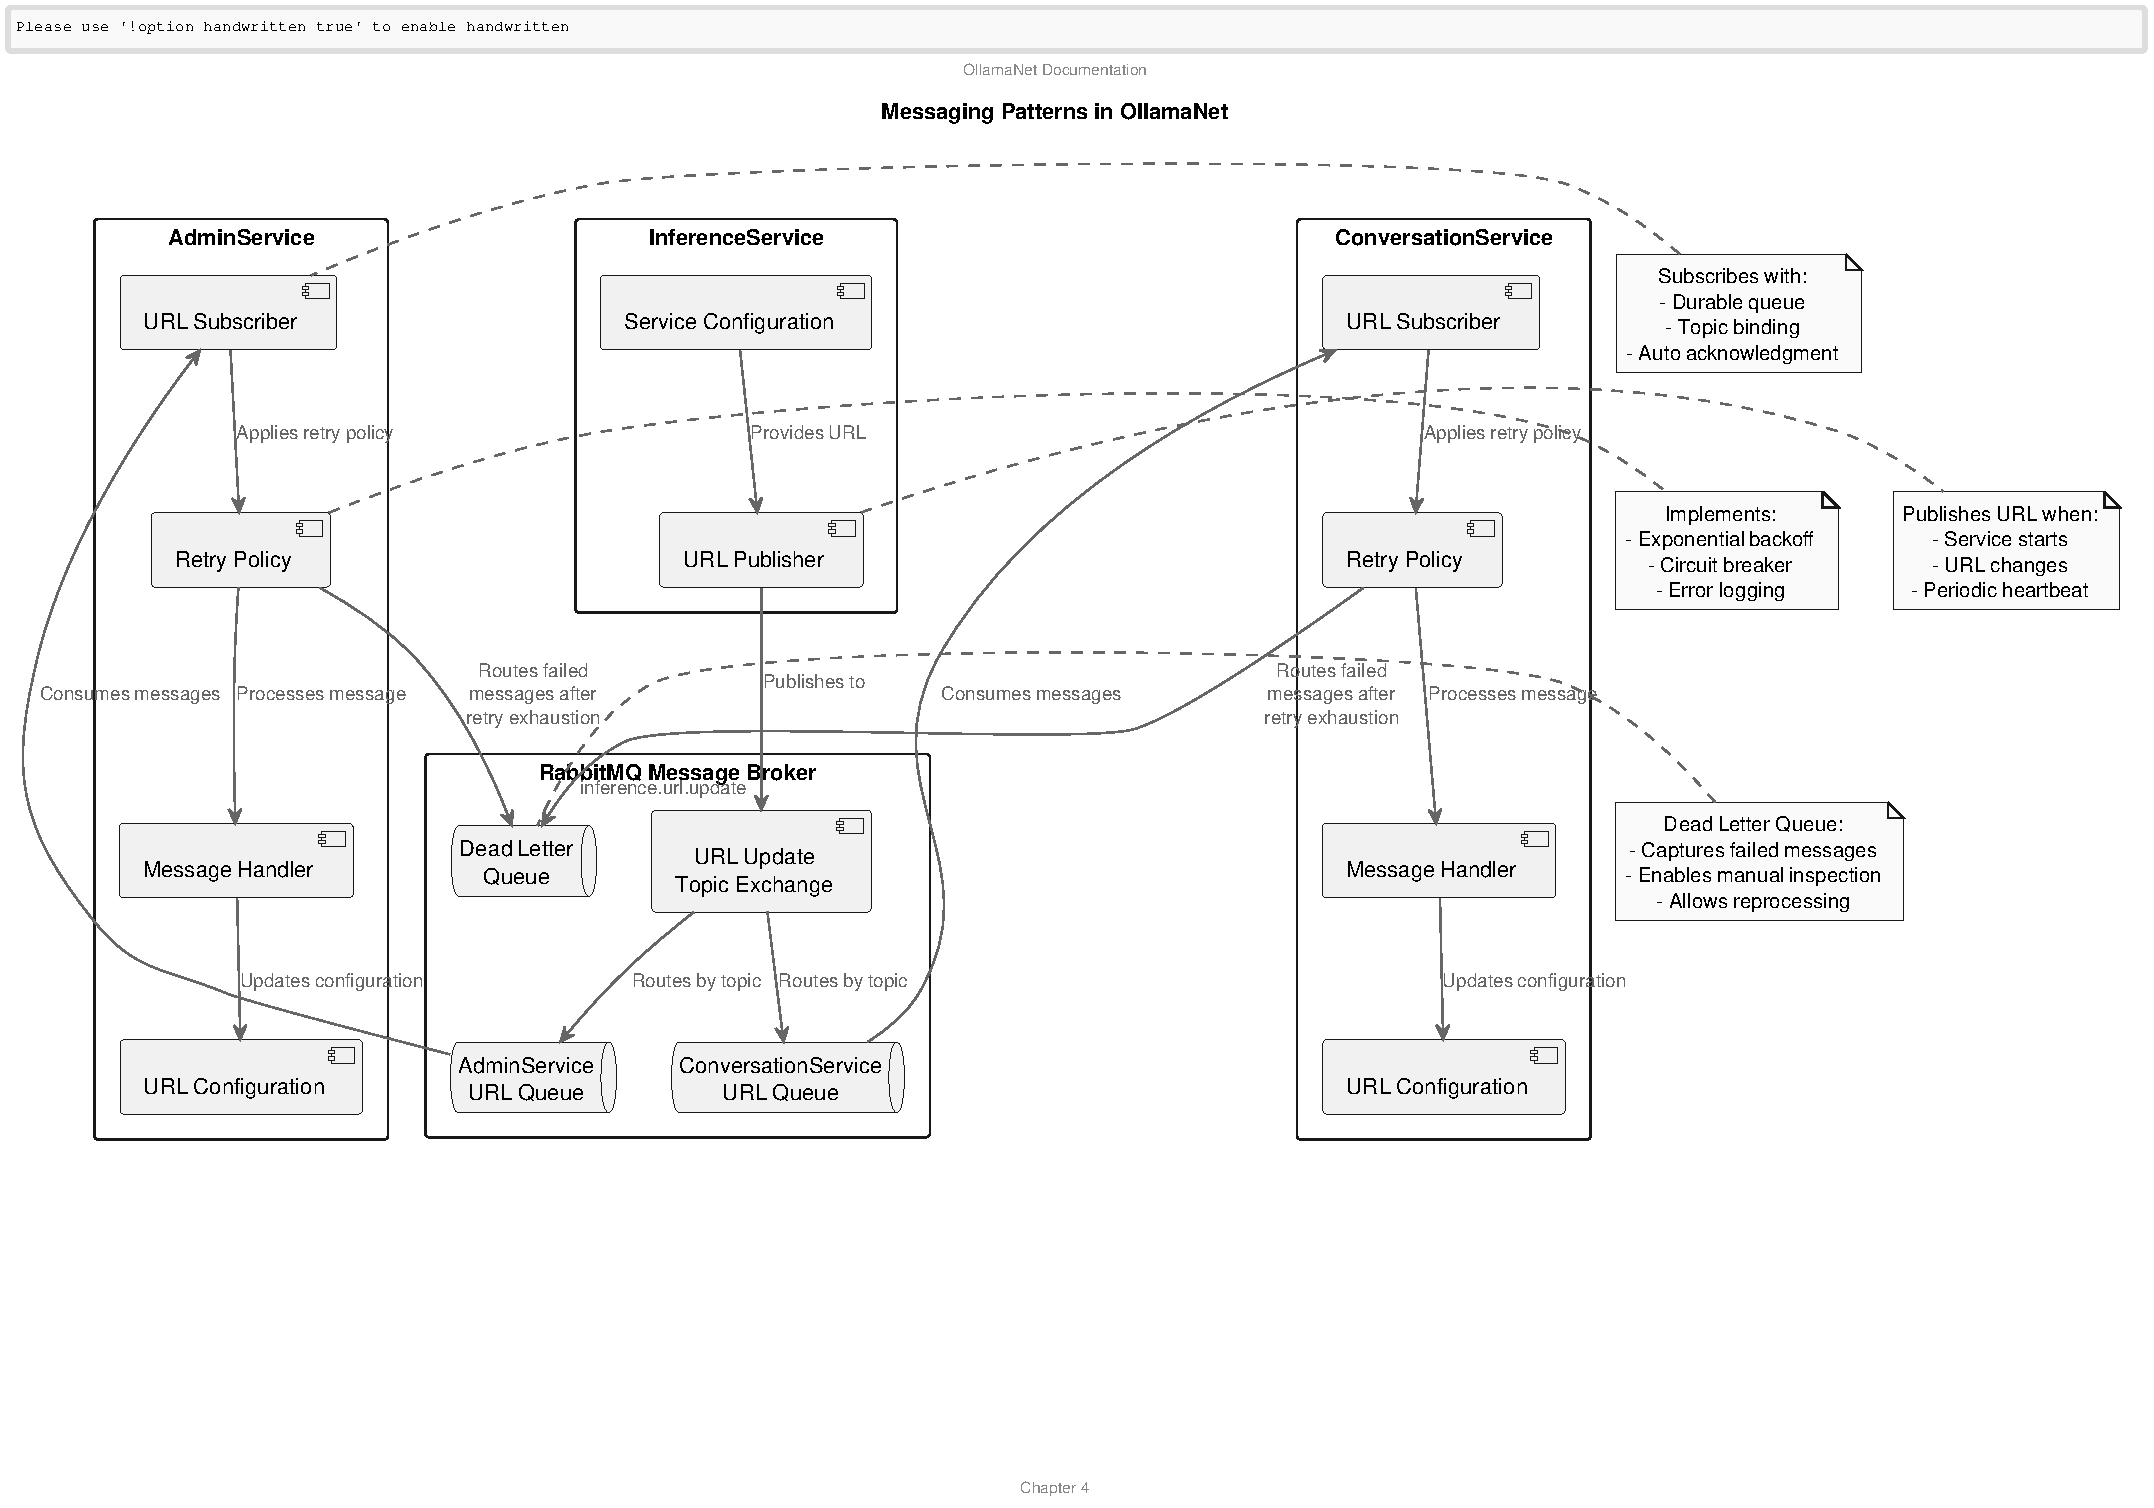
\includegraphics[width=\textwidth]{./Chapter04/figures/messaging_patterns.pdf}
    \caption{Message Broker Communication Patterns}
    \label{fig:messaging-patterns}
\end{sidewaysfigure}
\clearpage

\subsubsection{Event-Driven Communication}

The system uses event-driven communication for:

\begin{enumerate}
   \item \textbf{Service Discovery}: Inference Service publishes URL updates.
   \item \textbf{State Changes}: Services publish events when important state changes occur.
   \item \textbf{Asynchronous Processing}: Long-running operations use events for completion notification.
   \item \textbf{Integration Events}: Cross-service business processes use events for coordination.
\end{enumerate}

\subsubsection{Message Formats and Standards}

Messages follow these standards:

\begin{enumerate}
   \item \textbf{JSON Format}: All messages use JSON for compatibility.
   \item \textbf{Metadata Inclusion}: Messages include metadata like timestamp and version.
   \item \textbf{Schema Validation}: Messages are validated against schemas.
   \item \textbf{Versioning}: Message formats include version information for compatibility.
\end{enumerate}

\begin{verbatim}
{
  "newUrl": "https://example-inference-engine.ngrok-free.app/",
  "timestamp": "2023-08-15T14:30:00Z",
  "serviceId": "inference-engine",
  "version": "1.0"
}
\end{verbatim}

\subsubsection{Publishing and Subscribing Mechanisms}

The system implements these messaging patterns:

\begin{enumerate}
   \item \textbf{Publish-Subscribe}: One publisher, multiple subscribers.
   \item \textbf{Work Queues}: Tasks distributed among multiple workers.
   \item \textbf{RPC}: Request-reply pattern over messaging.
   \item \textbf{Broadcast}: Messages sent to all interested parties.
\end{enumerate}

\begin{verbatim}
public async Task PublishInferenceUrlUpdate(string newUrl)
{
    var message = new InferenceUrlUpdateMessage
    {
        NewUrl = newUrl,
        Timestamp = DateTime.UtcNow
    };
    
    var factory = new ConnectionFactory
    {
        HostName = _options.HostName,
        Port = _options.Port,
        UserName = _options.UserName,
        Password = _options.Password,
        VirtualHost = _options.VirtualHost
    };
    
    using var connection = factory.CreateConnection();
    using var channel = connection.CreateModel();
    
    channel.ExchangeDeclare(
        exchange: _options.Exchange,
        type: ExchangeType.Topic,
        durable: true);
        
    var json = JsonSerializer.Serialize(message);
    var body = Encoding.UTF8.GetBytes(json);
    
    channel.BasicPublish(
        exchange: _options.Exchange,
        routingKey: _options.InferenceUrlRoutingKey,
        basicProperties: null,
        body: body);
}
\end{verbatim}

\section{Cross-Cutting Concerns}

\subsection{Authentication \& Authorization}

\subsubsection{JWT Implementation}

OllamaNet implements JWT-based authentication:

\begin{enumerate}
   \item \textbf{Token Issuance}: The Auth Service issues JWT tokens upon successful login.
   \item \textbf{Token Validation}: The Gateway and services validate tokens before processing requests.
   \item \textbf{Claims-Based Identity}: Tokens contain claims about the user's identity and roles.
   \item \textbf{Refresh Tokens}: Long-lived refresh tokens enable session persistence.
\end{enumerate}

\subsubsection{Role-Based Access Control}

The system implements role-based access control:

\begin{enumerate}
   \item \textbf{Role Definitions}: Users are assigned roles (Admin, User, etc.).
   \item \textbf{Permission Mapping}: Roles map to permissions for specific operations.
   \item \textbf{Gateway Enforcement}: The Gateway enforces role requirements for routes.
   \item \textbf{Service-Level Checks}: Services perform additional authorization checks as needed.
\end{enumerate}

\begin{verbatim}
{
  "RoleAuthorization": [
    {
      "PathTemplate": "/api/admin/*",
      "RequiredRole": "Admin"
    },
    {
      "PathTemplate": "/api/conversations/*",
      "RequiredRole": "User"
    }
  ]
}
\end{verbatim}

\subsubsection{Claims Forwarding Between Services}

User claims are forwarded between services:

\begin{enumerate}
   \item \textbf{Gateway Extraction}: The Gateway extracts claims from JWT tokens.
   \item \textbf{Header Injection}: Claims are added as HTTP headers to downstream requests.
   \item \textbf{Service Validation}: Services validate and use the forwarded claims.
   \item \textbf{Consistent Identity}: User identity is maintained across service boundaries.
\end{enumerate}

\subsection{Logging \& Monitoring}

\subsubsection{Centralized Logging Approach}

OllamaNet implements centralized logging:

\begin{enumerate}
   \item \textbf{Structured Logging}: All logs use a structured format (JSON).
   \item \textbf{Log Levels}: Appropriate log levels (Debug, Info, Warning, Error) are used.
   \item \textbf{Correlation IDs}: Requests are tracked across services using correlation IDs.
   \item \textbf{Contextual Information}: Logs include relevant context for troubleshooting.
\end{enumerate}

\subsubsection{Monitoring Strategies}

The system is monitored through:

\begin{enumerate}
   \item \textbf{Health Checks}: Services expose health check endpoints.
   \item \textbf{Metrics Collection}: Key performance metrics are collected.
   \item \textbf{Alerting}: Alerts are triggered for critical issues.
   \item \textbf{Dashboard Visualization}: Metrics are visualized in dashboards.
\end{enumerate}

\subsubsection{Observability Features}

Observability is achieved through:

\begin{enumerate}
   \item \textbf{Distributed Tracing}: Requests are traced across service boundaries.
   \item \textbf{Performance Metrics}: Response times, throughput, and error rates are tracked.
   \item \textbf{Resource Utilization}: CPU, memory, and network usage are monitored.
   \item \textbf{Business Metrics}: Key business metrics are tracked for insights.
\end{enumerate}

\subsection{Resilience Patterns}

\subsubsection{Circuit Breaker Patterns}

Circuit breakers prevent cascading failures:

\begin{enumerate}
   \item \textbf{Failure Detection}: Tracks failures in downstream service calls.
   \item \textbf{Open Circuit}: Stops calls to failing services after threshold is reached.
   \item \textbf{Half-Open State}: Allows test calls to check if service has recovered.
   \item \textbf{Closed Circuit}: Normal operation when service is healthy.
\end{enumerate}

\begin{verbatim}
// Configure HTTP client with circuit breaker
services.AddHttpClient<IInferenceEngineConnector, InferenceEngineConnector>()
    .AddPolicyHandler(GetCircuitBreakerPolicy());
    
private IAsyncPolicy<HttpResponseMessage> GetCircuitBreakerPolicy()
{
    return HttpPolicyExtensions
        .HandleTransientHttpError()
        .CircuitBreakerAsync(
            handledEventsAllowedBeforeBreaking: 5,
            durationOfBreak: TimeSpan.FromSeconds(30)
        );
}
\end{verbatim}

\subsubsection{Retry Policies}

Retry policies handle transient failures:

\begin{enumerate}
   \item \textbf{Retry Count}: Specifies how many retries to attempt.
   \item \textbf{Backoff Strategy}: Implements exponential backoff between retries.
   \item \textbf{Retry Triggers}: Defines which errors trigger retries.
   \item \textbf{Timeout}: Sets maximum time for operation with retries.
\end{enumerate}

\begin{verbatim}
private IAsyncPolicy<HttpResponseMessage> GetRetryPolicy()
{
    return HttpPolicyExtensions
        .HandleTransientHttpError()
        .OrResult(msg => msg.StatusCode == System.Net.HttpStatusCode.TooManyRequests)
        .WaitAndRetryAsync(
            retryCount: 3,
            sleepDurationProvider: retryAttempt => TimeSpan.FromSeconds(Math.Pow(2, retryAttempt))
        );
}
\end{verbatim}

\subsubsection{Timeout Management}

The system manages timeouts at multiple levels:

\begin{enumerate}
   \item \textbf{Request Timeouts}: HTTP requests have appropriate timeouts.
   \item \textbf{Operation Timeouts}: Complex operations have overall timeouts.
   \item \textbf{Graceful Degradation}: Services degrade gracefully when timeouts occur.
   \item \textbf{User Feedback}: Users are informed about timeouts when appropriate.
\end{enumerate}

\subsubsection{Fallback Strategies}

Fallback strategies provide alternatives when operations fail:

\begin{enumerate}
   \item \textbf{Cached Data}: Return cached data when live data is unavailable.
   \item \textbf{Default Values}: Use sensible defaults when actual values cannot be retrieved.
   \item \textbf{Degraded Functionality}: Provide limited functionality rather than complete failure.
   \item \textbf{User Notification}: Inform users when fallbacks are used.
\end{enumerate}

\begin{terminology}
\begin{description}
    \item[API Gateway] Component that acts as an entry point for client requests to microservices
    \item[Circuit Breaker] Pattern that prevents cascading failures across services
    \item[JWT] JSON Web Token used for authentication between services
    \item[Microservice] Independent deployable service with a specific domain responsibility
    \item[RabbitMQ] Message broker used for asynchronous communication and service discovery
\end{description}
\end{terminology}
\cleardoublepage
\def\chapdir{./Chapter05}

\chapter{Database Layer} \label{ch:database-layer}

\section{Database Architecture}

\subsection{Overall Database Design Philosophy}

The OllamaNet platform employs a robust database architecture that balances the needs of a microservices ecosystem with the benefits of relational data integrity. The database layer is designed around several key principles:

\begin{enumerate}
   \item \textbf{Shared Database with Logical Separation}: While microservices often employ separate databases, OllamaNet uses a shared SQL Server database with logical separation to maintain data integrity while providing service isolation.

   \item \textbf{Repository Pattern}: Data access is abstracted through repositories, providing a consistent interface for services to interact with the database.

   \item \textbf{Unit of Work Pattern}: Transactions across multiple repositories are coordinated through a Unit of Work implementation, ensuring data consistency.

   \item \textbf{Domain-Driven Design}: The database schema reflects the domain model, with clear entity boundaries and relationships that map to business concepts.

   \item \textbf{Soft Delete}: Entities implement soft deletion to preserve historical data while allowing logical removal.
\end{enumerate}

\begin{figure}
    \centering
    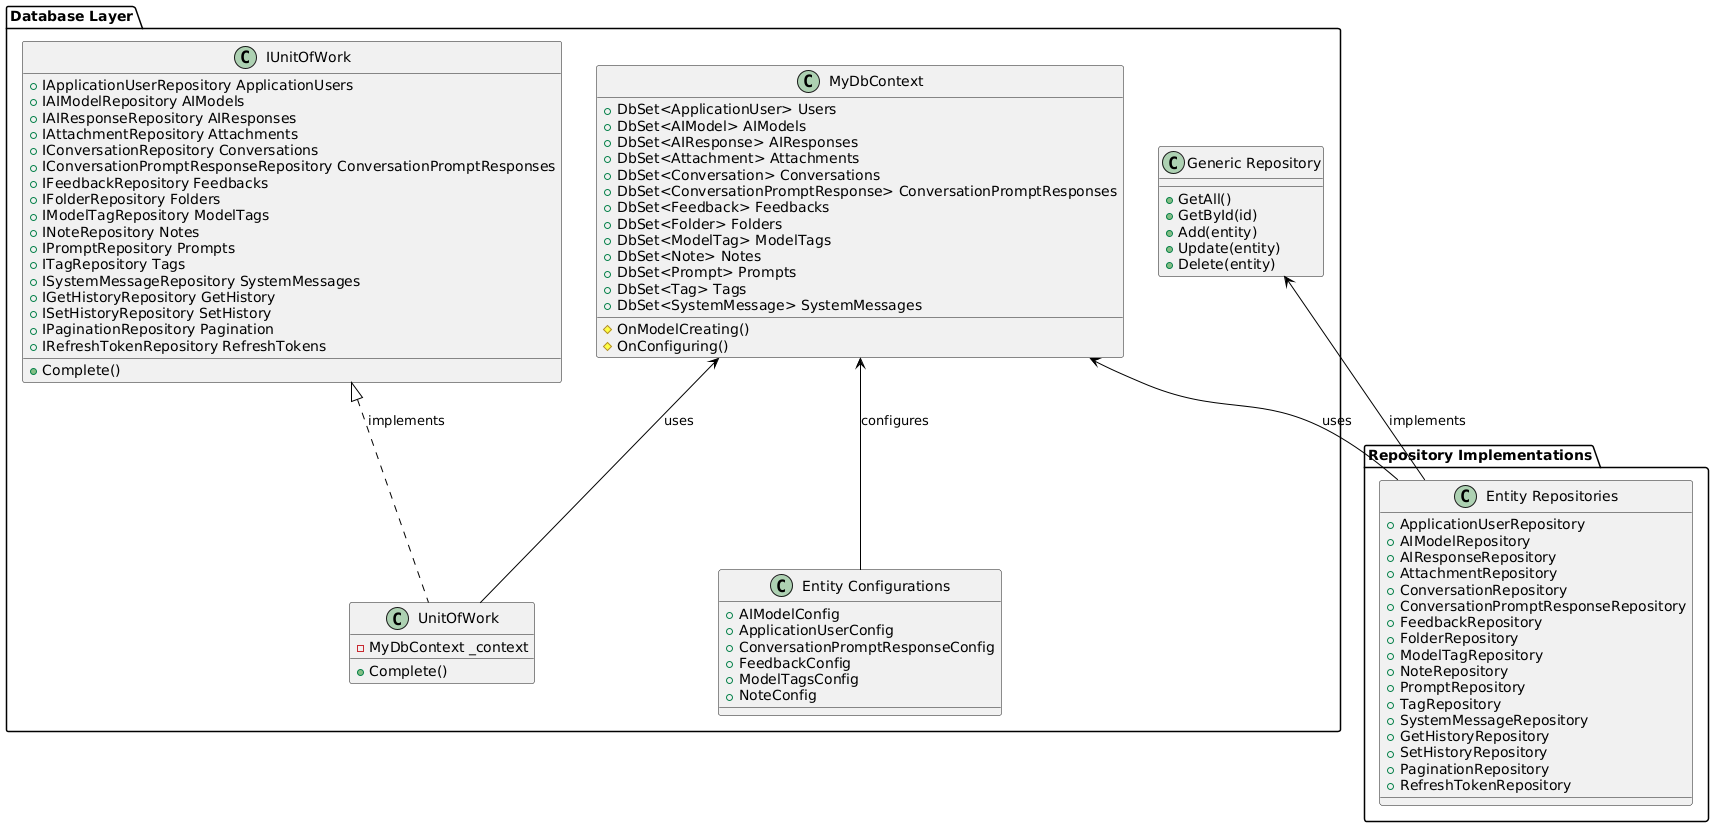
\includegraphics[width=0.8\textwidth]{./Chapter05/figures/database_architecture.png}
    \caption{Database Architecture Overview}
    \label{fig:database-architecture}
\end{figure}

\subsection{Database Per Service Pattern Consideration}

The OllamaNet architecture considered the Database-per-Service pattern, which is common in microservices architectures, but ultimately chose a shared database approach for several reasons:

\begin{enumerate}
   \item \textbf{Data Integrity}: A shared database ensures referential integrity across services, which is particularly important for user data and relationships.

   \item \textbf{Simplified Deployment}: A single database reduces operational complexity compared to managing multiple databases.

   \item \textbf{Query Efficiency}: Cross-service queries can be performed more efficiently within a single database.

   \item \textbf{Transaction Support}: ACID transactions across related data are easier to implement in a shared database.
\end{enumerate}

However, to maintain service independence, the architecture implements logical separation through:

\begin{enumerate}
   \item \textbf{Service-Specific Repositories}: Each service accesses only its relevant entities through dedicated repositories.

   \item \textbf{Schema Namespacing}: Database tables are organized into logical groups aligned with service boundaries.

   \item \textbf{Access Control}: Services are restricted to their own data domains through repository interfaces.
\end{enumerate}

\subsection{Shared Database Implementation}

The shared database implementation uses Entity Framework Core as an ORM, with the following components:

\begin{enumerate}
   \item \textbf{Central DbContext}: A single \texttt{MyDbContext} class that extends \texttt{IdentityDbContext<ApplicationUser>} and includes all entity DbSets.

   \item \textbf{Entity Configuration}: Entity relationships and constraints are configured in the \texttt{OnModelCreating} method of the DbContext.

   \item \textbf{Service-Specific Repositories}: Each service has dedicated repositories that access only the entities relevant to that service.

   \item \textbf{Unit of Work Coordinator}: A central \texttt{UnitOfWork} class coordinates operations across repositories and manages transactions.
\end{enumerate}

\begin{verbatim}
public class MyDbContext : IdentityDbContext<ApplicationUser>
{
    public MyDbContext(DbContextOptions<MyDbContext> options) : base(options) { }

    public DbSet<AIModel> AIModels { get; set; }
    public DbSet<AIResponse> AIResponses { get; set; }
    public DbSet<Attachment> Attachments { get; set; }
    public DbSet<Conversation> Conversations { get; set; }
    public DbSet<ConversationPromptResponse> ConversationPromptResponses { get; set; }
    public DbSet<Feedback> Feedbacks { get; set; }
    public DbSet<ModelTag> ModelTags { get; set; }
    public DbSet<Prompt> Prompts { get; set; }
    public DbSet<RefreshToken> RefreshTokens { get; set; }
    public DbSet<SystemMessage> SystemMessages { get; set; }
    public DbSet<Tag> Tags { get; set; }

    protected override void OnModelCreating(ModelBuilder modelBuilder)
    {
        base.OnModelCreating(modelBuilder);

        // Configure ModelTag as a join entity
        modelBuilder.Entity<ModelTag>().HasKey(mt => new { mt.ModelId, mt.TagId });

        // Other entity configurations...
    }
}
\end{verbatim}

\subsection{Physical vs. Logical Database Separation}

OllamaNet employs logical separation within a physically shared database:

\begin{enumerate}
   \item \textbf{Physical Sharing}: All services access the same SQL Server instance and database.

   \item \textbf{Logical Separation}:
   \begin{itemize}
      \item Each service accesses only its domain-specific entities
      \item Repository interfaces expose only relevant operations
      \item Service boundaries are enforced at the application level
   \end{itemize}
\end{enumerate}

This approach provides several benefits:

\begin{itemize}
   \item \textbf{Data Consistency}: Ensures consistent data across services.
   \item \textbf{Simplified Transactions}: Enables ACID transactions across related entities.
   \item \textbf{Efficient Queries}: Allows for efficient joins between related entities.
   \item \textbf{Reduced Operational Complexity}: Simplifies database management and deployment.
\end{itemize}

\begin{figure}
    \centering
    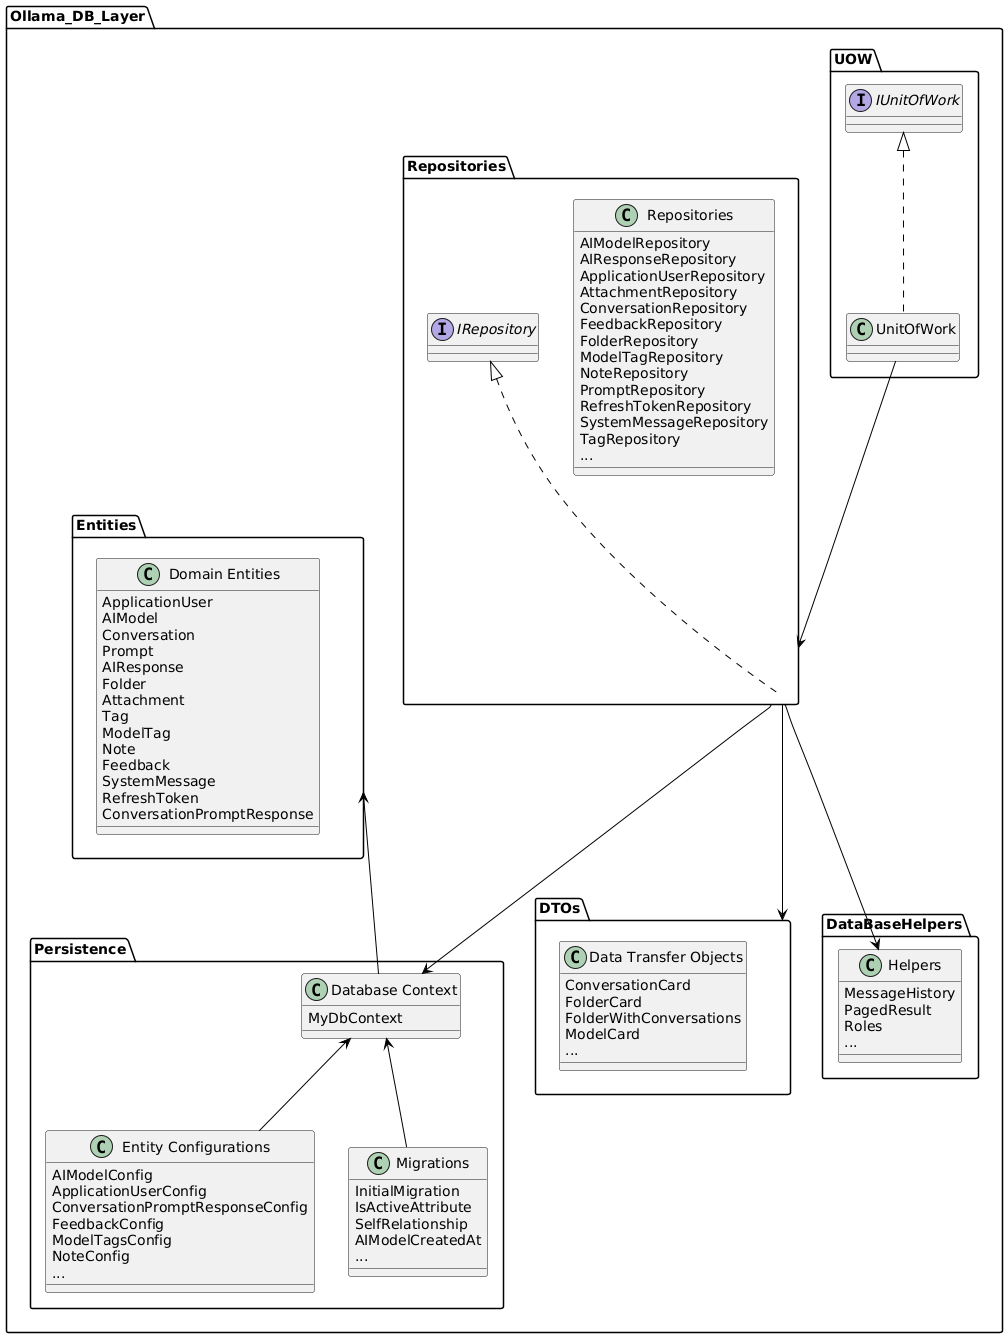
\includegraphics[width=0.8\textwidth]{./Chapter05/figures/logical_separation.png}
    \caption{Physical vs Logical Database Separation}
    \label{fig:logical-separation}
\end{figure}

\subsection{Design Principles and Patterns}

The database layer implements several key design principles and patterns:

\subsubsection*{Repository Pattern}

Abstracts data access logic and provides a consistent interface for working with entities.

\begin{verbatim}
public interface IRepository<T> where T : class
{
    Task<IEnumerable<T>> GetAllAsync();
    Task<T> GetByIdAsync(string id);
    Task<bool> AddAsync(T entity);
    Task<bool> UpdateAsync(T entity);
    Task<bool> DeleteAsync(string id);
    Task<bool> SoftDeleteAsync(string id);
    Task<bool> ExistsAsync(string id);
}
\end{verbatim}

\subsubsection*{Unit of Work Pattern}

Coordinates operations across multiple repositories and provides a single point for committing changes.

\begin{verbatim}
public interface IUnitOfWork : IDisposable
{
    IAIModelRepository AIModels { get; }
    IAIResponseRepository AIResponses { get; }
    // Other repositories...
    
    Task<int> SaveChangesAsync();
}
\end{verbatim}

\subsubsection*{Identity Integration}

Extends ASP.NET Identity with custom user properties and relationships.

\subsubsection*{Soft Delete Pattern}

Implements logical deletion through an \texttt{IsDeleted} flag on entities.

\subsubsection*{Query Specification Pattern}

Encapsulates query logic for complex filtering and sorting.

\subsubsection*{Eager Loading Strategy}

Uses explicit loading of related entities to avoid N+1 query problems.

\section{Data Models}

\subsection{Entity Relationship Diagrams}

The OllamaNet database schema includes several interconnected entities that support the platform's functionality:

\begin{figure}
    \centering
    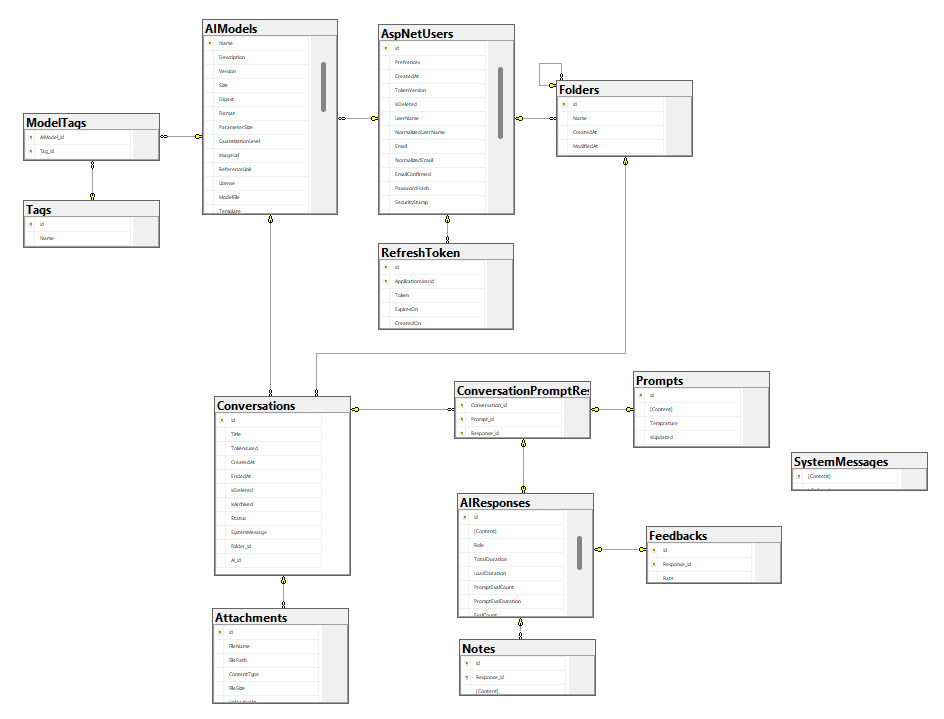
\includegraphics[width=0.8\textwidth]{./Chapter05/figures/entity_relationship.png}
    \caption{Entity Relationship Diagram}
    \label{fig:entity-relationship}
\end{figure}

\subsection{Schema Designs}

The database schema is organized around several key domains:

\begin{enumerate}
   \item \textbf{User Management Domain}:
   \begin{itemize}
      \item ApplicationUser (extends IdentityUser)
      \item RefreshToken
   \end{itemize}

   \item \textbf{Model Management Domain}:
   \begin{itemize}
      \item AIModel
      \item Tag
      \item ModelTag (junction entity)
   \end{itemize}

   \item \textbf{Conversation Domain}:
   \begin{itemize}
      \item Conversation
      \item ConversationPromptResponse
      \item Prompt
      \item AIResponse
      \item Attachment
      \item Feedback
   \end{itemize}

   \item \textbf{System Configuration Domain}:
   \begin{itemize}
      \item SystemMessage
   \end{itemize}
\end{enumerate}

Each entity includes standard fields for tracking creation, modification, and deletion:

\begin{verbatim}
// Common fields found in most entities
public string Id { get; set; }
public DateTime CreatedAt { get; set; }
public bool IsDeleted { get; set; }
\end{verbatim}

\subsection{Domain Model to Database Mapping}

The OllamaNet platform maps its domain model to the database schema using Entity Framework Core's fluent API and data annotations:

\begin{enumerate}
   \item \textbf{Entity Configuration}:
   \begin{itemize}
      \item Primary keys defined using the \texttt{[Key]} attribute or fluent API
      \item Foreign keys established through the fluent API
      \item Navigation properties configured for relationships
   \end{itemize}

   \item \textbf{Relationship Mapping}:
   \begin{itemize}
      \item One-to-Many: Defined through navigation properties and foreign keys
      \item Many-to-Many: Implemented using junction entities (e.g., ModelTag)
      \item One-to-One: Configured with unique foreign keys
   \end{itemize}

   \item \textbf{Property Mapping}:
   \begin{itemize}
      \item Data types specified through attributes or fluent API
      \item Required fields marked with the \texttt{[Required]} attribute
      \item String length constraints applied where appropriate
   \end{itemize}
\end{enumerate}

Example of entity configuration in the DbContext:

\begin{verbatim}
protected override void OnModelCreating(ModelBuilder modelBuilder)
{
    base.OnModelCreating(modelBuilder);

    // Configure ModelTag as a join entity
    modelBuilder.Entity<ModelTag>().HasKey(mt => new { mt.ModelId, mt.TagId });

    modelBuilder.Entity<ModelTag>()
        .HasOne(mt => mt.Model)
        .WithMany(m => m.ModelTags)
        .HasForeignKey(mt => mt.ModelId);

    modelBuilder.Entity<ModelTag>()
        .HasOne(mt => mt.Tag)
        .WithMany(t => t.ModelTags)
        .HasForeignKey(mt => mt.TagId);
}
\end{verbatim}

\subsection{Database Constraints and Validations}

The OllamaNet database implements several types of constraints and validations:

\begin{enumerate}
   \item \textbf{Primary Key Constraints}: Each entity has a unique identifier, typically a string containing a GUID.

   \item \textbf{Foreign Key Constraints}: Relationships between entities are enforced through foreign keys.

   \item \textbf{Required Field Constraints}: Critical fields are marked as required to prevent null values.

   \item \textbf{String Length Constraints}: String fields have appropriate length constraints.

   \item \textbf{Unique Constraints}: Applied to fields that must be unique, such as usernames and email addresses.

   \item \textbf{Default Values}: Some fields have default values, such as \texttt{IsDeleted = false} and \texttt{CreatedAt = DateTime.UtcNow}.

   \item \textbf{Check Constraints}: Used to enforce business rules, such as valid status values.
\end{enumerate}

These constraints are implemented through a combination of Entity Framework Core configurations and database-level constraints.

\subsection{Soft Delete Implementation}

OllamaNet implements soft deletion across its entities to preserve historical data while allowing logical removal:

\begin{enumerate}
   \item \textbf{IsDeleted Flag}: Each entity includes an \texttt{IsDeleted} boolean property.

   \item \textbf{Repository Filtering}: Repositories automatically filter out entities where \texttt{IsDeleted = true}.

\begin{verbatim}
public async Task<IEnumerable<Tag>> GetAllAsync()
{
    return await _context.Tags
        .Where(t => !t.IsDeleted)
        .ToListAsync();
}
\end{verbatim}

   \item \textbf{Soft Delete Operation}: Instead of physically removing entities, the \texttt{SoftDeleteAsync} method sets \texttt{IsDeleted = true}.

\begin{verbatim}
public async Task<bool> SoftDeleteAsync(string id)
{
    var tag = await _context.Tags.FindAsync(id);
    if (tag == null)
        return false;

    tag.IsDeleted = true;
    _context.Tags.Update(tag);
    return true;
}
\end{verbatim}

   \item \textbf{Query Extensions}: Extension methods automatically apply soft delete filtering to queries.
\end{enumerate}

This approach provides several benefits:
\begin{itemize}
   \item Preserves historical data for auditing and analysis
   \item Allows for data recovery if needed
   \item Maintains referential integrity across related entities
   \item Simplifies compliance with data retention requirements
\end{itemize}

\section{Data Consistency Strategies}

\subsection{Eventual Consistency Approaches}

While OllamaNet primarily uses a shared database with strong consistency, it also implements eventual consistency patterns for specific scenarios:

\begin{enumerate}
   \item \textbf{Cache Synchronization}: Redis caching is used with appropriate invalidation strategies to ensure eventual consistency between the cache and the database.

   \item \textbf{Read-Your-Writes Consistency}: The system ensures that after a write operation, subsequent reads will reflect the changes, even when caching is involved.

   \item \textbf{Background Processing}: Some operations are performed asynchronously, with eventual consistency guaranteed through reliable message processing.

   \item \textbf{Optimistic Concurrency}: Entity Framework's optimistic concurrency control is used to detect and resolve conflicts when multiple services update the same data.
\end{enumerate}

\subsection{Saga Pattern Implementation}

For complex operations that span multiple services, OllamaNet implements a simplified version of the Saga pattern:

\begin{enumerate}
   \item \textbf{Coordinated Transactions}: The Unit of Work pattern coordinates transactions within a single service.

   \item \textbf{Compensating Transactions}: For cross-service operations, compensating transactions are implemented to roll back changes if a step fails.

   \item \textbf{Event-Driven Coordination}: Services publish events to signal completion of their part of a distributed transaction.
\end{enumerate}

This approach helps maintain data consistency across service boundaries while avoiding distributed transactions.

\subsection{Distributed Transactions Handling}

OllamaNet avoids distributed transactions where possible, but implements several strategies for maintaining consistency across services:

\begin{enumerate}
   \item \textbf{Service Composition}: Complex operations are composed at the API level rather than using distributed transactions.

   \item \textbf{Event-Driven Updates}: Services subscribe to events from other services to update their data accordingly.

   \item \textbf{Idempotent Operations}: APIs are designed to be idempotent, allowing safe retries of failed operations.

   \item \textbf{Consistency Verification}: Background processes verify and reconcile data consistency across services.
\end{enumerate}

\subsection{Concurrency Control Mechanisms}

The database layer implements several concurrency control mechanisms:

\begin{enumerate}
   \item \textbf{Optimistic Concurrency}: Entity Framework's optimistic concurrency control is used to detect conflicts during updates.

\begin{verbatim}
modelBuilder.Entity<AIModel>()
    .Property(p => p.RowVersion)
    .IsRowVersion();
\end{verbatim}

   \item \textbf{Pessimistic Locking}: For critical operations, explicit database locks are used to prevent concurrent modifications.

   \item \textbf{Transaction Isolation Levels}: Appropriate transaction isolation levels are set based on the operation's requirements.

\begin{verbatim}
using var transaction = await _context.Database.BeginTransactionAsync(IsolationLevel.ReadCommitted);
try
{
    // Perform operations
    await _context.SaveChangesAsync();
    await transaction.CommitAsync();
}
catch
{
    await transaction.RollbackAsync();
    throw;
}
\end{verbatim}
\end{enumerate}

\subsection{Error Handling and Rollback Strategies}

The database layer implements robust error handling and rollback strategies:

\begin{enumerate}
   \item \textbf{Transaction Scope}: Operations that modify multiple entities are wrapped in transactions to ensure atomicity.

\begin{verbatim}
public async Task<bool> CreateConversationWithPromptAsync(Conversation conversation, Prompt prompt, AIResponse response)
{
    // Add entities
    await _unitOfWork.Conversations.AddAsync(conversation);
    await _unitOfWork.Prompts.AddAsync(prompt);
    await _unitOfWork.AIResponses.AddAsync(response);
    
    // Create relationship
    var cpr = new ConversationPromptResponse
    {
        Id = Guid.NewGuid().ToString(),
        ConversationId = conversation.Id,
        PromptId = prompt.Id,
        AIResponseId = response.Id,
        CreatedAt = DateTime.UtcNow
    };
    
    await _unitOfWork.ConversationPromptResponses.AddAsync(cpr);
    
    // Save all changes in a single transaction
    await _unitOfWork.SaveChangesAsync();
    
    return true;
}
\end{verbatim}

   \item \textbf{Exception Handling}: Exceptions during database operations are caught and handled appropriately, with transactions rolled back when necessary.

   \item \textbf{Retry Logic}: Transient errors are handled with retry logic to improve resilience.

   \item \textbf{Logging}: Database errors are logged with sufficient context for troubleshooting.
\end{enumerate}

\section{Database Technologies}

\subsection{SQL Server Implementation Details}

OllamaNet uses SQL Server as its primary database technology:

\begin{enumerate}
   \item \textbf{Version}: SQL Server 2019 or later, supporting modern features like JSON support and improved performance.

   \item \textbf{Connection Management}: Connection pooling is configured for optimal performance and resource utilization.

   \item \textbf{Indexing Strategy}: Appropriate indexes are created for frequently queried fields to optimize performance.

   \item \textbf{Query Optimization}: Complex queries are optimized using query hints and execution plan analysis.

   \item \textbf{Security Configuration}: SQL Server is configured with appropriate security settings, including encryption and access controls.
\end{enumerate}

\subsection{Entity Framework Core Configuration}

Entity Framework Core is configured for optimal performance and functionality:

\begin{enumerate}
   \item \textbf{DbContext Configuration}: The \texttt{MyDbContext} is configured with appropriate options for tracking, batching, and logging.

\begin{verbatim}
services.AddDbContext<MyDbContext>(options =>
    options.UseSqlServer(Configuration.GetConnectionString("DefaultConnection"),
        sqlOptions =>
        {
            sqlOptions.EnableRetryOnFailure(
                maxRetryCount: 5,
                maxRetryDelay: TimeSpan.FromSeconds(30),
                errorNumbersToAdd: null);
        })
    .UseQueryTrackingBehavior(QueryTrackingBehavior.NoTracking)
    .EnableSensitiveDataLogging(isDevelopment));
\end{verbatim}

   \item \textbf{Entity Configuration}: Entities are configured using a combination of data annotations and the fluent API.

   \item \textbf{Lazy Loading}: Lazy loading is disabled by default to prevent N+1 query problems, with explicit loading used when needed.

   \item \textbf{Query Filters}: Global query filters are applied for soft delete and multi-tenancy.

\begin{verbatim}
modelBuilder.Entity<Conversation>()
    .HasQueryFilter(c => !c.IsDeleted);
\end{verbatim}

   \item \textbf{Performance Optimization}: Query compilation is cached, and query execution is optimized through appropriate includes and projections.
\end{enumerate}

\subsection{Redis Caching Implementation}

OllamaNet uses Redis for distributed caching to improve performance:

\begin{enumerate}
   \item \textbf{Cache Architecture}: A multi-level caching approach with in-memory and Redis caches.

   \item \textbf{Cache-Aside Pattern}: Data is retrieved from the cache first, with database fallback when needed.

\begin{verbatim}
public async Task<T> GetOrSetAsync<T>(string key, Func<Task<T>> factory, TimeSpan? expiry = null)
{
    try
    {
        var cachedValue = await _redisCacheService.GetAsync<T>(key);
        if (cachedValue != null)
        {
            _logger.LogDebug("Cache hit for key: {Key}", key);
            return cachedValue;
        }

        _logger.LogDebug("Cache miss for key: {Key}", key);
        var result = await factory();
        
        if (result != null)
        {
            await _redisCacheService.SetAsync(key, result, expiry ?? _defaultExpiry);
        }
        
        return result;
    }
    catch (Exception ex)
    {
        _logger.LogWarning(ex, "Cache operation failed for key: {Key}, falling back to data source", key);
        return await factory();
    }
}
\end{verbatim}

   \item \textbf{Cache Invalidation}: When data changes, related cache entries are invalidated to maintain consistency.

   \item \textbf{Cache Resilience}: The system gracefully handles Redis unavailability by falling back to the database.

   \item \textbf{Cache Optimization}: Frequently accessed data is cached with appropriate expiration policies.
\end{enumerate}

\subsection{Query Optimization Techniques}

OllamaNet implements several query optimization techniques:

\begin{enumerate}
   \item \textbf{Indexing Strategy}: Appropriate indexes are created for frequently queried fields.

   \item \textbf{Query Projection}: Queries project only the required fields rather than loading entire entities.

\begin{verbatim}
public async Task<IEnumerable<ModelDto>> GetAllModelsAsync()
{
    return await _context.AIModels
        .Where(m => !m.IsDeleted)
        .Select(m => new ModelDto
        {
            Id = m.Id,
            Name = m.Name,
            Description = m.Description,
            // Only select needed properties
        })
        .ToListAsync();
}
\end{verbatim}

   \item \textbf{Eager Loading}: Related entities are loaded using explicit includes to avoid N+1 query problems.

\begin{verbatim}
public async Task<Conversation> GetConversationWithDetailsAsync(string id)
{
    return await _context.Conversations
        .Include(c => c.ConversationPromptResponses)
            .ThenInclude(cpr => cpr.Prompt)
        .Include(c => c.ConversationPromptResponses)
            .ThenInclude(cpr => cpr.AIResponse)
        .FirstOrDefaultAsync(c => c.Id == id && !c.IsDeleted);
}
\end{verbatim}

   \item \textbf{Pagination}: Large result sets are paginated to improve performance.

\begin{verbatim}
public async Task<IEnumerable<Conversation>> GetConversationsPagedAsync(
    string userId, int pageNumber, int pageSize)
{
    return await _context.Conversations
        .Where(c => c.UserId == userId && !c.IsDeleted)
        .OrderByDescending(c => c.CreatedAt)
        .Skip((pageNumber - 1) * pageSize)
        .Take(pageSize)
        .ToListAsync();
}
\end{verbatim}

   \item \textbf{Query Caching}: Frequently executed queries are cached to reduce database load.
\end{enumerate}

\subsection{Connection Management}

OllamaNet implements effective connection management strategies:

\begin{enumerate}
   \item \textbf{Connection Pooling}: Entity Framework Core's connection pooling is configured for optimal performance.

   \item \textbf{Connection Resilience}: Retry logic is implemented for transient connection failures.

   \item \textbf{Connection Monitoring}: Connection usage is monitored to detect leaks and performance issues.

   \item \textbf{Connection Timeout}: Appropriate connection timeouts are configured to prevent resource exhaustion.

   \item \textbf{Connection Security}: Connections use encrypted communication and minimal privilege accounts.
\end{enumerate}

\section{Data Migration and Versioning}

\subsection{Migration Strategy}

OllamaNet uses Entity Framework Core migrations for database schema evolution:

\begin{enumerate}
   \item \textbf{Migration Generation}: Migrations are generated using the EF Core Tools when entity models change.

\begin{verbatim}
dotnet ef migrations add AddConversationStatus
\end{verbatim}

   \item \textbf{Migration Application}: Migrations are applied during application startup or through deployment scripts.

\begin{verbatim}
public void Configure(IApplicationBuilder app, IWebHostEnvironment env)
{
    // Apply migrations at startup
    using (var scope = app.ApplicationServices.CreateScope())
    {
        var dbContext = scope.ServiceProvider.GetRequiredService<MyDbContext>();
        dbContext.Database.Migrate();
    }
    
    // Other configuration...
}
\end{verbatim}

   \item \textbf{Migration Testing}: Migrations are tested in development and staging environments before production deployment.

   \item \textbf{Rollback Strategy}: Each migration has a corresponding down method for rollback if needed.
\end{enumerate}

\subsection{Schema Evolution Approach}

OllamaNet follows a careful approach to schema evolution:

\begin{enumerate}
   \item \textbf{Additive Changes}: Prefer adding new tables or columns rather than modifying existing ones.

   \item \textbf{Backward Compatibility}: Maintain backward compatibility with existing code when possible.

   \item \textbf{Phased Deployment}: Complex schema changes are deployed in phases to minimize risk.

   \item \textbf{Data Migration}: Include data migration logic when schema changes affect existing data.

\begin{verbatim}
migrationBuilder.Sql(@"
    UPDATE Conversations
    SET Status = 'Active'
    WHERE Status IS NULL
");
\end{verbatim}
\end{enumerate}

\subsection{Backward Compatibility Considerations}

The database layer maintains backward compatibility through several strategies:

\begin{enumerate}
   \item \textbf{Default Values}: New columns have sensible default values to support existing code.

   \item \textbf{Nullable Columns}: New columns are added as nullable when appropriate.

   \item \textbf{View Compatibility}: Database views are used to maintain compatibility with legacy queries.

   \item \textbf{API Versioning}: API versions are maintained to support clients using older data models.
\end{enumerate}

\subsection{Deployment Practices for Database Changes}

OllamaNet follows these best practices for database deployments:

\begin{enumerate}
   \item \textbf{Automated Migrations}: Database migrations are part of the automated deployment pipeline.

   \item \textbf{Validation Scripts}: Pre-deployment validation scripts verify that migrations can be applied safely.

   \item \textbf{Backup Strategy}: Database backups are created before applying migrations.

   \item \textbf{Deployment Windows}: Database changes are deployed during low-traffic periods.

   \item \textbf{Monitoring}: Database performance is monitored during and after migration application.
\end{enumerate}

\subsection{Database Versioning Approach}

The database schema is versioned using several mechanisms:

\begin{enumerate}
   \item \textbf{Migration History}: EF Core's migration history table tracks applied migrations.

   \item \textbf{Semantic Versioning}: Database schema versions follow semantic versioning principles.

   \item \textbf{Documentation}: Schema changes are documented with each migration.

   \item \textbf{Version Compatibility}: The application verifies database schema compatibility at startup.

\begin{verbatim}
public void EnsureDatabaseCompatibility(MyDbContext context)
{
    var pendingMigrations = context.Database.GetPendingMigrations();
    if (pendingMigrations.Any())
    {
        throw new Exception($"Database is out of date. {pendingMigrations.Count()} migrations need to be applied.");
    }
}
\end{verbatim}
\end{enumerate}

\begin{terminology}
\begin{description}
    \item[Repository Pattern] Design pattern that mediates between the domain model and data source
    \item[Unit of Work] Pattern that maintains a list of objects affected by a business transaction
    \item[Entity Framework Core] Object-relational mapper used for database access
    \item[Soft Delete] Pattern for marking records as deleted without physically removing them
\end{description}
\end{terminology}







\cleardoublepage
% Chapter 6 – Detailed Service Designs
% =============================================================
\def\chapdir{./Chapter06}

% -------------------------------------------------------------
\chapter{Detailed Service Designs} \label{ch:service-designs}

This chapter presents the detailed internal design of each micro-service that makes up the OllamaNet back-end.  For every service we discuss its purpose, API surface, data model, main interaction flows, noteworthy implementation details, and how it integrates with the wider platform.

The phrase “AI model” was updated to “LLM” throughout, in line with the global terminology change.

% =============================================================
\section{AdminService}
\subsection{Purpose \& Responsibility}
AdminService is the administrative control centre of OllamaNet.  It offers
\begin{itemize}
  \item \textbf{User administration} – create, update, suspend and delete user accounts as well as manage role assignments;
  \item \textbf{LLM management} – register, edit and delete models plus meta-data and tags;
  \item \textbf{Tag management} – maintain the classification taxonomy;
  \item \textbf{Inference operations} – trigger model installation / removal on the InferenceService.
\end{itemize}

\subsection{API Design}
The REST endpoints are grouped by bounded context.  Selected examples are shown below.
\begin{itemize}
  % User Ops
  \item \textbf{GET} \texttt{/api/Admin/UserOperations/Users} – list users with pagination;
  \item \textbf{POST} \texttt{/api/Admin/UserOperations/Users} – create a new user;
  \item \textbf{PATCH} \texttt{/api/Admin/UserOperations/Users/\{id\}/Status} – change status.
  % LLM Ops
  \item \textbf{POST} \texttt{/api/Admin/AIModelOperations/Models} – register LLM;
  \item \textbf{DELETE} \texttt{/api/Admin/AIModelOperations/Models/\{id\}} – remove LLM.
  % Inference Ops
  \item \textbf{POST} \texttt{/api/Admin/InferenceOperations/Models/\{name\}/Pull} – pull model to inference node.
\end{itemize}
All endpoints enforce JWT authentication, FluentValidation rules and produce standardised problem-details responses.

\subsection{Data Model}
Key entities:
\begin{itemize}
  \item \textbf{ApplicationUser}, \textbf{Role}, \textbf{UserRole};
  \item \textbf{LLM}, \textbf{ModelVersion};
  \item \textbf{Tag}, \textbf{ModelTag} (many-to-many link).
\end{itemize}
The Repository pattern plus a Unit-of-Work orchestrates persistence.

\subsection{Sequence Diagrams}
The main flows are represented by Mermaid diagrams in the source markdown.  Place-holder images have been generated in \texttt{\chapdir/figures}.  For example:
\begin{sidewaysfigure}[h]
    \centering
    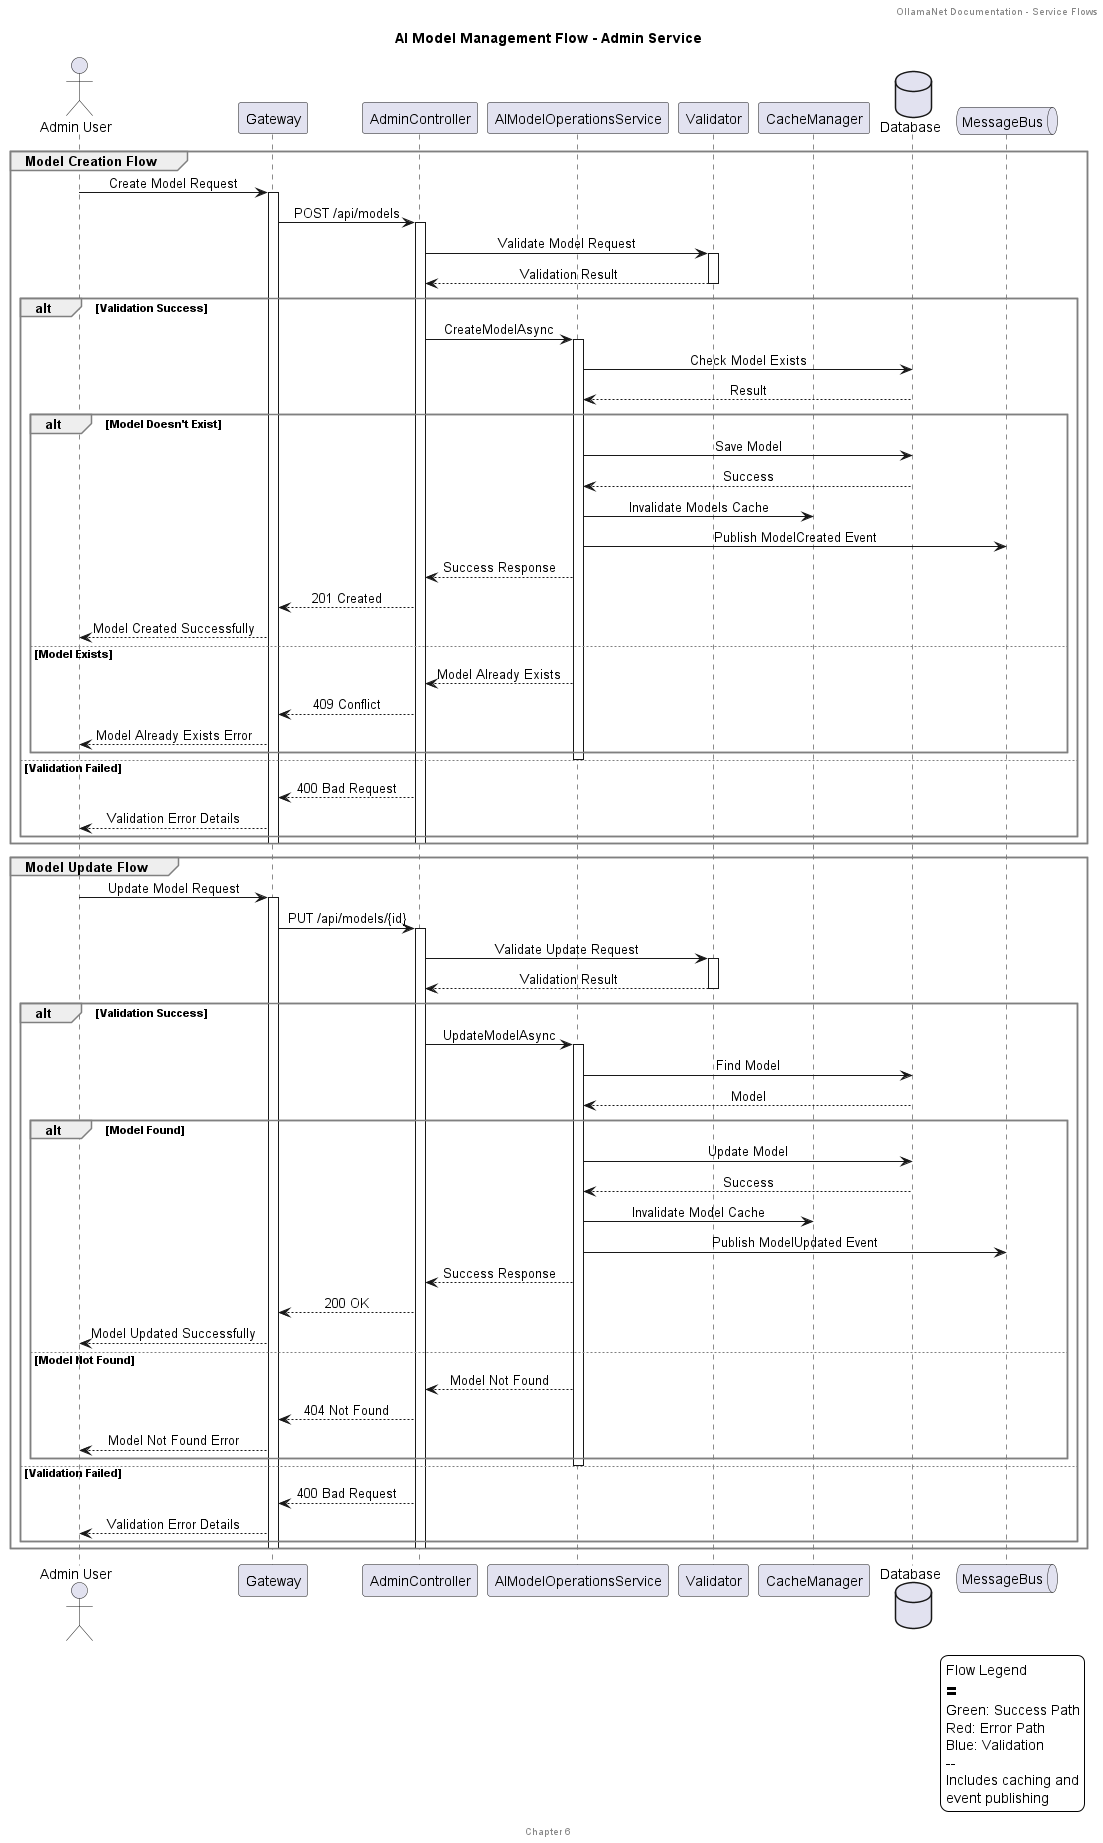
\includegraphics[width=\textwidth]{\chapdir/figures/adminservice_model_management_flow.pdf}
    \caption{AdminService – LLM management flow}
    \label{fig:adminservice-model-flow}
\end{sidewaysfigure}

\subsection{Service-specific Components}
\begin{itemize}
  \item \emph{CacheManager} + Redis two-tier cache.
  \item Ollama integration client for on-demand model installation.
  \item Message handlers for RabbitMQ service-discovery events.
\end{itemize}

\subsection{Integration Points}
AdminService interacts with:
\begin{itemize}
  \item AuthService (JWT validation);
  \item InferenceService (model install / delete APIs);
  \item RabbitMQ (broadcast inference URL changes).
\end{itemize}

% =============================================================
\section{AuthService}
\subsection{Purpose \& Responsibility}
AuthService secures the platform by handling authentication and authorisation.  It issues short-lived JWTs and manages refresh tokens via secure HTTP-only cookies.

\subsection{API Design}
\begin{itemize}
  \item \textbf{POST} \texttt{/api/Auth/Login} – user login (JWT + refresh cookie);
  \item \textbf{POST} \texttt{/api/Auth/Refresh} – obtain new JWT;
  \item \textbf{POST} \texttt{/api/Auth/Register} – create account.
\end{itemize}

\subsection{Data Model}
\begin{itemize}
  \item Identity entities: \textbf{ApplicationUser}, \textbf{Role}, \textbf{RefreshToken}.
\end{itemize}

\subsection{Sequence Diagrams}
\begin{sidewaysfigure}[h]
    \centering
    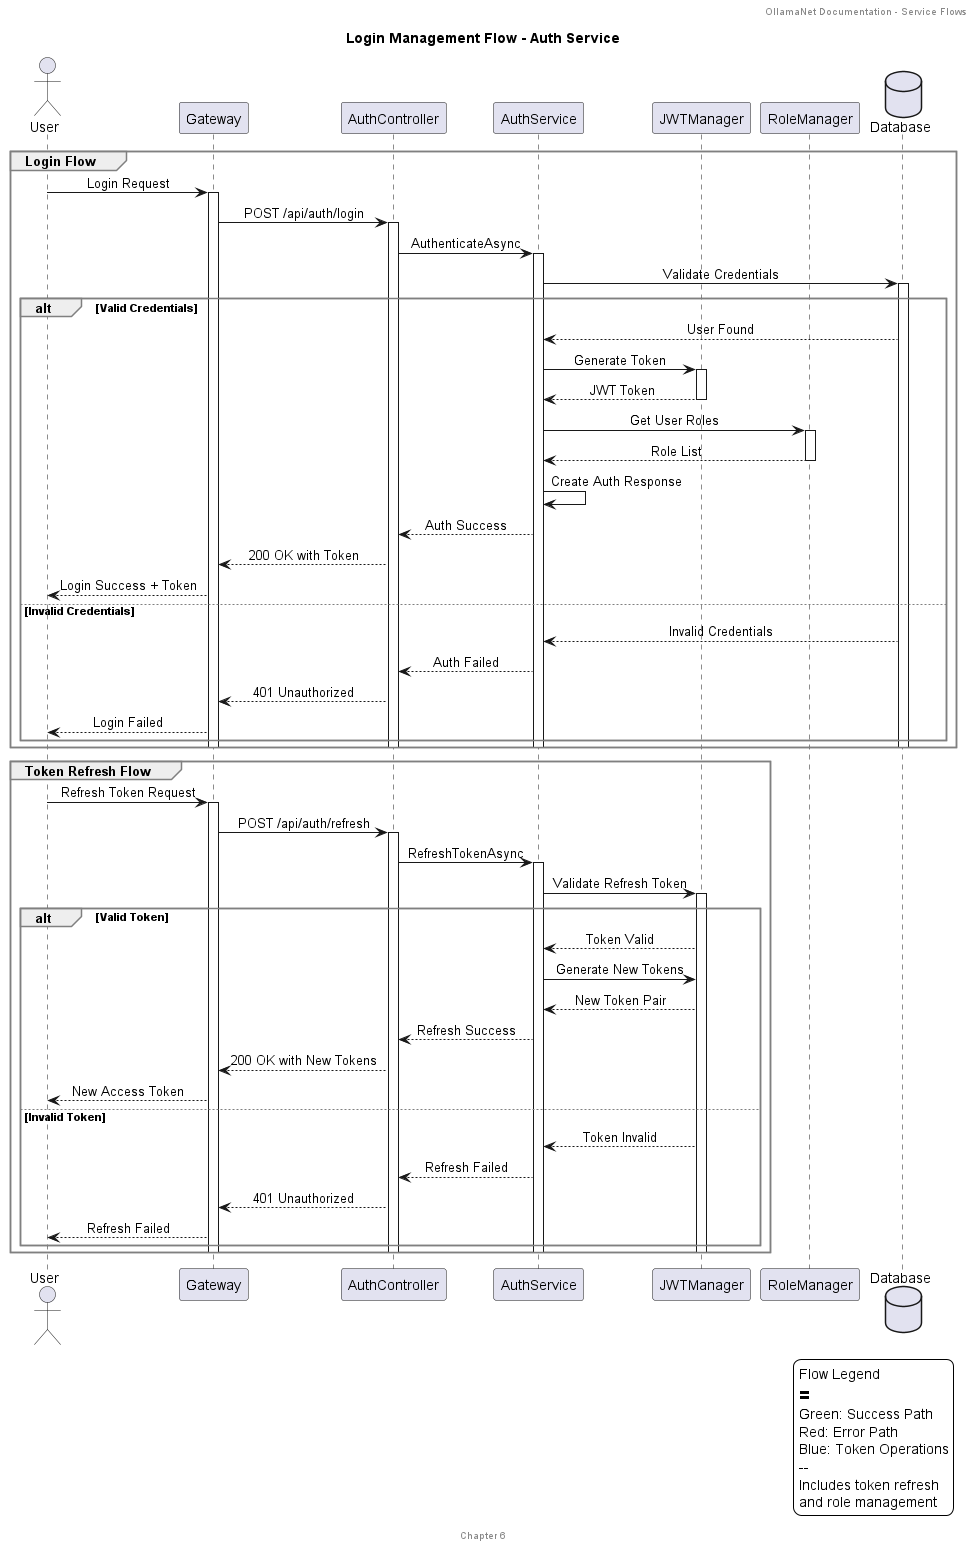
\includegraphics[width=\textwidth]{\chapdir/figures/authservice_login_flow.pdf}
    \caption{AuthService – Login flow}
\end{sidewaysfigure}

\subsection{Service-specific Components}
\begin{itemize}
  \item Password hashing with ASP.NET Core Identity;
  \item Refresh-token rotation with revocation list;
  \item Email sender for verification / reset.
\end{itemize}

\subsection{Integration Points}
Consumes AdminService role data; issues JWTs to every other service.

% =============================================================
\section{ExploreService}
\subsection{Purpose \& Responsibility}
Allows users to discover, filter and search available LLMs.

\subsection{API Design}
\begin{itemize}
  \item \textbf{GET} \texttt{/api/Explore/Models} – list models (pagination, filter by tag);
  \item \textbf{GET} \texttt{/api/Explore/Models/\{id\}} – detailed model info.
\end{itemize}

\subsection{Data Model}
\begin{itemize}
  \item \textbf{LLM}, \textbf{Tag}, \textbf{ModelTag} relationships.
\end{itemize}

\subsection{Sequence Diagrams}
\begin{sidewaysfigure}[h]
    \centering
    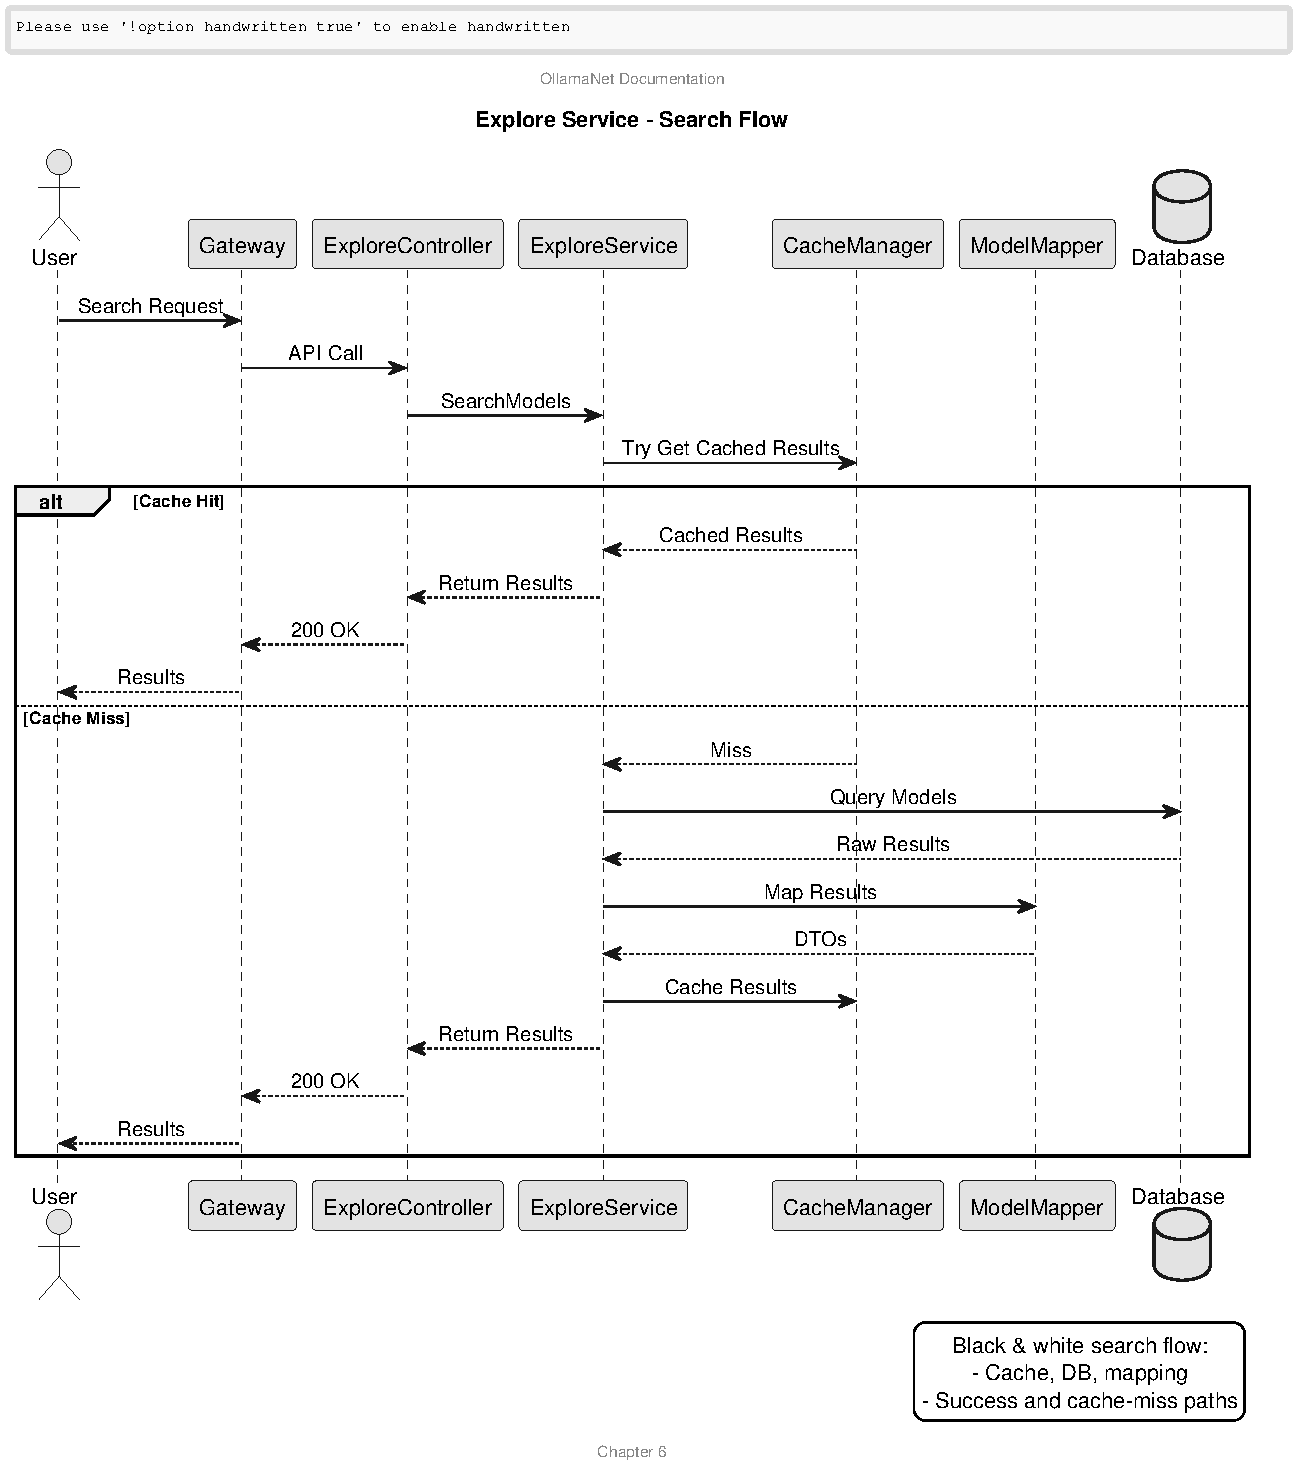
\includegraphics[width=\textwidth]{\chapdir/figures/exploreservice_search_flow.pdf}
    \caption{ExploreService – Tag search flow}
\end{sidewaysfigure}

\subsection{Service-specific Components}
\begin{itemize}
  \item Redis-backed read-through caching;
  \item Domain exceptions hierarchy for robust error reporting.
\end{itemize}

\subsection{Integration Points}
Reads model catalog maintained by AdminService; exposed to UI / external clients.

% =============================================================
\section{ConversationService}
\subsection{Purpose \& Responsibility}
Manages chat threads, message storage, and conversation context for LLM sessions.

\subsection{API Design}
\begin{itemize}
  \item \textbf{GET} \texttt{/api/Conversation/Conversations} – list conversations;
  \item \textbf{POST} \texttt{/api/Conversation/Conversations} – create conversation.
\end{itemize}

\subsection{Data Model}
Entities: \textbf{Conversation}, \textbf{Message}, \textbf{Attachment}, \textbf{LLMResponse}.

\subsection{Sequence Diagrams}
% Placeholder figure commented out.

\subsection{Service-specific Components}
\begin{itemize}
  \item Repository layer with soft-delete for messages;
  \item Saga-style workflow coordinating message save and inference call.
\end{itemize}

\subsection{Integration Points}
Calls InferenceService for streaming completions; publishes events to NotificationService (future work).

% =============================================================
\section{InferenceService}
\subsection{Purpose \& Responsibility}
Hosts the local Ollama engine and exposes HTTP endpoints (proxied by ngrok) for text generation.

\subsection{API Design}
\begin{itemize}
  \item \textbf{POST} \texttt{/api/chat} – single request/response completion;
  \item \textbf{POST} \texttt{/api/chat?stream=true} – streaming completion.
\end{itemize}

\subsection{Service-specific Components}
\begin{itemize}
  \item Notebook-based process manager that boots Ollama and ngrok;
  \item RabbitMQ publisher announcing public URL updates.
\end{itemize}

\subsection{Integration Points}
Consumed by ConversationService and AdminService.

% =============================================================
\section*{Glossary}
\begin{description}
  \item[AdminService] Platform administration micro-service.
  \item[AuthService] Authentication / authorisation micro-service.
  \item[ExploreService] Model discovery micro-service.
  \item[ConversationService] Chat and message management micro-service.
  \item[InferenceService] Ollama-powered text generation micro-service.
  \item[LLM] Large Language Model.
  \item[RabbitMQ] Message broker used for service-discovery events.
\end{description}

\cleardoublepage

\bibliographystyle{\tReferenceStyle}
\bibliography{BibTeX/library,BibTeX/comprehensive}
\appendix
% This is to set the directory this chapter resides in for images
\def\chapdir{./Appendix}

% Title of this chapter
\chapter{An Example Appendix}\label{ap:something}

As an appendix, this should contain some content that's not really required for the argument in the main body of the thesis, but is clearly relevant and supports the work.

\section{Code Listings}\label{sec:code}

The \texttt{listings} package allows you to include code listings or other formatted text with some parsing to make them more readable than simply calling \texttt{\textbackslash{}input\{\}} on the code file.

\definecolor{listinggray}{gray}{0.97}
\lstset{language=python}
\lstset{basicstyle=\scriptsize}
%\lstset{backgroundcolor=listinggray,framerulecolor=blue}
%\lstset{backgroundcolor=listinggray,rulecolor=blue}
\lstset{backgroundcolor=\color{listinggray},rulecolor=\color{blue}}
\lstset{linewidth=\textwidth}
%\lstset{labelstep=10}
%\lstset{commentstyle=\textit, stringstyle=\upshape,stringspaces=false}
%\lstset{commentstyle=\textit, stringstyle=\upshape,showspaces=false}
\lstset{commentstyle=\textit}
\lstset{frame=trbl,frameround=tttt}
\lstinputlisting[caption=\textsc{Matlab} script for interactive radians to degrees converter,label=lst:jacobians]{\chapdir/code.py}

A number of languages are supported with basic syntax highlighting and formatting.



%!TEX root = ../Thesis.tex

\section{Multi-Page Tables}\label{sec:multipagetables}

The \texttt{supertabular} package allows tables to span multiple pages using
the \texttt{supertabular} environment (in place of \texttt{tabular}). This has
already been used in the \hyperref[fr:notation]{Nomenclature Section} in the
front matter, allowing the notation to span multiple pages if necessary.
\autoref{tab:supertabex} shows an example of a table spanning two pages. Note
that such tables are no longer floating elements (i.e.~there's no
\texttt{table} environment anymore), and the header/footer for the whole
table, and ones repeated on each new page, can be defined through
\texttt{supertabular} macros rather than as part of the table to copy headers
across each page.

% Note that it's not in a table environment, since this is NOT a floating environment
\begin{center}
    % Use the supertabular commands rather than the usual caption/etc commands, since they are
    % inserted by supertabular
    \tablecaption[Page-Spanning `Super Table']{This table is especially long, so it's been turned
        into a \texttt{supertabular} environment allowing it to span multiple pages.
        \label{tab:supertabex}}
    % headers and footers can be defined to repeat on each page
    % firsthead and lasttail will be used INSTEAD OF the basic head/tails where appropriate
    \tablefirsthead{%
        \toprule
        \textbf{first} & \textbf{second} & \textbf{RHS}\\
        \midrule[1pt]
    }
    \tablehead{%
        \multicolumn{3}{l}{\small\sl continued from previous page}\\
        \toprule
        \textbf{first} & \textbf{second} & \textbf{RHS}\\
        \midrule
    }
    \tablelasttail{%
        \bottomrule
    }
    \tabletail{%
        \bottomrule
        \multicolumn{3}{l}{\small\sl continued on next page}\\
    }
    % Note that this is JUST the data in the table, since supertabular constructs multiple tables
    % using the firsthead/head/lasttail/tail definitions
    \begin{supertabular}{c @{$\times$} c @{$=$} c}
        1 & 1 & 1 \\
        1 & 2 & 2 \\
        1 & 3 & 3 \\
        1 & 4 & 4 \\
        1 & 5 & 5 \\
        1 & 6 & 6 \\
        1 & 7 & 7 \\
        1 & 8 & 8 \\
        \midrule
        2 & 1 & 2 \\
        2 & 2 & 4 \\
        2 & 3 & 6 \\
        2 & 4 & 8 \\
        2 & 5 & 10\\
        2 & 6 & 12\\
        2 & 7 & 14\\
        2 & 8 & 16\\
        \midrule
        3 & 1 & 3\\
        3 & 2 & 6\\
        3 & 3 & 9\\
        3 & 4 & 12\\
        3 & 5 & 15\\
        3 & 6 & 18\\
        3 & 7 & 21\\
        3 & 8 & 24\\
    \end{supertabular}
\end{center}

\section{Landscape Tables}\label{sec:landscapetables}

If your table is especially wide, it may be better to switch it to the landscape orientation. One way of doing this is with the \texttt{rotating} package, which implements (among other things) two new environments: \texttt{sidewaystable} and \texttt{sidewaysfigure}\footnote{I find \texttt{sidewaysfigure} less useful, as it tends to be easy enough to rotate the figure before inclusion, but if the caption/figure are complex it may be useful to have them oriented in the same way}. The way this package achieves this is most useful for \emph{printed results}, as it only rotates the environment on the page (but does not convert the page into landscape orientation)---for electronic viewing of a PDF, it may be useful to rotate the whole page since it's not often easy for the reader to rotate their screen (assuming the sideways content takes up the whole page). One advantage of this package's implementation of sideways environments is that it supports \texttt{twoside} page layout, and will rotate the sideways environment such that the bottom is towards the outside of the double-page layout in such cases.

An example of a \texttt{sidewaystable} is shown in \autoref{tab:sidewaystable}---if you're reading this as a PDF on your computer, you'll probably find it difficult to read as it's sideways on your
screen.

\begin{sidewaystable}
  \begin{center}
    \caption[Table in Landscape Orientation]{This table is so wide that I decided it should be in
        the landscape orientation to allow it to fit nicely on one page. You may of course find it
        easier (for the reader) to reconsider the content and layout of the table, or convert it to
        a graphical representation, as large walls of data tend to be hard to really interpret well.
        Almost certainly, you'd only have such large tables in an appendix.}
    \label{tab:sidewaystable}
    {\tiny
        % tiny font size because even sideways it wouldn't all fit at the normal font size
        % Note that the {\tiny ...} wraps the whole tabular environment.
    % This table is the output of a matlab script, which I found much easier than handwriting it all.
    \hspace{-14mm}  % HACK to move the table down on the page.
    \begin{tabular}{l c@{\hspace{4pt}}c @{\hspace{4pt}}c @{\hspace{4pt}}c @{\hspace{4pt}}c @{\hspace{4pt}}c @{\hspace{4pt}}c @{\hspace{4pt}}c @{\hspace{4pt}}c @{\hspace{4pt}}c @{\hspace{4pt}}c @{\hspace{4pt}}c @{\hspace{4pt}}c @{\hspace{4pt}}c @{\hspace{4pt}}c @{\hspace{4pt}}c @{\hspace{4pt}}c @{\hspace{4pt}}c @{\hspace{4pt}}c@{}}
      \toprule
      Item & Total &  1 &  2 &  3 &  4 &  5 &  6 &  7 &  8 &  9 & 10 & 11 & 12 & 13 & 14 & 15 & 16 & 17 & 18 \\
      \midrule
      SA Mission Distance (m) & 1101.4 & 49.4 & 81.5 & 34.2 & 78.8 & 98.8 & 70.8 & 16.0 & 61.4 & 14.9 & 52.1 & 24.3 & 83.3 & 170.3 & 143.5 & 20.7 & 30.1 & 21.4 & 99.2 \\
      SA Traversed Distance  (m) & 3244.1 & 53.9 & 86.8 & 90.7 & 92.1 & 120.8 & 74.3 & 46.4 & 63.8 & 15.6 & 55.3 & 27.4 & 127.2 & 222.4 & 987.1 & 273.0 & 167.0 & 235.4 & 505.0 \\
      MA Mission Distance (m) & 1083.9 & 59.1 & 81.5 & 34.2 & 78.8 & 98.8 & 70.8 & 16.0 & 61.4 & 14.9 & 52.1 & 24.3 & 83.3 & 170.3 & 143.5 & 20.7 & 30.1 & 21.4 & 81.8 \\
      MA Traversed Distance  (m) & 2343.1 & 61.8 & 84.6 & 70.7 & 84.6 & 116.6 & 72.5 & 46.3 & 62.6 & 15.5 & 53.5 & 25.8 & 129.4 & 213.4 & 147.1 & 268.2 & 174.5 & 233.8 & 482.3 \\
      \cmidrule(lr){2-20}
      Ratio (SA/MA) & 1.38 & 0.872 & 1.03 & 1.28 & 1.09 & 1.04 & 1.03 & 1 & 1.02 & 1.01 & 1.03 & 1.06 & 0.983 & 1.04 & 6.71 & 1.02 & 0.957 & 1.01 & 1.05 \\
      \midrule
      SA Mission Est. Time (s) & 734.3 & 32.9 & 54.4 & 22.8 & 52.5 & 65.9 & 47.2 & 10.7 & 40.9 & 9.9 & 34.8 & 16.2 & 55.5 & 113.5 & 95.7 & 13.8 & 20.1 & 14.3 & 66.2 \\
      SA Traversal Time  (s) & 2436.0 & 43.5 & 61.6 & 70.1 & 68.0 & 89.6 & 55.3 & 35.2 & 45.3 & 12.7 & 39.8 & 21.8 & 93.1 & 161.8 & 731.0 & 204.7 & 146.1 & 174.3 & 382.1 \\
      MA Mission Est. Time (s) & 1083.9 & 59.1 & 81.5 & 34.2 & 78.8 & 98.8 & 70.8 & 16.0 & 61.4 & 14.9 & 52.1 & 24.3 & 83.3 & 170.3 & 143.5 & 20.7 & 30.1 & 21.4 & 81.8 \\
      MA Traversal Time  (s) & 2411.3 & 64.2 & 84.8 & 73.6 & 86.8 & 119.1 & 74.2 & 47.2 & 63.5 & 16.1 & 54.3 & 28.1 & 132.8 & 215.2 & 148.2 & 271.3 & 203.4 & 239.9 & 488.7 \\
      \cmidrule(lr){2-20}
      Ratio (SA/MA) & 1.01 & 0.677 & 0.726 & 0.953 & 0.784 & 0.753 & 0.746 & 0.744 & 0.714 & 0.786 & 0.734 & 0.776 & 0.701 & 0.752 & 4.93 & 0.755 & 0.718 & 0.727 & 0.782 \\
      \midrule
      SA Cost (Exp.~Map)  & 1019924.1 & 1540.6 & 49041.0 & 5094.7 & 86202.5 & 98847.3 & 0.0 & 7974.8 & 1773.9 & 459.0 & 7825.8 & 1120.0 & 4131.3 & 14618.2 & 447306.7 & 19380.5 & 109612.1 & 33188.1 & 131807.7 \\
      MA Cost (Exp.~Map)  & 916661.5 & 6032.4 & 81939.1 & 7722.2 & 73856.9 & 198949.4 & 11654.8 & 6191.5 & 1398.9 & 564.8 & 13336.9 & 1123.8 & 6129.8 & 68857.2 & 39422.7 & 3213.2 & 172319.0 & 93562.5 & 130386.5 \\
      \cmidrule(lr){2-20}
      Ratio (SA/MA) & 1.11 & 0.255 & 0.599 & 0.66 & 1.17 & 0.497 & 0 & 1.29 & 1.27 & 0.813 & 0.587 & 0.997 & 0.674 & 0.212 & 11.3 & 6.03 & 0.636 & 0.355 & 1.01 \\
      \midrule
      SA Cost (Ground Truth)  & 26891.4 & 0.0 & 0.0 & 0.0 & 0.0 & 0.0 & 0.0 & 0.0 & 0.0 & 0.0 & 0.0 & 0.0 & 0.0 & 0.0 & 0.0 & 0.0 & 26891.4 & 0.0 & 0.0 \\
      MA Cost (Ground Truth)  & 28400.0 & 0.0 & 0.0 & 0.0 & 0.0 & 0.0 & 0.0 & 0.0 & 0.0 & 0.0 & 0.0 & 0.0 & 0.0 & 0.0 & 0.0 & 0.0 & 28400.0 & 0.0 & 0.0 \\
      \cmidrule(lr){2-20}
      Ratio (SA/MA) & 0.947 & -- & -- & -- & -- & -- & -- & -- & -- & -- & -- & -- & -- & -- & -- & -- & 0.947 & -- & -- \\
      \bottomrule
    \end{tabular}
    \begin{tabular}{l c c c}
    \noalign{\vspace{2ex}}
      \toprule
      Map Configuration & SA Coverage ($\textrm{m}^2$) & MA Coverage ($\textrm{m}^2$) & Ratio (MA/SA) \\
      \midrule
      Expanded Cost Map &   28108 &   28229 &     1 \\
      \bottomrule
    \end{tabular}
    }
  \end{center}
\end{sidewaystable}





\end{document}
